\documentclass[11pt]{article}

\usepackage[a4paper,margin=1in]{geometry}
\usepackage{amsmath,amssymb,bm}
\usepackage{graphicx}
\usepackage[hypertexnames=false]{hyperref}
\usepackage{booktabs}
\usepackage{float}
\usepackage[section]{placeins}
\usepackage{array}
\usepackage{caption}
\usepackage{subcaption}
\usepackage{xcolor}

\newcommand{\q}{\mathbf q}
\newcommand{\qp}{\mathbf q_p}
\newcommand{\qs}{\mathbf q_s}
\newcommand{\qbar}{\overline{\mathbf q}}
\newcommand{\V}{\mathbf V}
\newcommand{\uvec}{\mathbf u}
\newcommand{\mub}{\bm\mu}
\newcommand{\R}{\mathbf R}
\newcommand{\J}{\mathbf J}
\newcommand{\z}{\mathbf z}
\newcommand{\norm}[1]{\left\lVert #1 \right\rVert}

% Title option 1:
% Nonlinear latent manifolds and closure models for reduced order models
% Title option 2:
% Learned Closures and Nonlinear Latent Manifolds for ANN-Enhanced Reduced-Order Models
\title{\vspace{-1.5em}
Learned closures and nonlinear manifolds for parametric projection-based reduced models}
\author{S. Ares de Parga, Y. Maday}
\date{\today}

\begin{document}
\maketitle
\vspace{-1.0em}

\begin{abstract}
This work presents a comparative assessment of learned closures and nonlinear
manifolds for parametric projection-based reduced-order models of nonlinear
time-dependent systems. Within a common reduced-coordinate representation, we
compare state-conditioned, parameter--time-conditioned, and hybrid neural
closures; an intrusive autoencoder decoder manifold; a non-intrusive direct
coefficient map; and a non-intrusive latent POD-DL-ROM. The framework is
evaluated on a parametric two-dimensional inviscid Burgers benchmark using both
full-residual projection and empirical-cubature hyperreduction.

The study separates three sources of error: the reduced trial representation,
the learned-coordinate approximation, and residual hyperreduction. A
metric-aware trial basis is designed to limit the transfer of unresolved
coordinate errors into residual-solved coordinates. ROM-consistent linear
projection trajectories provide the learning targets, which permits data
enrichment without acquiring additional high-dimensional snapshots. Controlled
dimension and tail-perturbation diagnostics show that a parameter--time
closure can feed its secondary-coordinate error back into an intrusive LSPG
solve. Enlarging the coefficient training set substantially reduces this
effect and improves the intrusive and non-intrusive learned models. The
results clarify which error mechanisms are due to the learned manifold and
which are introduced by hyperreduction, providing a reproducible basis for
selecting closure architectures and training data in projection-based ROMs.
\end{abstract}

\vspace{-1.0em}

\section{Introduction}
Projection-based model order reduction (PMOR) is a standard framework for reducing high-dimensional parametric models while preserving governing equations \cite{antoulas2005approximation,quarteroni2014reduced}. For nonlinear transport-dominated dynamics, linear subspaces may require large dimensions, which motivates nonlinear manifolds, closure modeling, and latent representations \cite{barnett2023neural,cohen2023nonlinear,aghili2026nonlinear}.

From a machine-learning viewpoint, four families are relevant to this work:
\begin{itemize}
\item intrusive closure-enhanced projection (PROM-ANN) \cite{barnett2023neural},
\item intrusive latent-manifold projection (PROM-POD-AE), in the spirit of hyperreduced nonlinear manifold ROMs \cite{romor2025explicable},
\item non-intrusive direct-coefficient regression maps $(\bm\mu,t)\mapsto\mathbf q_N$,
\item non-intrusive latent POD-DL-ROM maps \cite{fresca2022pod}.
\end{itemize}

\paragraph{Naming convention used in this manuscript.}
When we say \textbf{POD-NN-ROM}, we refer to the non-intrusive coefficient-space
map $(\bm\mu,t)\mapsto\mathbf q_N$. When we say \textbf{POD-DL-ROM}, we refer to
the non-intrusive latent family in the sense of Fresca--Manzoni
\cite{fresca2022pod}. When we say \textbf{PROM-POD-AE}, we refer
to an intrusive latent-manifold projection route (conceptually aligned with
intrusive nonlinear-manifold HPROM literature such as \cite{romor2025explicable}),
even though those references use different method names.

The goal is a controlled comparison under strong online compression.  All variants use the same HDM residual, time discretization, and fixed trial basis.  The PROM experiments evaluate the full residual, whereas the HPROM experiments use model-matched empirical-cubature-method (ECM) rules; this separation exposes the effect of residual sampling instead of conflating it with regression error.

\section{Linear PROM/HPROM Reference and Notation}
\label{sec:linear-rom}

\subsection{Generic semi-discrete IVP and residual notation}
Given the generic, parametric, nonlinear, semi-discrete, first-order initial
value problem
\begin{equation}
\mathbf M(\bm\mu)\,\dot{\mathbf u}(t;\bm\mu)
\;+\;
\mathbf f\!\left(\mathbf u(t;\bm\mu);\bm\mu\right)
\;-\;
\mathbf g(t;\bm\mu)
\;=\;\mathbf 0,
\qquad
\mathbf u(0;\bm\mu)=\mathbf u_0(\bm\mu),
\label{eq:generic-ivp}
\end{equation}
with $\bm\mu\in\mathcal D\subset\mathbb R^p$, we denote by
$\mathbf r^{m+1}$ the nonlinear time-discrete residual associated with the
selected implicit time integrator. In compact form, each HDM step is written
as
\begin{equation}
\mathbf r^{m+1}\!\left(\mathbf u^{m+1};\bm\mu\right)=\mathbf 0.
\label{eq:generic-discrete-residual}
\end{equation}
For readability, dependencies on previous time states and $\Delta t$ are kept
implicit in $\mathbf r^{m+1}$.

\subsection{POD basis from SVD}
Let $\mathbf u(t;\bm\mu)\in\mathbb R^N$ denote the HDM state with parameters $\bm\mu\in\mathcal D\subset\mathbb R^p$. Define
\begin{equation}
\mathbf u_{\mathrm{ref}}:=\frac{1}{N_s}\sum_{i=1}^{N_s}\mathbf u^i,
\qquad
\mathbf S_c=[\mathbf u^1-\mathbf u_{\mathrm{ref}}\ \cdots\ \mathbf u^{N_s}-\mathbf u_{\mathrm{ref}}].
\end{equation}
Let
\begin{equation}
\mathbf S_c=\mathbf U_{\mathbf S}\mathbf\Sigma_{\mathbf S}\mathbf Y_{\mathbf S}^T
\end{equation}
be its thin SVD, and define the linear ROB
\begin{equation}
\mathbf V_{\mathrm{tot}}\in\mathbb R^{N\times n_{\mathrm{tot}}}
\end{equation}
as the first $n_{\mathrm{tot}}$ left singular vectors of $\mathbf U_{\mathbf S}$.

The linear reduced reconstruction is
\begin{equation}
\tilde{\mathbf u}(t;\bm\mu)=\mathbf u_{\mathrm{ref}}+\mathbf V_{\mathrm{tot}}\mathbf q_N(t;\bm\mu),
\qquad
\mathbf q_N(t;\bm\mu)\in\mathbb R^{n_{\mathrm{tot}}}.
\label{eq:linear-reconstruction}
\end{equation}

\subsection{Linear time-discrete LSPG reference form}
Let $\mathbf r^{m+1}(\mathbf u;\bm\mu)\in\mathbb R^N$ denote the HDM time-discrete residual at step $m{+}1$. The unsampled reference linear LSPG solve is
\begin{equation}
\mathbf q_N^{m+1}(\bm\mu)
=
\arg\min_{\mathbf x\in\mathbb R^{n_{\mathrm{tot}}}}
\left\|
\mathbf r^{m+1}\!\left(\mathbf u_{\mathrm{ref}}+\mathbf V_{\mathrm{tot}}\mathbf x;\bm\mu\right)
\right\|_2^2.
\label{eq:linear-lspg-min}
\end{equation}

With
\begin{equation}
\mathbf J^{m+1,k}:=\frac{\partial\mathbf r^{m+1}}{\partial\mathbf u},
\qquad
\mathbf T_N:=\mathbf V_{\mathrm{tot}},
\qquad
\mathbf W_N^{m+1,k}:=\mathbf J^{m+1,k}\mathbf T_N,
\end{equation}
the Gauss--Newton increment solves
\begin{equation}
(\mathbf W_N^{m+1,k})^T\mathbf W_N^{m+1,k}\,\Delta\mathbf q_N^{m+1,k}
=
-(\mathbf W_N^{m+1,k})^T
\mathbf r^{m+1}\!\left(\mathbf u_{\mathrm{ref}}+\mathbf V_{\mathrm{tot}}\mathbf q_N^{m+1,k};\bm\mu\right).
\label{eq:linear-gn-update}
\end{equation}

\subsection{Linear HPROM via the empirical cubature method}
Let $\mathcal E=\{e_i\}_{i=1}^{N_e}$ denote the set of mesh entities. The
time-discrete residual is assembled from local contributions,
\begin{equation}
\mathbf r^{m+1}(\mathbf u;\bm\mu)
=
\sum_{e_i\in\mathcal E}
\mathbf L_{e_i}^{T}
\mathbf r_{e_i}^{m+1}
\!\left(\mathbf L_{e_i^+}\mathbf u;\bm\mu\right).
\label{eq:elementwise-residual}
\end{equation}
Here $\mathbf r_{e_i}^{m+1}\in\mathbb R^{d_{e_i}}$ is the residual associated
with entity $e_i$, $\mathbf L_{e_i}\in\{0,1\}^{d_{e_i}\times N}$ extracts its
residual degrees of freedom, and $\mathbf L_{e_i^+}$ extracts the enlarged
stencil needed to evaluate that contribution.  The latter includes neighboring
entities whenever the spatial discretization requires them.

For the affine trial manifold
$\boldsymbol\phi_N(\mathbf q_N)=\mathbf u_{\mathrm{ref}}+\mathbf V_{\mathrm{tot}}\mathbf q_N$,
consider Gauss--Newton iteration $k$ at time step $m+1$.  With
\begin{equation}
\mathbf T_N=\mathbf V_{\mathrm{tot}},
\qquad
\mathbf J^{m+1,k}=\frac{\partial\mathbf r^{m+1}}{\partial\mathbf u}
\bigg|_{\boldsymbol\phi_N(\mathbf q_N^{m+1,k})},
\qquad
\mathbf W_N^{m+1,k}=\mathbf J^{m+1,k}\mathbf T_N,
\label{eq:linear-hprom-test-basis}
\end{equation}
the projected LSPG residual has the entity-wise representation
\begin{equation}
\begin{aligned}
\mathbf r_N^{m+1,k}(\bm\mu)
&:=(\mathbf W_N^{m+1,k})^{T}\mathbf r^{m+1}
\!\left(\boldsymbol\phi_N(\mathbf q_N^{m+1,k});\bm\mu\right) \\
&=
\sum_{e_i\in\mathcal E}
\left(\mathbf L_{e_i}\mathbf W_N^{m+1,k}\right)^T
\mathbf r_{e_i}^{m+1}
\!\left(\mathbf L_{e_i^+}\boldsymbol\phi_N(\mathbf q_N^{m+1,k});\bm\mu\right).
\end{aligned}
\label{eq:linear-projected-residual}
\end{equation}
Let
$\mathbf J_{e_i}^{m+1,k}=\partial\mathbf r_{e_i}^{m+1}/\partial(\mathbf L_{e_i^+}\mathbf u)$
at the same state. The Gauss--Newton matrix is assembled analogously,
\begin{equation}
\mathbf J_N^{m+1,k}
:=
(\mathbf W_N^{m+1,k})^T\mathbf J^{m+1,k}\mathbf T_N
=
\sum_{e_i\in\mathcal E}
\left(\mathbf L_{e_i}\mathbf W_N^{m+1,k}\right)^T
\mathbf J_{e_i}^{m+1,k}
\left(\mathbf L_{e_i^+}\mathbf T_N\right).
\label{eq:linear-projected-jacobian}
\end{equation}
ECM selects a reduced mesh $\widetilde{\mathcal E}_N\subset\mathcal E$ and
positive weights $\xi_{N,e_i}$ that approximate both sums with the same
cubature rule:
\begin{equation}
\begin{aligned}
\widehat{\mathbf r}_N^{m+1,k}
&=
\sum_{e_i\in\widetilde{\mathcal E}_N}\xi_{N,e_i}
\left(\mathbf L_{e_i}\mathbf W_N^{m+1,k}\right)^T
\mathbf r_{e_i}^{m+1}
\!\left(\mathbf L_{e_i^+}\boldsymbol\phi_N(\mathbf q_N^{m+1,k});\bm\mu\right),\\
\widehat{\mathbf J}_N^{m+1,k}
&=
\sum_{e_i\in\widetilde{\mathcal E}_N}\xi_{N,e_i}
\left(\mathbf L_{e_i}\mathbf W_N^{m+1,k}\right)^T
\mathbf J_{e_i}^{m+1,k}
\left(\mathbf L_{e_i^+}\mathbf T_N\right).
\end{aligned}
\label{eq:linear-ecm-sampled-normal-equations}
\end{equation}
The sampled Gauss--Newton update is therefore
\begin{equation}
\widehat{\mathbf J}_N^{m+1,k}\Delta\mathbf q_N^{m+1,k}
=-\widehat{\mathbf r}_N^{m+1,k},
\qquad
\mathbf q_N^{m+1,k+1}
=\mathbf q_N^{m+1,k}+\Delta\mathbf q_N^{m+1,k}.
\label{eq:linear-hprom-gn-update}
\end{equation}

\paragraph{Offline cubature construction.}
At each selected parameter--time state $s$, the linear reduced coordinate
$\mathbf q_{N,s}$ and the associated test basis $\mathbf W_{N,s}$ define the
contribution of entity $e_i$ as
\begin{equation}
\mathbf c_{N,e_i}^{(s)}
=
\left(\mathbf L_{e_i}\mathbf W_{N,s}\right)^T
\mathbf r_{e_i}
\!\left(\mathbf L_{e_i^+}\boldsymbol\phi_N(\mathbf q_{N,s});\bm\mu_s\right).
\label{eq:linear-ecm-training-contribution}
\end{equation}
Stacking these $n_{\mathrm{tot}}$-vectors over the $N_{\mathrm{ECM}}$
selected states gives
\begin{equation}
\mathbf C_N=
\begin{bmatrix}
\mathbf c_{N,e_1}^{(1)} & \cdots & \mathbf c_{N,e_{N_e}}^{(1)}\\
\vdots & & \vdots\\
\mathbf c_{N,e_1}^{(N_{\mathrm{ECM}})} & \cdots &
\mathbf c_{N,e_{N_e}}^{(N_{\mathrm{ECM}})}
\end{bmatrix}
\in\mathbb R^{n_{\mathrm{tot}}N_{\mathrm{ECM}}\times N_e},
\qquad
\mathbf b_N=\mathbf C_N\mathbf 1.
\label{eq:linear-ecm-training-matrix}
\end{equation}
The empirical cubature method computes a sparse nonnegative approximation of
the full projected residual data,
\begin{equation}
\boldsymbol\xi_N
=
\arg\min_{\boldsymbol\zeta\geq\mathbf0}
\left\|\mathbf C_N\boldsymbol\zeta-\mathbf b_N\right\|_2^2,
\qquad
\widetilde{\mathcal E}_N
=\left\{e_i\in\mathcal E:\xi_{N,e_i}>0\right\}.
\label{eq:linear-ecm-cubature}
\end{equation}
In the present implementation, a direct SVD is used to remove numerically
null directions of $\mathbf C_N$ before the nonnegative cubature solve. The
rule is therefore tied to the reduced manifold and its LSPG test basis.
Consequently, the linear rule cannot be reused after replacing the affine
trial space by a learned closure or decoder manifold
\cite{hernandez2017dimensional,hernandez2020multiscale,de2023hyper,ares2026closure}.

\paragraph{Shared hyper-reduction principle.}
The common algebraic step is to assemble entity-wise contributions to the
projected LSPG residual and approximate their sum with a sparse positive
rule.  Several hyperreduction strategies fit this project--then--approximate
view.  Energy-conserving sampling and weighting (ECSW), for example, acts on
the same type of projected contributions \cite{farhat2015structure}.  We use
ECM throughout this work, following the empirical-cubature construction of
\cite{hernandez2017dimensional,hernandez2020multiscale}; the distinction is
methodological, not a change to the reduced manifold or LSPG formulation.

\paragraph{Reduced-order training targets.}
The PROM campaigns use trajectories $\mathbf q_N(t;\bm\mu)$ generated by the full-residual linear LSPG solve
\eqref{eq:linear-lspg-min}; the HPROM campaigns use the corresponding linear HPROM trajectories generated by
the sampled update \eqref{eq:linear-hprom-gn-update}. This convention applies to every learned family in this work, including the direct
POD--NN-ROM and POD--DL-ROM maps.  Thus, no learned target is obtained by orthogonally projecting HDM snapshots.
The choice is deliberate: each learned map approximates relations between coordinates generated by the same type of
reduced optimality problem used in its online comparison.  It prevents a projection target from being mixed with
LSPG or HPROM dynamics and allows the PROM and HPROM studies to isolate full-residual and residual-sampling
effects, respectively.  A conventional purely non-intrusive workflow would instead train on HDM snapshots projected
onto the trial space; we retain the ROM-generated targets here to make the direct maps, the Case~2 closure, and their
intrusive counterparts directly comparable.

\section{Metric-Aware Basis Construction for Closure Robustness}
\label{sec:metric-aware-basis}

The intrusive closure constructions introduced in Section~\ref{sec:method-ann}
partition the common linear basis as
$\mathbf V_{\mathrm{tot}}=[\mathbf V\ \overline{\mathbf V}]$, with online
coordinates $\mathbf q$ and reconstructed coordinates $\bar{\mathbf q}$.
This partition is not only an approximation choice: in an intrusive LSPG
solve, errors in the reconstructed high-order coordinates can feed back into
the low-order coordinates through the residual normal equations. The same
$\mathbf V_{\mathrm{tot}}$ also defines the coordinate system used by the
decoder and direct regression models. Consequently, the metric used to
construct the basis is part of the common robustness design, rather than a
model-specific preprocessing choice.

\subsection{Euclidean and M-regularized LSPG-sensitive metrics}
For comparison, the Euclidean POD basis is obtained from the centered snapshot
matrix $\mathbf S_c$. We also consider a residual-sensitive metric
that combines a physical mass contribution with an averaged LSPG sensitivity:
\begin{equation}
\mathbf W
=
\varepsilon\,\mathbf M
+
\sum_{s\in\mathcal S_{\mathrm{met}}}
\omega_s\,
(\mathbf J_s)^T\mathbf P_s\mathbf J_s .
\label{eq:mlspg-metric}
\end{equation}
Here $\mathbf M$ is the block mass/area matrix associated with the state
inner product, $\mathbf J_s=\partial\mathbf r_s/\partial\mathbf u$ is the
time-discrete residual Jacobian at a selected snapshot, $\mathbf P_s$ is the
nonnegative sampling/weighting operator used for the residual metric, and
$\omega_s$ are quadrature and parameter weights. The small positive parameter
$\varepsilon$ regularizes the metric and preserves physical state weighting
when the residual sensitivity is weak or locally rank deficient.

The corresponding weighted POD basis is obtained from the generalized
correlation matrix
\begin{equation}
\mathbf C
=
\mathbf S_c^T\mathbf W\mathbf S_c .
\label{eq:mlspg-correlation}
\end{equation}
If $\mathbf C\mathbf y_i=\lambda_i\mathbf y_i$, the associated
modes are
\begin{equation}
\bm\phi_i
=
\frac{1}{\sqrt{\lambda_i}}\mathbf S_c\mathbf y_i,
\qquad
\bm\phi_i^T\mathbf W\bm\phi_j=\delta_{ij}.
\label{eq:weighted-pod-modes}
\end{equation}
In practice, the metric is assembled on a representative subset of parameter
and time samples, selected independently from the final test points. The
resulting basis is then used uniformly by all reduced models; it is not tuned
separately for a particular closure map.

\paragraph{Reported metric configuration.}
For the Burgers basis used throughout this paper, the nine baseline parameter
trajectories provide $4500$ candidate non-initial snapshot columns.  We retain
$2250$ centered snapshot columns and $2250$ metric samples through the same
global parameter--time stratified rule, with uniform parameter weights and
trapezoidal time weights.  We use $\mathbf P_s=\mathbf I$ in
Eq.~\eqref{eq:mlspg-metric}.  The regularization is set by the trace-ratio rule
\begin{equation}
  \varepsilon = \eta\,\frac{\operatorname{tr}(\mathbf C_J)}
  {\operatorname{tr}(\mathbf C_M)},
  \qquad \eta=10^{-10},
  \label{eq:metric-trace-ratio}
\end{equation}
where $\mathbf C_M=\mathbf S_c^T\mathbf M\mathbf S_c$ and $\mathbf C_J$
is the sensitivity contribution to Eq.~\eqref{eq:mlspg-correlation}.  This
gives $\varepsilon=6.2555\times10^{-10}$ for the reported data.  The retained
$n_{\mathrm{tot}}=151$ modes capture $99.9883\%$ of the weighted snapshot
energy.  Thus the small mass contribution regularizes the metric scale without
overriding the LSPG-sensitivity term.

\subsection{Low/high transfer diagnostic}
To quantify the potential effect of prescribing a secondary-coordinate block,
consider a local linearization of the LSPG normal equations around a reference
reduced trajectory. Let
\begin{equation}
\mathbf A_s=(\mathbf J_s)^T\mathbf P_s\mathbf J_s,
\qquad
\mathbf H_s=
\begin{bmatrix}
\mathbf V^T\mathbf A_s\mathbf V
&
\mathbf V^T\mathbf A_s\overline{\mathbf V}
\\
\overline{\mathbf V}^T\mathbf A_s\mathbf V
&
\overline{\mathbf V}^T\mathbf A_s\overline{\mathbf V}
\end{bmatrix}.
\end{equation}
If the high coordinates are perturbed by $\delta\bar{\mathbf q}$ and
$\mathbf H_{LL}$ is nonsingular, the corresponding first-order low-coordinate
response is approximated by
\begin{equation}
\delta\mathbf q
\approx
-
\left(\mathbf H_{LL}\right)^{-1}\mathbf H_{LH}\,\delta\bar{\mathbf q}
=
\mathbf T_{LH}\,\delta\bar{\mathbf q}.
\label{eq:low-high-transfer}
\end{equation}
Thus, $\mathbf T_{LH}$ identifies high-coordinate directions that are most
likely to perturb the resolved LSPG coordinates. The purpose of the
$M$-regularized LSPG-sensitive metric is not to optimize one regression map,
but to construct a basis for which this low/high transfer is less amplifying
without compromising the linear reduced representation. The closure maps that
use this partition are defined formally in Section~\ref{sec:method-ann}.

\subsection{Basis-selection criterion}
\label{sec:metric-selection-criterion}
The metric is selected at the level of the common reduced coordinate system,
before choosing a closure architecture or a non-intrusive regressor. It
therefore changes not only the trial space $\mathbf V_{\mathrm{tot}}$, but
also the reduced-coordinate trajectories used as learning targets. Selecting
the metric by the validation loss of one learned map would consequently
confound basis quality with the capacity and optimization of that particular
map.

We instead impose two basis-level requirements. First, at the retained
dimension $n_{\mathrm{tot}}$, the metric must preserve the state accuracy of
the full-coordinate linear LSPG reference. This prevents a reduction in
low/high transfer from being obtained simply by degrading the linear trial
representation. The ECM rules used subsequently are constructed only after
this basis has been fixed and are matched to the relevant trial manifold.
Second, for a partition
$\mathbf q_N=[\mathbf q;\bar{\mathbf q}]$, it should reduce the amplification
measured by \eqref{eq:low-high-transfer}. This second requirement is relevant
whenever a reduced model supplies part of the coordinate vector rather than
solving all $n_{\mathrm{tot}}$ coordinates through the residual; the specific
models considered here are defined in the following sections.

The direct transfer diagnostic and the complementary oracle perturbation test
are reported in Appendix~\ref{app:basis-selection-diagnostics}. Together,
they show that the $M$-regularized LSPG-sensitive basis reduces the
high-to-low coupling while leaving the linear reference essentially unchanged.
Accordingly, unless stated otherwise, every model below uses this single
coordinate basis; the intrusive variants use it as their trial basis. This
common choice is essential: differences among the subsequent models can then
be attributed to the learned coordinate relation and, for HPROMs, to the
model-matched cubature rule rather than to a model-specific trial space.

\section{Method I: PROM-ANN Closure Models}
\label{sec:method-ann}

\subsection{Manifold definitions}
We follow the neural-network-augmented projection framework of
Barnett, Farhat, and Maday \cite{barnett2023neural}, in which a nonlinear
trial manifold augments a retained linear subspace with a learned closure for
the remaining reduced coordinates. Let the common linear trial basis and its
coordinates be partitioned as
\begin{equation}
\mathbf V_{\mathrm{tot}}=[\mathbf V\ \overline{\mathbf V}],
\qquad
\mathbf q_N=
\begin{bmatrix}
\mathbf q\\
\bar{\mathbf q}
\end{bmatrix},
\qquad
n+\bar n=n_{\mathrm{tot}}.
\label{eq:closure-partition}
\end{equation}
The associated linear reduced state is therefore
\begin{equation}
\mathbf u(t;\bm\mu)
\approx
\mathbf u_{\mathrm{ref}}
+\mathbf V\,\mathbf q(t;\bm\mu)
+\overline{\mathbf V}\,\bar{\mathbf q}(t;\bm\mu).
\label{eq:linear-partitioned-state}
\end{equation}
The first block $\mathbf q\in\mathbb R^n$ contains the coordinates retained
as online unknowns; the secondary block
$\bar{\mathbf q}\in\mathbb R^{\bar n}$ contains the remaining coordinates.

PROM--ANN replaces the secondary block by a learned map
\begin{equation}
\bar{\mathbf q}=
\mathcal F(\mathbf q,\bm\mu,t),
\qquad
\mathcal F:\mathbb R^n\times\mathcal D\times[0,T]
\longrightarrow\mathbb R^{\bar n},
\label{eq:closure-map}
\end{equation}
which defines the parameter--time-dependent nonlinear trial manifold
\begin{equation}
\mathcal M_{\mathcal F}(\bm\mu,t)
=
\left\{
\mathbf u_{\mathrm{ref}}+\mathbf V\,\mathbf q
+\overline{\mathbf V}\,\mathcal F(\mathbf q,\bm\mu,t)
\;:\;\mathbf q\in\mathbb R^n
\right\}.
\label{eq:ann-manifold}
\end{equation}
Thus, the network does not approximate the high-dimensional state directly:
it supplies only the secondary reduced coordinates, while the primary
coordinates are determined by the residual minimization described below.

The three closure choices differ only in the information supplied to
$\mathcal F$:
\begin{align}
\text{Case 1:}&\quad \bar{\mathbf q}=\mathcal N(\mathbf q),\\
\text{Case 2:}&\quad \bar{\mathbf q}=\mathcal M(\bm\mu,t),\\
\text{Case 3:}&\quad \bar{\mathbf q}=\mathcal H(\mathbf q,\bm\mu,t).
\end{align}
Case~1 is a state-conditioned closure: the secondary coordinates are inferred
only from the currently solved primary coordinates. Case~2 is a
parameter--time-conditioned closure: at every time step it injects a
secondary-coordinate vector predicted from $(\bm\mu,t)$, independently of
the current primary iterate. Case~3 combines both sources of information.
Consequently, Case~2 has the simplest online tangent, whereas Cases~1 and~3
can adapt the closure as the primary coordinates change during the nonlinear
solve.

\paragraph{Shared Case~2 and POD--NN master map.}
To avoid comparing two different regressors, Case~2 and POD--NN-ROM use the
same parameter--time master map
\begin{equation}
\mathcal G_q:\; (\bm\mu,t)\longmapsto
\widehat{\mathbf q}_N\in\mathbb R^{n_{\mathrm{tot}}}.
\label{eq:master-q-map}
\end{equation}
For a Case~2 split with $n$ primary coordinates, the closure is not trained as
a separate tail-only network; it is the selected secondary block of this map,
\begin{equation}
\mathcal M_n(\bm\mu,t)
=\mathbf P_{>n}\mathcal G_q(\bm\mu,t),
\qquad
\mathbf P_{>n}\widehat{\mathbf q}_N
=\widehat{\bar{\mathbf q}}\in\mathbb R^{n_{\mathrm{tot}}-n}.
\label{eq:case2-master-tail}
\end{equation}
Case~2 inserts $\mathcal M_n$ into the LSPG solve for the first $n$
coordinates, whereas POD--NN-ROM uses the complete vector
$\mathcal G_q(\bm\mu,t)$ directly.  Therefore $n=0$ is exactly the
POD--NN-ROM prediction from the same trained network, rather than a merely
similar model.

In the $n_{\mathrm{tot}}$-dimensional linear PROM or linear HPROM reference
used for target generation, both $\mathbf q$ and $\bar{\mathbf q}$ are solved
online. In the PROM--ANN models, only $\mathbf q$ remains an online unknown;
the secondary coordinates are evaluated from the learned closure. This is an
$n$-dimensional nonlinear manifold embedded in the same
$n_{\mathrm{tot}}$-dimensional coefficient space used to generate the
training targets.

The three cases differ in how the closure interacts with the LSPG tangent. In
Case~1 and Case~3 the tangent contains
$\overline{\mathbf V}\,\partial\mathcal F/\partial\mathbf q$, whereas in
Case~2 the closure is parameter--time conditioned and the tangent with respect
to the online coordinate is simply $\mathbf V$. Case~2 is therefore the
cheapest intrusive closure, but it is also the most exposed to high-coordinate
injection errors because the injected block is not corrected through a
state-dependent tangent.

\subsection{LSPG/Gauss--Newton solve}
At each time step,
\begin{equation}
\mathbf q^{m+1}(\bm\mu)
=
\arg\min_{\mathbf x\in\mathbb R^n}
\left\|
\mathbf r^{m+1}(\tilde{\mathbf u}^{m+1}(\mathbf x;\bm\mu);\bm\mu)
\right\|_2^2.
\label{eq:ann-lspg-min}
\end{equation}

Define
\begin{equation}
\mathbf J^{m+1,k}:=\frac{\partial \mathbf r^{m+1}}{\partial \mathbf u},
\qquad
\mathbf T_q^{m+1,k}:=\frac{\partial \tilde{\mathbf u}^{m+1}}{\partial \mathbf q}
=\mathbf V+\overline{\mathbf V}\frac{\partial\mathcal F}{\partial\mathbf q},
\qquad
\mathbf W_q^{m+1,k}=\mathbf J^{m+1,k}\mathbf T_q^{m+1,k}.
\end{equation}
The Gauss--Newton increment solves
\begin{equation}
(\mathbf W_q^{m+1,k})^T\mathbf W_q^{m+1,k}\,\Delta\mathbf q^{m+1,k}
=
-(\mathbf W_q^{m+1,k})^T
\mathbf r^{m+1}(\tilde{\mathbf u}^{m+1}(\mathbf q^{m+1,k};\bm\mu);\bm\mu).
\end{equation}

\subsection{ECM hyperreduced form}
For a closure choice $c\in\{1,2,3\}$, define the learned trial manifold and
its tangent by
\begin{equation}
\boldsymbol\phi_c(\mathbf q;\bm\mu,t)
=
\mathbf u_{\mathrm{ref}}+\mathbf V\mathbf q
+\overline{\mathbf V}\,\mathcal F_c(\mathbf q,\bm\mu,t),
\qquad
\mathbf T_c
=
\frac{\partial\boldsymbol\phi_c}{\partial\mathbf q},
\qquad
\mathbf W_c=\mathbf J\mathbf T_c.
\label{eq:ann-ecm-tangent}
\end{equation}
Here $\mathcal F_c$ is respectively $\mathcal N$, $\mathcal M$, or
$\mathcal H$. In particular, $\mathbf T_2=\mathbf V$, whereas
$\mathbf T_1$ and $\mathbf T_3$ include the neural-network derivative. This
manifold-dependent tangent is part of the LSPG test basis and must therefore
also be included in the ECM construction.

At a given Gauss--Newton iterate $(\mathbf q^{m+1,k},\bm\mu,t^{m+1})$, the
projected LSPG residual has the same entity-wise form as in
Eq.~\eqref{eq:linear-projected-residual},
\begin{equation}
\begin{aligned}
\mathbf r_c^{m+1}(\mathbf q;\bm\mu)
&:=\mathbf W_c^T\mathbf r^{m+1}
\!\left(\boldsymbol\phi_c(\mathbf q;\bm\mu,t^{m+1});\bm\mu\right)\\
&=
\sum_{e_i\in\mathcal E}
\left(\mathbf L_{e_i}\mathbf W_c\right)^T
\mathbf r_{e_i}^{m+1}
\!\left(\mathbf L_{e_i^+}\boldsymbol\phi_c(\mathbf q;\bm\mu,t^{m+1});\bm\mu\right).
\end{aligned}
\label{eq:ann-ecm-projected-residual}
\end{equation}
Writing $\mathbf J_{e_i}=\partial\mathbf r_{e_i}/\partial(\mathbf L_{e_i^+}\mathbf u)$
at the current state, the corresponding Gauss--Newton matrix is
\begin{equation}
\mathbf J_c^{m+1}(\mathbf q;\bm\mu)
=
\sum_{e_i\in\mathcal E}
\left(\mathbf L_{e_i}\mathbf W_c\right)^T
\mathbf J_{e_i}
\left(\mathbf L_{e_i^+}\mathbf T_c\right).
\label{eq:ann-ecm-projected-jacobian}
\end{equation}
Thus, ECM represents the entity contributions to the LSPG normal equations;
it does not approximate the neural network itself.

\paragraph{Offline construction of the cubature rule.}
For every selected parameter--time training state, the HDM state
$\mathbf u_s^{m_s+1}$ is first represented on the trained manifold:
\begin{equation}
\mathbf q_{c,s}
=
\arg\min_{\mathbf y\in\mathbb R^n}
\left\|
\mathbf u_s^{m_s+1}
-\boldsymbol\phi_c(\mathbf y;\bm\mu_s,t_s^{m_s+1})
\right\|_2^2.
\label{eq:ann-ecm-manifold-fit}
\end{equation}
For Case~2 this fit is linear after subtracting the parameter--time tail;
for Cases~1 and~3 it is a nonlinear least-squares fit because the closure
depends on $\mathbf q$.  Evaluating \eqref{eq:ann-ecm-projected-residual} at
the fitted state gives the entity contribution
\begin{equation}
\mathbf c_{c,e_i}^{(s)}
=
\left(\mathbf L_{e_i}\mathbf W_{c,s}\right)^T
\mathbf r_{e_i}
\!\left(\mathbf L_{e_i^+}\boldsymbol\phi_c(\mathbf q_{c,s};\bm\mu_s,t_s);\bm\mu_s\right)
\in\mathbb R^n.
\label{eq:ann-ecm-training-contribution}
\end{equation}
Stacking these vectors over the $N_{\mathrm{ECM}}$ training states gives the
ECM contribution matrix
\begin{equation}
\mathbf C_c
=
\begin{bmatrix}
\mathbf c_{c,e_1}^{(1)} & \cdots & \mathbf c_{c,e_{N_e}}^{(1)}\\
\vdots & & \vdots\\
\mathbf c_{c,e_1}^{(N_{\mathrm{ECM}})} & \cdots &
\mathbf c_{c,e_{N_e}}^{(N_{\mathrm{ECM}})}
\end{bmatrix}
\in\mathbb R^{nN_{\mathrm{ECM}}\times N_e},
\qquad
\mathbf b_c=\mathbf C_c\mathbf 1.
\label{eq:ann-ecm-entity-contribution}
\end{equation}
Each column of $\mathbf C_c$ is consequently the complete contribution of one
mesh entity to all selected projected residuals. ECM seeks a sparse positive
cubature rule by solving
\begin{equation}
\boldsymbol\xi_c
=
\arg\min_{\boldsymbol\zeta\geq\mathbf0}
\left\|\mathbf C_c\boldsymbol\zeta-\mathbf b_c\right\|_2^2,
\qquad
\widetilde{\mathcal E}_c
=\left\{e_i\in\mathcal E:\xi_{c,e_i}>0\right\}.
\label{eq:ann-ecm-cubature}
\end{equation}
In the present implementation, a deterministic direct SVD of $\mathbf C_c$
first identifies its numerical range, and ECM determines the nonnegative
weights in that compressed space.  The parameter--time sample set, the trained
closure, and its tangent are therefore all part of the rule; a linear-HPROM
rule or another closure's rule is not reused
\cite{hernandez2017dimensional,hernandez2020multiscale,de2023hyper,ares2026closure}.

\paragraph{Online HPROM solve.}
Only the entities in $\widetilde{\mathcal E}_c$ and the neighboring entities
required by their discrete stencils are evaluated online. The sampled LSPG
normal equations are
\begin{equation}
\begin{aligned}
\widehat{\mathbf r}_c^{m+1}
&=
\sum_{e_i\in\widetilde{\mathcal E}_c}\xi_{c,e_i}
\left(\mathbf L_{e_i}\mathbf W_c\right)^T
\mathbf r_{e_i}^{m+1}
\!\left(\mathbf L_{e_i^+}\boldsymbol\phi_c(\mathbf q;\bm\mu,t^{m+1});\bm\mu\right),\\
\widehat{\mathbf J}_c^{m+1}
&=
\sum_{e_i\in\widetilde{\mathcal E}_c}\xi_{c,e_i}
\left(\mathbf L_{e_i}\mathbf W_c\right)^T
\mathbf J_{e_i}
\left(\mathbf L_{e_i^+}\mathbf T_c\right).
\end{aligned}
\label{eq:ann-ecm-online-normal-equations}
\end{equation}
The nonlinear HPROM solves $\widehat{\mathbf r}_c^{m+1}=\mathbf0$ by the
sampled Gauss--Newton update
\begin{equation}
\widehat{\mathbf J}_c^{m+1,k}\Delta\mathbf q^{m+1,k}
=-\widehat{\mathbf r}_c^{m+1,k},
\qquad
\mathbf q^{m+1,k+1}
=\mathbf q^{m+1,k}+\Delta\mathbf q^{m+1,k}.
\label{eq:ann-ecm-online}
\end{equation}
Thus ECM reduces the residual and Jacobian evaluations, while automatic
differentiation of the closure continues to provide the nonlinear-manifold
tangent in the sampled Gauss--Newton solve.

\paragraph{Offline training targets.}
For Cases 1--3, supervised data are extracted from ROM-consistent trajectories
$\mathbf q_N=[\mathbf q;\bar{\mathbf q}]$. Case~1 trains $\mathcal N$ from
$(\mathbf q,\bar{\mathbf q})$ and Case~3 trains $\mathcal H$ from
$(\mathbf q,\bm\mu,t,\bar{\mathbf q})$.  Case~2 uses the secondary slice
of the full-coordinate master map $\mathcal G_q$ in
\eqref{eq:case2-master-tail}; this is the same map trained for POD--NN-ROM,
not an independently fitted tail regressor.

\section{Method II: PROM-POD-AE Latent Manifold}
\label{sec:method-podae}

\subsection{Autoencoder and latent manifold}
Unlike Method~I, which learns only the secondary coordinate block, the
autoencoder acts on the complete linear reduced-coordinate vector
$\mathbf q_N$. It replaces that vector by a low-dimensional latent coordinate
$\mathbf z$, which is the sole online unknown of the intrusive solve.
Let
\begin{equation}
\mathbf z=\mathcal E(\mathbf q_N),
\qquad
\widehat{\mathbf q}_N=\mathcal D(\mathbf z),
\qquad
\mathbf z\in\mathbb R^{n_z},\ \ n_z\ll n_{\mathrm{tot}}.
\end{equation}
The intrusive latent manifold is
\begin{equation}
\tilde{\mathbf u}(t;\bm\mu)
=
\mathbf u_{\mathrm{ref}}+\mathbf V_{\mathrm{tot}}\,\mathcal D(\mathbf z(t;\bm\mu)).
\label{eq:podae-manifold}
\end{equation}
This is an intrusive latent-manifold projection approach.  It is aligned with
intrusive nonlinear-manifold HPROM literature \cite{romor2025explicable}, but
is distinct from the non-intrusive POD-DL-ROM line \cite{fresca2022pod}.

\paragraph{Offline autoencoder training.}
Given ROM-consistent targets $\mathbf q_N^{\mathrm{ref}}$, the autoencoder
$(\mathcal E,\mathcal D)$ is trained by reconstruction in reduced coordinates:
\begin{equation}
\mathcal L_{\mathrm{AE}}
=
\frac{1}{N_{\mathrm{samp}}}
\sum_{j=1}^{N_{\mathrm{samp}}}
\left\|
\mathbf q_{N,j}^{\mathrm{ref}}
-
\mathcal D\!\left(\mathcal E(\mathbf q_{N,j}^{\mathrm{ref}})\right)
\right\|_2^2.
\end{equation}
The resulting decoder $\mathcal D$ defines the nonlinear trial manifold used in
the intrusive online LSPG solve \eqref{eq:podae-lspg-min}.

\subsection{LSPG/Gauss--Newton solve in latent coordinates}
The online unknown is $\mathbf z^{m+1}\in\mathbb R^{n_z}$:
\begin{equation}
\mathbf z^{m+1}(\bm\mu)
=
\arg\min_{\mathbf y\in\mathbb R^{n_z}}
\left\|
\mathbf r^{m+1}(\mathbf u_{\mathrm{ref}}+\mathbf V_{\mathrm{tot}}\mathcal D(\mathbf y);\bm\mu)
\right\|_2^2.
\label{eq:podae-lspg-min}
\end{equation}

Define
\begin{equation}
\mathbf T_z^{m+1,k}:=\frac{\partial\tilde{\mathbf u}^{m+1}}{\partial\mathbf z}
=\mathbf V_{\mathrm{tot}}\frac{\partial\mathcal D}{\partial\mathbf z},
\qquad
\mathbf W_z^{m+1,k}=\mathbf J^{m+1,k}\mathbf T_z^{m+1,k}.
\end{equation}
The Gauss--Newton step solves
\begin{equation}
(\mathbf W_z^{m+1,k})^T\mathbf W_z^{m+1,k}\,\Delta\mathbf z^{m+1,k}
=
-(\mathbf W_z^{m+1,k})^T
\mathbf r^{m+1}(\tilde{\mathbf u}^{m+1}(\mathbf z^{m+1,k};\bm\mu);\bm\mu).
\end{equation}

\subsection{ECM hyperreduced form}
The POD-AE HPROM uses the same sampled-LSPG/ECM construction, but its
nonlinear coordinate map is a decoder of the complete reduced state rather
than a closure for a secondary block.  Its manifold, tangent, and LSPG test
basis are
\begin{equation}
\boldsymbol\phi_{\mathrm{AE}}(\mathbf z)
=
\mathbf u_{\mathrm{ref}}+\mathbf V_{\mathrm{tot}}\mathcal D(\mathbf z),
\qquad
\mathbf T_{\mathrm{AE}}
=
\frac{\partial\boldsymbol\phi_{\mathrm{AE}}}{\partial\mathbf z}
=
\mathbf V_{\mathrm{tot}}\frac{\partial\mathcal D}{\partial\mathbf z},
\qquad
\mathbf W_{\mathrm{AE}}=\mathbf J\mathbf T_{\mathrm{AE}}.
\label{eq:podae-ecm-tangent}
\end{equation}
The decoder derivative varies with the latent state. Consequently, neither
the affine linear-HPROM test basis nor a PROM--ANN rule represents the
POD-AE manifold.

\paragraph{Offline construction for the decoder manifold.}
For each ECM training state, the latent coordinate is obtained by fitting the
state on the trained decoder manifold,
\begin{equation}
\mathbf z_s
=
\arg\min_{\mathbf y\in\mathbb R^{n_z}}
\left\|
\mathbf u_s^{m_s+1}
-\boldsymbol\phi_{\mathrm{AE}}(\mathbf y)
\right\|_2^2,
\label{eq:podae-ecm-manifold-fit}
\end{equation}
initialized from the encoder applied to the corresponding linear reduced
coordinates. At this fitted latent state, the POD-AE entity contribution is
\begin{equation}
\mathbf c_{\mathrm{AE},e_i}^{(s)}
=
\left(\mathbf L_{e_i}\mathbf W_{\mathrm{AE},s}\right)^T
\mathbf r_{e_i}
\!\left(\mathbf L_{e_i^+}\boldsymbol\phi_{\mathrm{AE}}(\mathbf z_s);\bm\mu_s\right).
\label{eq:podae-ecm-entity-contribution}
\end{equation}
The matrix $\mathbf C_{\mathrm{AE}}$ is formed by stacking
$\mathbf c_{\mathrm{AE},e_i}^{(s)}$ exactly as in
Eq.~\eqref{eq:ann-ecm-entity-contribution}, and
$\mathbf b_{\mathrm{AE}}=\mathbf C_{\mathrm{AE}}\mathbf1$. The weights
$\boldsymbol\xi_{\mathrm{AE}}$ solve the same nonnegative cubature problem
in Eq.~\eqref{eq:ann-ecm-cubature}. A separate direct SVD and ECM calculation
are therefore required for the POD-AE decoder: its projected residual
contributions depend on the decoder Jacobian at the manifold-fitted training
states.

\paragraph{Online POD-AE HPROM solve.}
Let $\widetilde{\mathcal E}_{\mathrm{AE}}$ be the support of
$\boldsymbol\xi_{\mathrm{AE}}$. The sampled latent LSPG normal equations are
\begin{equation}
\begin{aligned}
\widehat{\mathbf r}_{\mathrm{AE}}^{m+1}
&=
\sum_{e_i\in\widetilde{\mathcal E}_{\mathrm{AE}}}\xi_{\mathrm{AE},e_i}
\left(\mathbf L_{e_i}\mathbf W_{\mathrm{AE}}\right)^T
\mathbf r_{e_i}^{m+1}
\!\left(\mathbf L_{e_i^+}\boldsymbol\phi_{\mathrm{AE}}(\mathbf z);\bm\mu\right),\\
\widehat{\mathbf J}_{\mathrm{AE}}^{m+1}
&=
\sum_{e_i\in\widetilde{\mathcal E}_{\mathrm{AE}}}\xi_{\mathrm{AE},e_i}
\left(\mathbf L_{e_i}\mathbf W_{\mathrm{AE}}\right)^T
\mathbf J_{e_i}
\left(\mathbf L_{e_i^+}\mathbf T_{\mathrm{AE}}\right).
\end{aligned}
\label{eq:podae-ecm-online-normal-equations}
\end{equation}
The latent coordinates are advanced by the sampled Gauss--Newton update,
\begin{equation}
\widehat{\mathbf J}_{\mathrm{AE}}^{m+1,k}\Delta\mathbf z^{m+1,k}
=-\widehat{\mathbf r}_{\mathrm{AE}}^{m+1,k},
\qquad
\mathbf z^{m+1,k+1}
=\mathbf z^{m+1,k}+\Delta\mathbf z^{m+1,k},
\label{eq:podae-ecm-online}
\end{equation}
Thus the online complexity is reduced through local residual and Jacobian
evaluation, whereas the latent manifold itself and its tangent are retained
exactly through the trained decoder and automatic differentiation.

\section{Method III: Non-Intrusive POD-NN-ROM}
\label{sec:method-datadriven}

\paragraph{Model definition.}
The non-intrusive baseline maps exogenous inputs directly to reduced coefficients:
\begin{equation}
\mathbf q_N(t;\bm\mu)\approx\mathcal G_q(\bm\mu,t).
\label{eq:data-driven-map-q}
\end{equation}
It therefore predicts both primary and secondary coordinates; no subset of
$\mathbf q_N$ is corrected by an online residual minimization.

\paragraph{Training objective and online cost.}
Given ROM-consistent targets $\mathbf q_N^{\mathrm{ref}}(t;\bm\mu)$, one minimizes a supervised loss (e.g., MSE)
\begin{equation}
\mathcal L_{\mathrm{data}}
=\frac{1}{N_{\mathrm{samp}}}\sum_{j=1}^{N_{\mathrm{samp}}}
\left\|\mathcal G_q(\bm\mu_j,t_j)-\mathbf q_{N,j}^{\mathrm{ref}}\right\|_2^2.
\end{equation}
For the PROM campaign, $\mathbf q_N^{\mathrm{ref}}$ is the linear-PROM LSPG
trajectory; for the HPROM campaign, it is the corresponding linear-HPROM
trajectory.  This differs intentionally from the usual non-intrusive practice
of using projected HDM snapshots as labels.  It makes $\mathcal G_q$ a
shared reusable map: its full output defines POD--NN-ROM, while its
secondary slice defines Case~2 through \eqref{eq:case2-master-tail}.  Online
POD--NN-ROM prediction is a direct forward evaluation of $\mathcal G_q$
followed by reconstruction with $\mathbf V_{\mathrm{tot}}$.

\section{Method IV: POD-DL-ROM (Latent, Non-Intrusive)}
\label{sec:method-datadriven-latent}

\paragraph{Model definition.}
The second non-intrusive baseline follows the POD-DL-ROM family \cite{fresca2022pod}:
\begin{equation}
\mathbf z(t;\bm\mu)\approx\mathcal G_z(\bm\mu,t),\qquad
\mathbf q_N(t;\bm\mu)\approx\mathcal D\!\left(\mathcal G_z(\bm\mu,t)\right),
\label{eq:data-driven-map-z}
\end{equation}
where $\mathcal D$ is a decoder trained offline and $\mathbf z\in\mathbb R^{n_z}$.
As in Method~III, this is a direct exogenous-input map: neither $\mathbf z$
nor any component of $\mathbf q_N$ is solved by LSPG online.

\paragraph{Training objective and online cost.}
In the present formulation, the autoencoder block $(\mathcal E,\mathcal D)$ follows the
same training strategy and normalization used in
Section~\ref{sec:method-podae}: reconstruction of ROM-consistent
$\mathbf q_N$ snapshots through a latent bottleneck. The POD-DL-ROM dynamics map then
replaces the POD-NN-ROM output variable $\mathbf q_N$ by $\mathbf z$, i.e., it learns
$(\bm\mu,t)\mapsto\mathbf z$ and composes with the same decoder $\mathcal D$:
\begin{equation}
\mathbf q_N(\bm\mu,t)\approx \mathcal D\!\left(\mathcal G_z(\bm\mu,t)\right).
\end{equation}
Hence, POD-NN-ROM and POD-DL-ROM share the same exogenous-input principle
$(\bm\mu,t)\mapsto(\cdot)$, with POD-DL-ROM acting in latent coordinates as proposed in
\cite{fresca2022pod}. Online evaluation remains non-intrusive (single forward pass)
and does not involve residual minimization.  Its autoencoder and latent-dynamics
targets follow the same linear-PROM or linear-HPROM teacher convention as
POD--NN-ROM; they are not projections of HDM snapshots.

\section{Burgers Benchmark and Experimental Protocol}
\label{sec:burgers}

\subsection{Governing equations and parameter domain}
We use the 2D parametric inviscid Burgers benchmark from \cite{barnett2023neural},
in conservative vector form:
\begin{equation}
\frac{\partial \mathbf U}{\partial t}
+\frac{\partial \mathbf F(\mathbf U)}{\partial x}
+\frac{\partial \mathbf G(\mathbf U)}{\partial y}
=\mathbf S(x;\bm\mu),
\qquad
\mathbf U=
\begin{bmatrix}
u_x\\ u_y
\end{bmatrix},
\end{equation}
with
\begin{equation}
\mathbf F(\mathbf U)=
\begin{bmatrix}
\tfrac{1}{2}u_x^2\\
\tfrac{1}{2}u_xu_y
\end{bmatrix},
\qquad
\mathbf G(\mathbf U)=
\begin{bmatrix}
\tfrac{1}{2}u_xu_y\\
\tfrac{1}{2}u_y^2
\end{bmatrix},
\qquad
\mathbf S(x;\bm\mu)=
\begin{bmatrix}
0.02\,\exp(\mu_2 x)\\
0
\end{bmatrix}.
\end{equation}
The problem is defined on $\Omega=[0,100]\times[0,100]$ with final time
$T_f=25$ and parameters $\bm\mu=(\mu_1,\mu_2)\in\mathcal D$, where
\begin{equation}
\mathcal D=[4.25,5.50]\times[0.015,0.03].
\end{equation}
This conservative form defines the discrete residual and Jacobian used by both
the PROM and HPROM pipelines.
The initial/boundary conditions used in this benchmark are
\begin{equation}
u_x(0,y,t;\bm\mu)=\mu_1,\qquad
u_x(x,y,0)=1,\qquad
u_y(x,y,0)=1.
\end{equation}

\subsection{Numerical discretization}
The HDM uses a cell-centered finite-volume Godunov discretization on a
$250\times250$ mesh, hence $N=2N_xN_y=125{,}000$. Time integration uses
$500$ uniform steps with $\Delta t=0.05$ (thus $501$ stored states including
$t=0$). The same time-discrete residual is used by linear HPROM and by all
intrusive ANN-enhanced variants (PROM-ANN and PROM-POD-AE) through
LSPG/Gauss--Newton solves.

\subsection{Training and evaluation protocol}
Stage 1 builds $\mathbf V_{\mathrm{tot}}$ from HDM snapshots at $9$ structured
training parameters (a $3\times3$ tensor grid on $\mathcal D$), giving
$N_s=9\times501=4509$ snapshots.  Stage~2 is performed at the same level as
the subsequent evaluation: the PROM campaign uses full-residual linear LSPG
trajectories, while the HPROM campaign uses linear-HPROM trajectories in the
same $n_{\mathrm{tot}}=151$ trial space.  Stage~3 trains the learned maps from
these ROM-consistent reduced targets; it never uses directly projected HDM
coordinates as a learning label.  In particular, the full-coordinate master
map is trained once per campaign and reused without retraining as the direct
POD--NN-ROM and as the Case~2 tail closure for every primary dimension $n$.

Primary evaluation is reported at one verification point and two off-grid
points:
\begin{equation}
\bm\mu^{(v)}=(4.875,0.0225),\qquad
\bm\mu^{(1)}=(4.56,0.019),\qquad
\bm\mu^{(2)}=(5.19,0.026).
\end{equation}
For the expanded-enrichment study, we also add an extrapolatory stress-test
point located outside the original training box,
\begin{equation}
\bm\mu^{(3)}=(4.00,0.0330),
\end{equation}
which is $20\%$ beyond the upper-left corner of $\mathcal D$ in both parameter
directions. Throughout the tables and figures, the superscript $(v)$ denotes
the verification point, $(1)$ and $(2)$ denote the two off-grid test points,
and $(3)$ denotes the extrapolatory stress-test point. Results are presented in
the order $\bm\mu^{(v)}$, $\bm\mu^{(1)}$, $\bm\mu^{(2)}$, and
$\bm\mu^{(3)}$ in the main baseline and enriched result tables and figures.

In addition to the baseline $3\times3$ training set, we consider an enriched
campaign with $36$ Latin-hypercube parameter points: $18$ inside $\mathcal D$
and $18$ in the $25\%$ expanded box
\begin{equation}
  [3.9375,5.8125]\times[0.01125,0.03375].
\end{equation}
The design has fixed seed 42.  The same locations are used for the PROM and
HPROM enrichment campaigns, but their coefficient targets are generated by
their respective linear teachers.  No additional HDM trajectory is computed;
each enriched data set contains $45\times501=22{,}545$ coefficient snapshots.
The four reported test points are excluded from both training designs.  Two
additional trajectories,
\(\bm\mu^{\mathrm{val},1}=(4.5625,0.02625)\) and
\(\bm\mu^{\mathrm{val},2}=(5.1875,0.01875)\), are reserved for external
validation of parameter--time maps and are also distinct from the four test
points.

\begin{table}[H]
\centering
\caption{PROM coefficient data used for the enriched training campaign.  The
same $9+36$ parameter design is used at the HPROM level with linear-HPROM
coefficient targets.}
\label{tab:enrichment-dataset}
\begin{tabular}{lr}
\toprule
Quantity & Value \\ 
\midrule
Baseline PROM trajectories & 9 \\ 
Interior LHS trajectories & 18 \\ 
Exterior LHS trajectories & 18 \\ 
Total training trajectories & 45 \\ 
Snapshots per trajectory & 501 \\ 
Training samples & 22545 \\ 
LHS seed & 42 \\ 
Margin fraction & 0.25 \\ 
\bottomrule
\end{tabular}

\end{table}

\begin{figure}[H]
\centering

\includegraphics[width=0.74\textwidth]{Figures/prom_only/prom_enrichment_sampling_baseline.png}
\caption{Baseline training set and evaluation points in parameter space.  The
baseline consists of the $3\times3$ parameter grid.  The axes are shared with
Fig.~\ref{fig:enrichment-sampling-expanded}, so the extrapolation point
$\bm\mu^{(3)}$ is located on the same scale as the enriched design.}
\label{fig:enrichment-sampling-baseline}
\end{figure}

\begin{figure}[H]
\centering
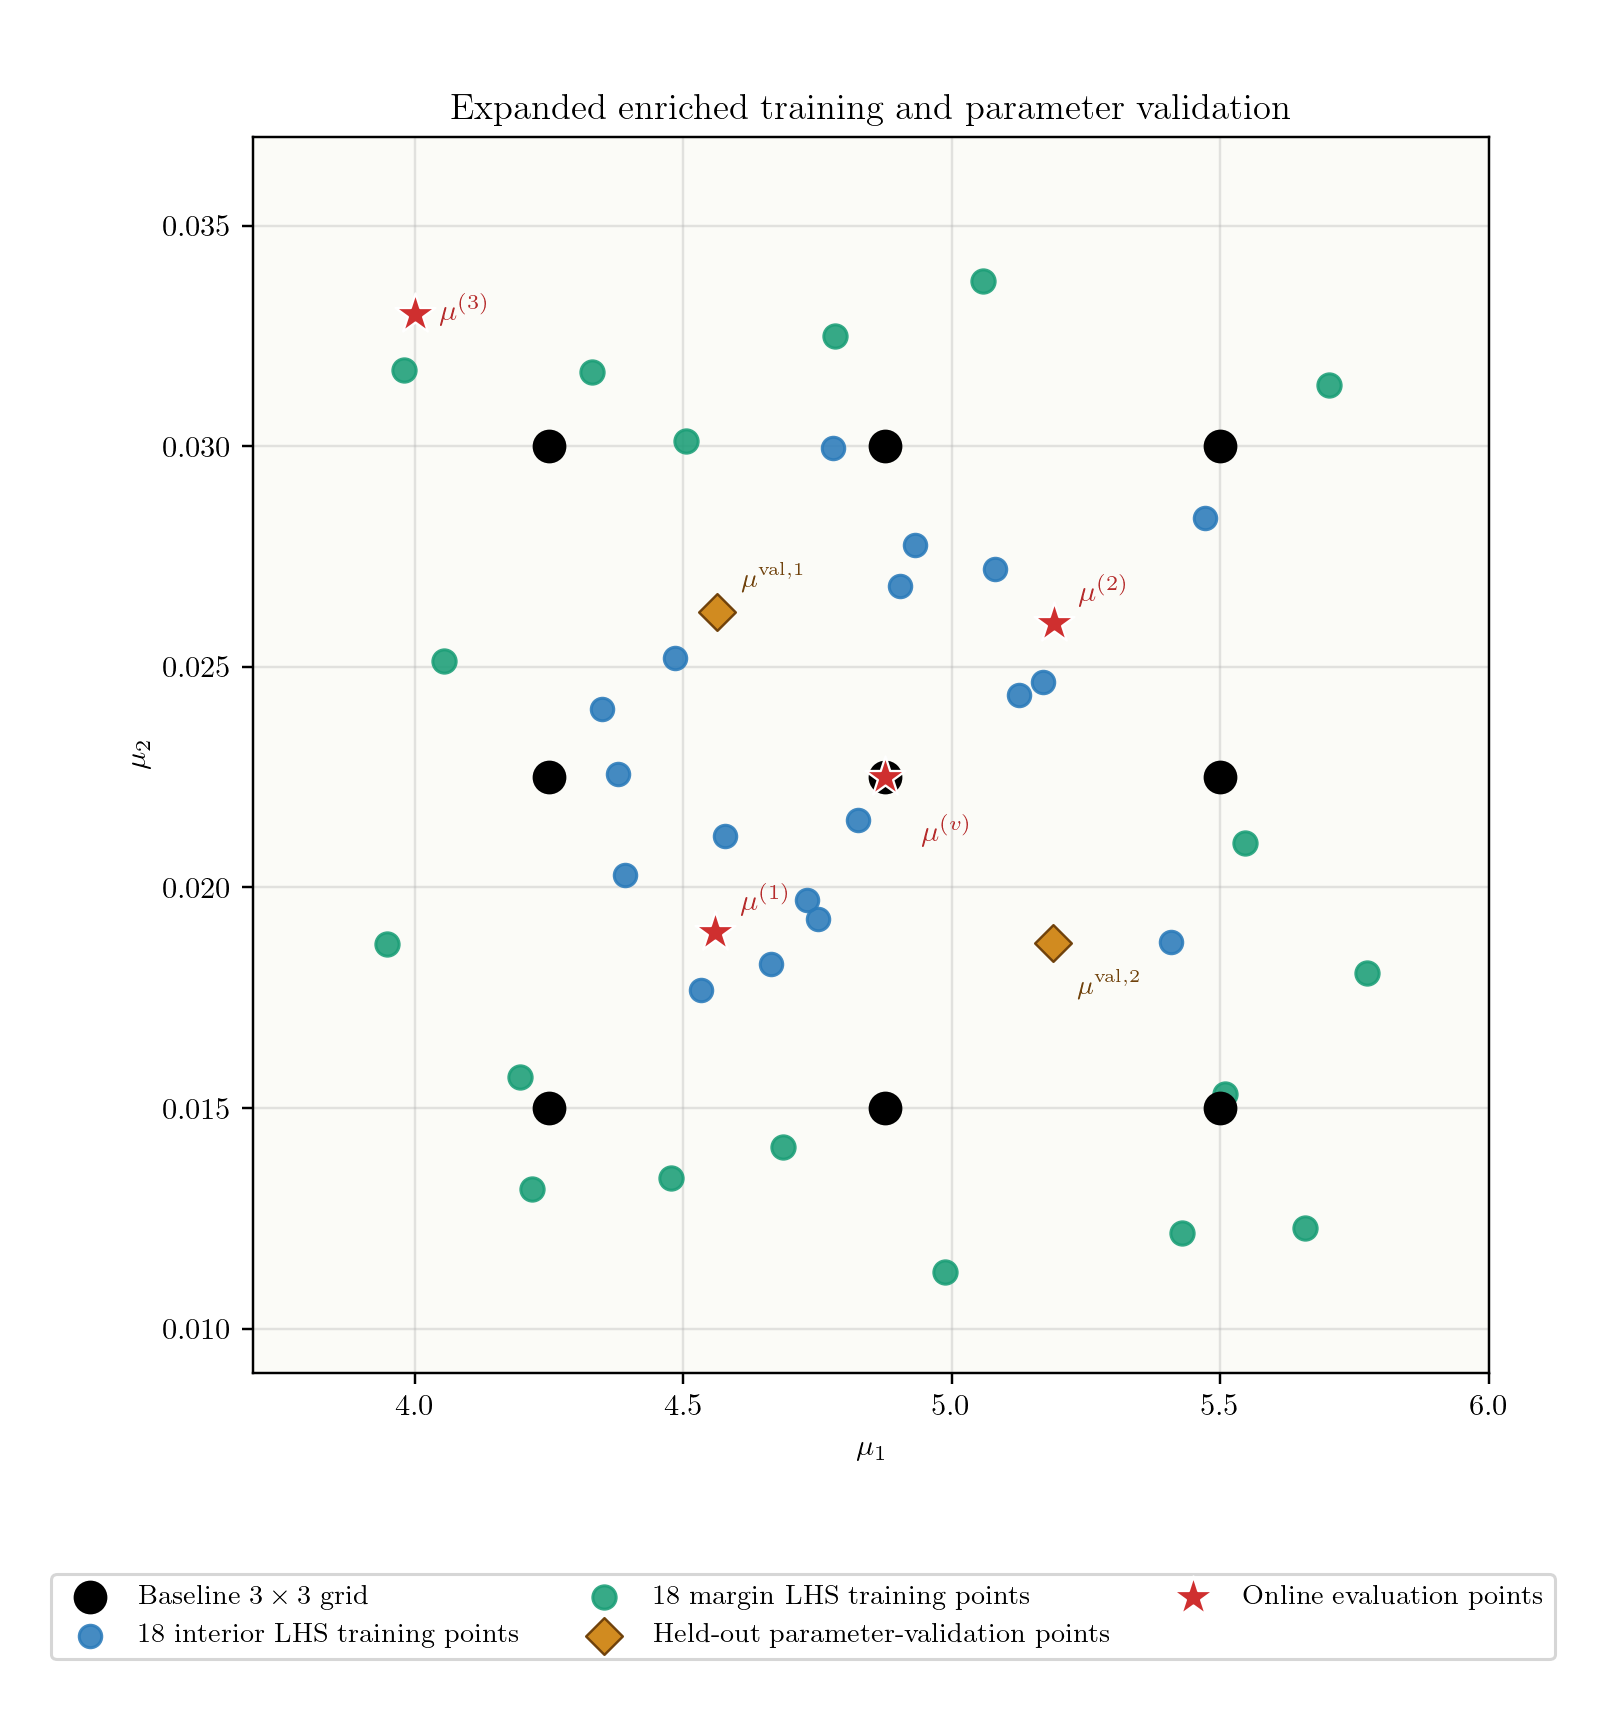
\includegraphics[width=0.74\textwidth]{Figures/prom_only/prom_enrichment_sampling_points.png}
\caption{Expanded enriched training set in parameter space.  The baseline
$3\times3$ grid is supplemented with $18$ interior and $18$ margin
Latin-hypercube points, generated with the fixed linear teacher in the $25\%$
expanded parameter box.  The four evaluation points are excluded from both
training designs.  The axes match Fig.~\ref{fig:enrichment-sampling-baseline};
the enrichment changes coefficient coverage, not the HDM snapshot basis.}
\label{fig:enrichment-sampling-expanded}
\end{figure}

\subsection{PROM and HPROM Evaluation Pipelines}
The PROM and HPROM comparisons are deliberately parallel but not identical.
At the PROM level, the linear teacher and every intrusive learned model use
the full residual.  At the HPROM level, the linear teacher uses its
$151$-coordinate ECM rule and each learned intrusive residual uses a separate
ECM rule matched to its manifold and online unknown dimension.  The reported
nonlinear rules use $2\%$ global parameter--time stratified residual snapshots,
direct dense SVD before ECM, and nonnegative ECM weights.  The direct
POD--NN--ROM and POD--DL--ROM maps do not evaluate a residual and therefore do
not carry an ECM approximation error; they are reported to isolate the
coefficient-learning component.

\subsection{Reported Metrics}
For each evaluation parameter, state accuracy is measured by the relative
space--time error
\begin{equation}
e_u(\bm\mu)=100\,
\frac{\norm{\uvec_{\mathrm{HDM}}-\uvec_{\mathrm{ROM}}}_F}
     {\norm{\uvec_{\mathrm{HDM}}}_F}.
\label{eq:state-error}
\end{equation}
Coefficient diagnostics use the corresponding linear PROM or linear HPROM
trajectory as reference,
\begin{equation}
e_q(\bm\mu)=100\,
\frac{\norm{\q_{151}^{\mathrm{lin}}-\widehat{\q}_{151}}_F}
     {\norm{\q_{151}^{\mathrm{lin}}}_F}.
\label{eq:coefficient-error}
\end{equation}
We report aggregate state and coefficient errors, per-index coefficient
errors, and solution overlays.  The linear reference is an accuracy benchmark
for the fixed trial space and residual level, not a theorem-level lower bound
against the HDM.


% Current, reproducible PROM and HPROM results.

\section{Baseline PROM-Only Results}
Table~\ref{tab:prom-training} reports the selected baseline training runs.  The largest validation error occurs for
the master parameter--time map because it predicts all 151 coefficients from only \((\mu_1,\mu_2,t)\).  The Case 1,
Case 3, and autoencoder tasks are easier because their inputs contain coefficient information.

\begin{table}[H]
\centering
\caption{Baseline PROM-only Stage--3 selected networks.  Errors are relative Frobenius percentages in coefficient space.}
\label{tab:prom-training}
\resizebox{\textwidth}{!}{\begin{tabular}{llrrr}
\toprule
Model & learned map & parameters & train (\%) & validation (\%) \\
\midrule
PROM--ANN Case 1 & $(q_1,\ldots,q_{10})\mapsto(q_{11},\ldots,q_{151})$ & 564,621 & 1.130 & 1.251 \\
PROM--ANN Case 3 & $(q_1,\ldots,q_{10},\mu_1,\mu_2,t)\mapsto(q_{11},\ldots,q_{151})$ & 565,389 & 0.405 & 0.482 \\
Master POD--NN--ROM (Case 2 tail source) & $(\mu_1,\mu_2,t)\mapsto(q_1,\ldots,q_{151})$ & 565,399 & 2.601 & 4.391 \\
PROM--POD--AE & $q_{1:151}\mapsto z_{1:10}\mapsto q_{1:151}$ & 486,817 & 0.106 & 0.127 \\
POD--DL--ROM & $(\mu_1,\mu_2,t)\mapsto z_{1:10}\mapsto q_{1:151}$ & 952,747 & 0.810 & 0.935 \\
\bottomrule
\end{tabular}
}
\end{table}

Table~\ref{tab:prom-online} gives the baseline online state error.  The linear PROM is not a theorem-level lower
bound against the HDM, but it is the reference accuracy level associated with the fixed \(151\)-dimensional PROM
basis and teacher data.  The intrusive learned PROMs are close to that reference for in-domain points.  The purely
non-intrusive maps degrade more strongly, especially at the extrapolatory point.

\begin{table}[H]
\centering
\caption{Baseline PROM-only online errors
\(100\norm{\uvec_{\mathrm{HDM}}-\uvec_{\mathrm{ROM}}}_F/\norm{\uvec_{\mathrm{HDM}}}_F\).  The mean column averages
\(\mub^{(v)},\mub^{(1)},\mub^{(2)}\).}
\label{tab:prom-online}
\resizebox{\textwidth}{!}{\begin{tabular}{lrrrrr}
\toprule
Model & $\mu^{(v)}$ & $\mu^{(1)}$ & $\mu^{(2)}$ & Mean & $\mu^{(3)}$ \\
\midrule
Linear PROM & 0.413 & 0.460 & 0.472 & 0.448 & 0.868 \\
PROM--ANN Case 1 & 0.409 & 0.520 & 0.683 & 0.537 & 1.584 \\
PROM--ANN Case 2 ($n=10$) & 1.013 & 1.427 & 1.670 & 1.370 & 1.898 \\
PROM--ANN Case 2 ($n=20$) & 0.999 & 1.328 & 1.505 & 1.278 & 1.658 \\
PROM--ANN Case 3 & 0.405 & 0.521 & 0.576 & 0.501 & 1.392 \\
PROM--POD--AE ($n_z=10$) & 0.408 & 0.539 & 0.607 & 0.518 & 1.978 \\
\midrule
POD--NN--ROM & 1.036 & 1.675 & 1.842 & 1.518 & 3.214 \\
POD--DL--ROM ($n_z=10$) & 0.489 & 1.398 & 1.463 & 1.116 & 3.728 \\
\bottomrule
\end{tabular}
}
\end{table}

\begin{figure}[H]
\centering
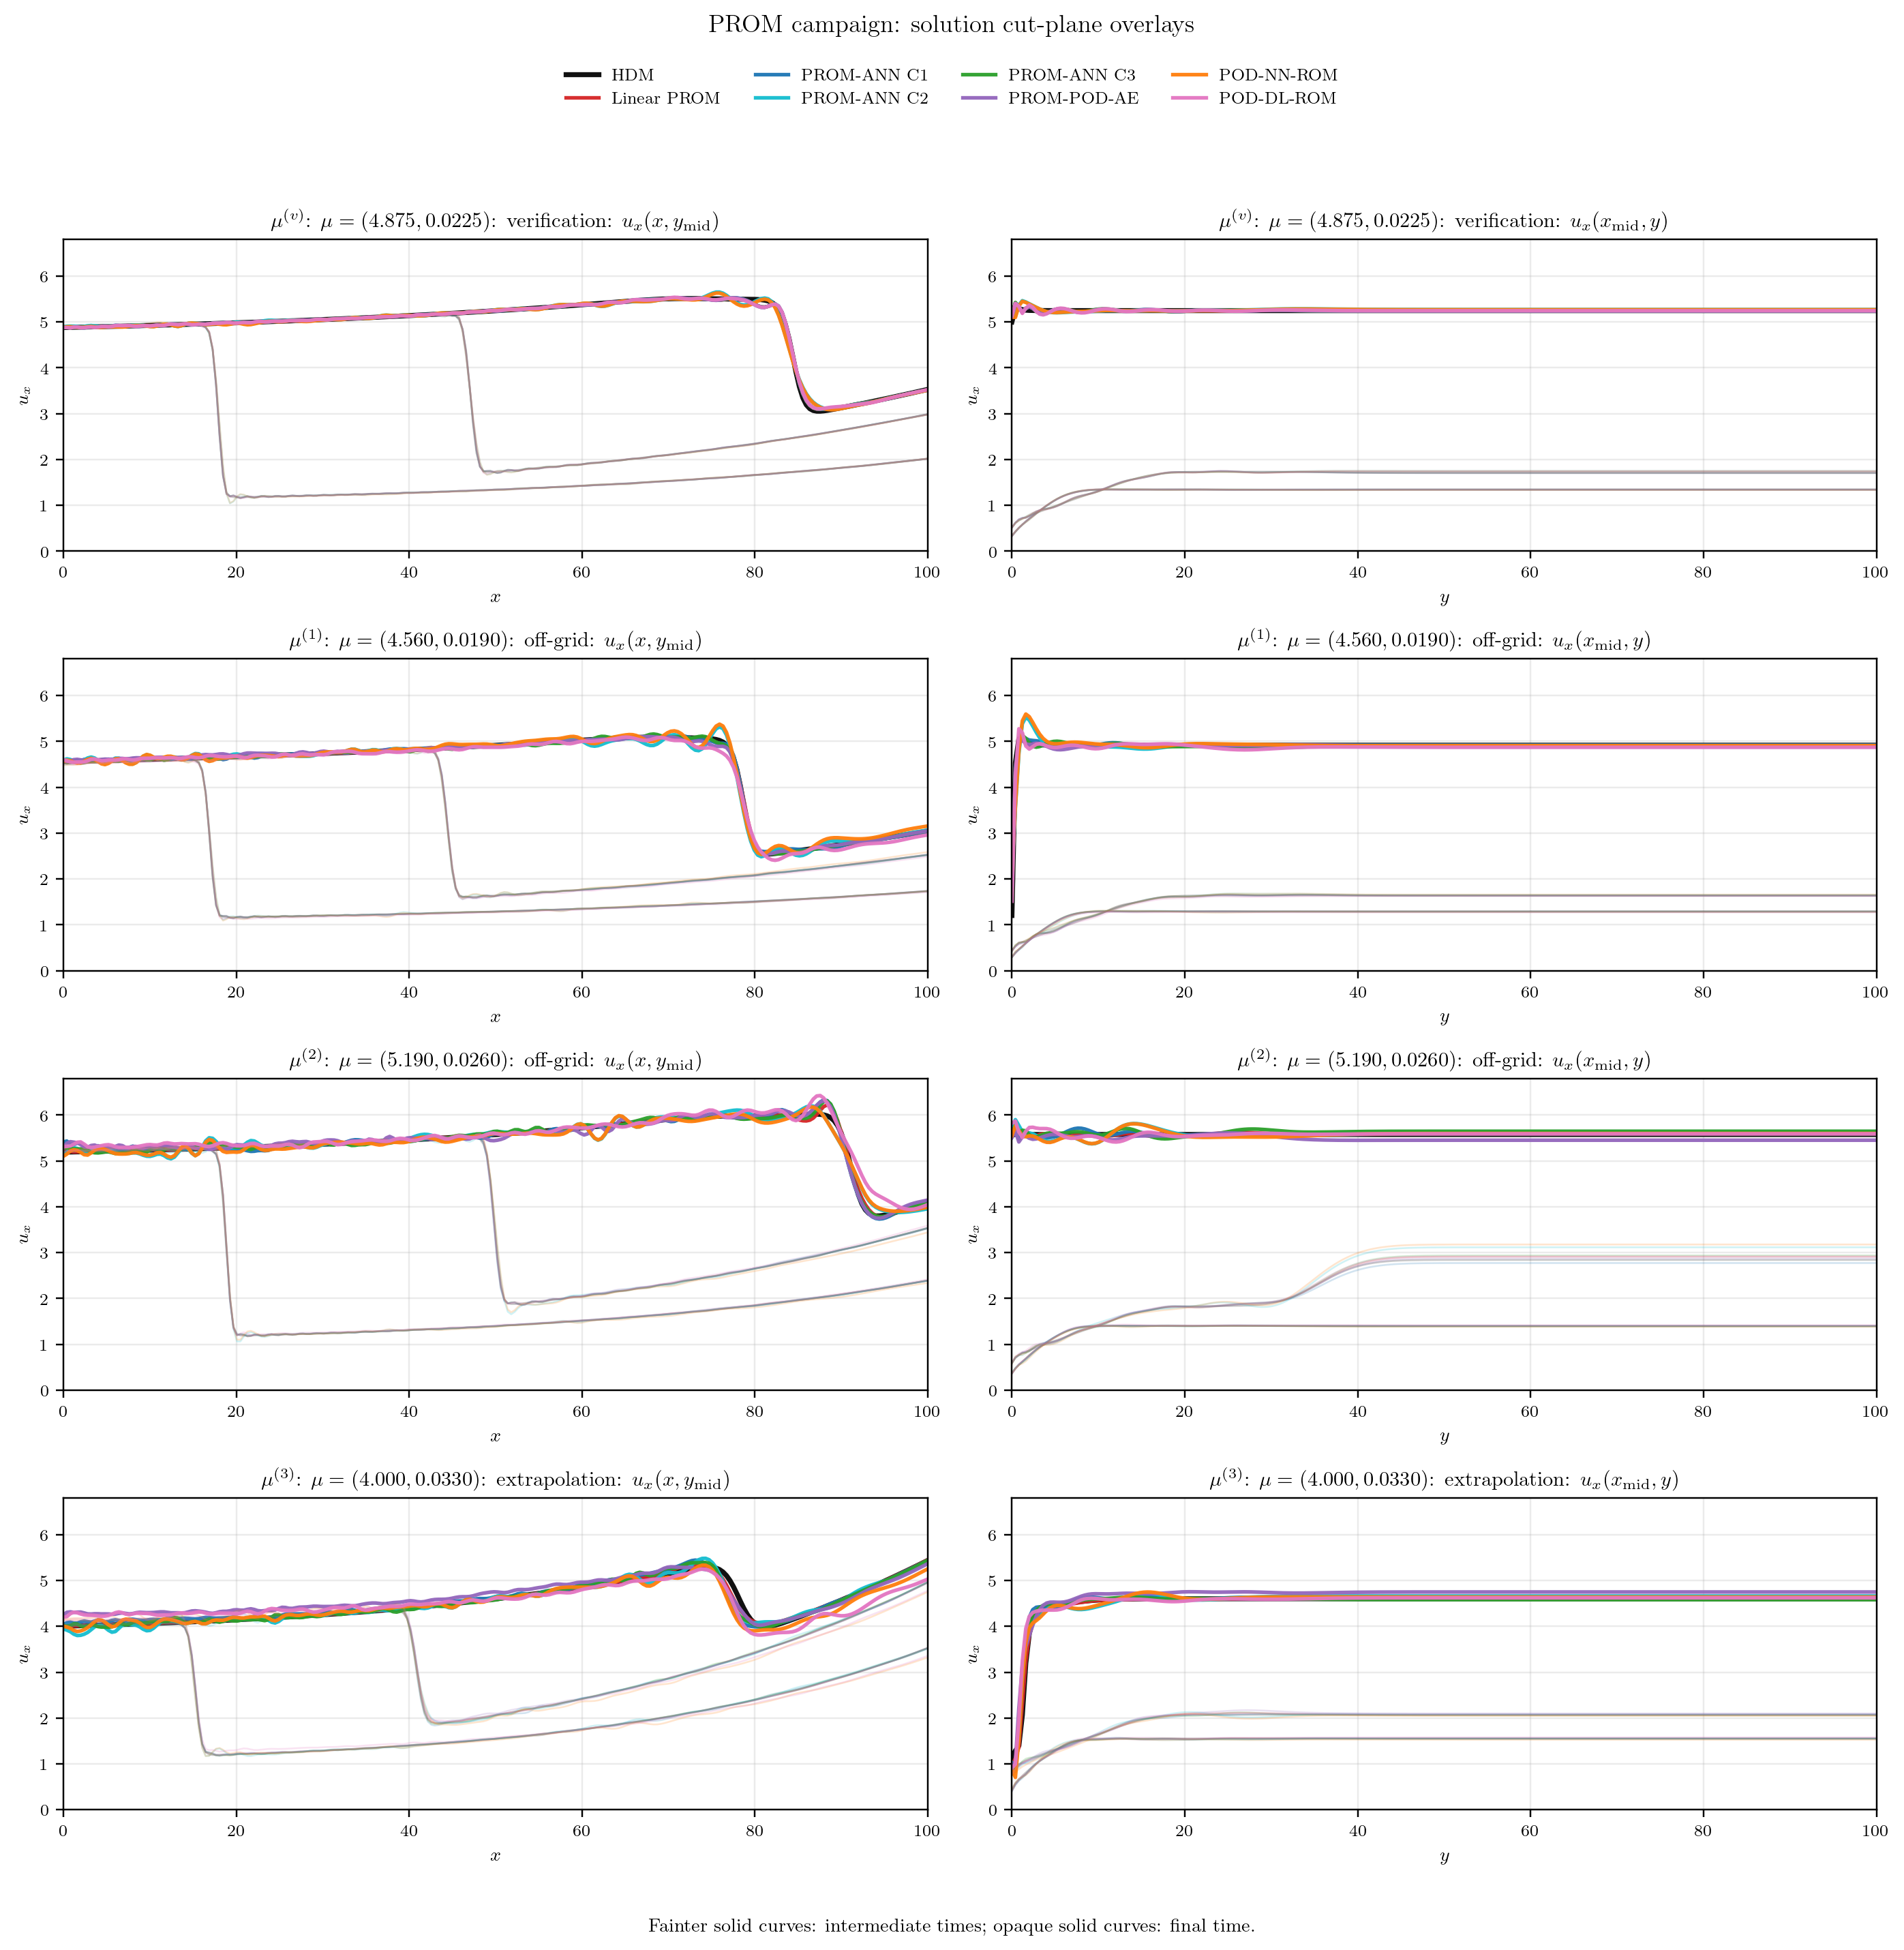
\includegraphics[width=0.98\textwidth]{Figures/prom_only/prom_only_solution_overlays.png}
\caption{Baseline PROM solution cut-plane comparison against the HDM at the four evaluation points.  Each row
corresponds to one parameter, with $u_x(x,y_{\mathrm{mid}})$ at left and $u_x(x_{\mathrm{mid}},y)$ at right.
Fainter solid curves denote the two intermediate times and opaque solid curves the final time.  All panels use the same
vertical range for $u_x$, so the visible deviations are directly comparable across parameters and cut planes.}
\label{fig:prom-solution-overlays}
\end{figure}

\section{Baseline Online Coefficient Diagnostics}
The online state error is the final metric, but coefficient-space diagnostics explain where the learned models lose
accuracy.  Table~\ref{tab:prom-online-coeff} reports coefficient errors from the actual online outputs.  Case 1,
Case 2, Case 3, and PROM--POD--AE use their PROM online trajectories, while POD--NN--ROM and POD--DL--ROM use their
direct non-intrusive predictions.  All coefficient errors are measured against the linear PROM trajectory with
\(n_{\mathrm{tot}}=151\).  For Case 1 and Case 3, the online solver did not save \(\q(t)\) directly, so the
coefficients are recovered from the saved PROM state snapshots by
\begin{equation}
  \q(t)=\arg\min_{\eta\in\mathbb R^{151}}
  \left\lVert \V_{151}\eta-\left(\uvec_{\mathrm{PROM}}(t)-\uvec_{\mathrm{ref}}\right)\right\rVert_2 .
\end{equation}

\begin{table}[H]
\centering
\caption{Baseline online coefficient error against the linear PROM with \(n_{\mathrm{tot}}=151\).  Values are
relative Frobenius percentages over all 151 coefficients and all time steps.}
\label{tab:prom-online-coeff}
\resizebox{0.9\textwidth}{!}{\begin{tabular}{lrrrrr}
\toprule
Model & $\mu^{(v)}$ & $\mu^{(1)}$ & $\mu^{(2)}$ & Mean & $\mu^{(3)}$ \\
\midrule
Linear PROM & 0.000 & 0.000 & 0.000 & 0.000 & 0.000 \\
PROM--ANN Case 1 & 0.295 & 0.593 & 1.297 & 0.729 & 2.923 \\
PROM--ANN Case 2 ($n=10$) & 2.440 & 3.361 & 3.906 & 3.236 & 4.257 \\
PROM--ANN Case 2 ($n=20$) & 2.401 & 3.123 & 3.512 & 3.012 & 3.662 \\
PROM--ANN Case 3 & 0.164 & 0.856 & 0.788 & 0.603 & 2.396 \\
PROM--POD--AE & 0.140 & 0.773 & 0.929 & 0.614 & 4.394 \\
\midrule
POD--NN--ROM & 2.499 & 3.924 & 4.249 & 3.557 & 7.444 \\
POD--DL--ROM & 0.814 & 3.129 & 3.225 & 2.389 & 8.639 \\
\bottomrule
\end{tabular}
}
\end{table}

\begin{figure}[H]
\centering
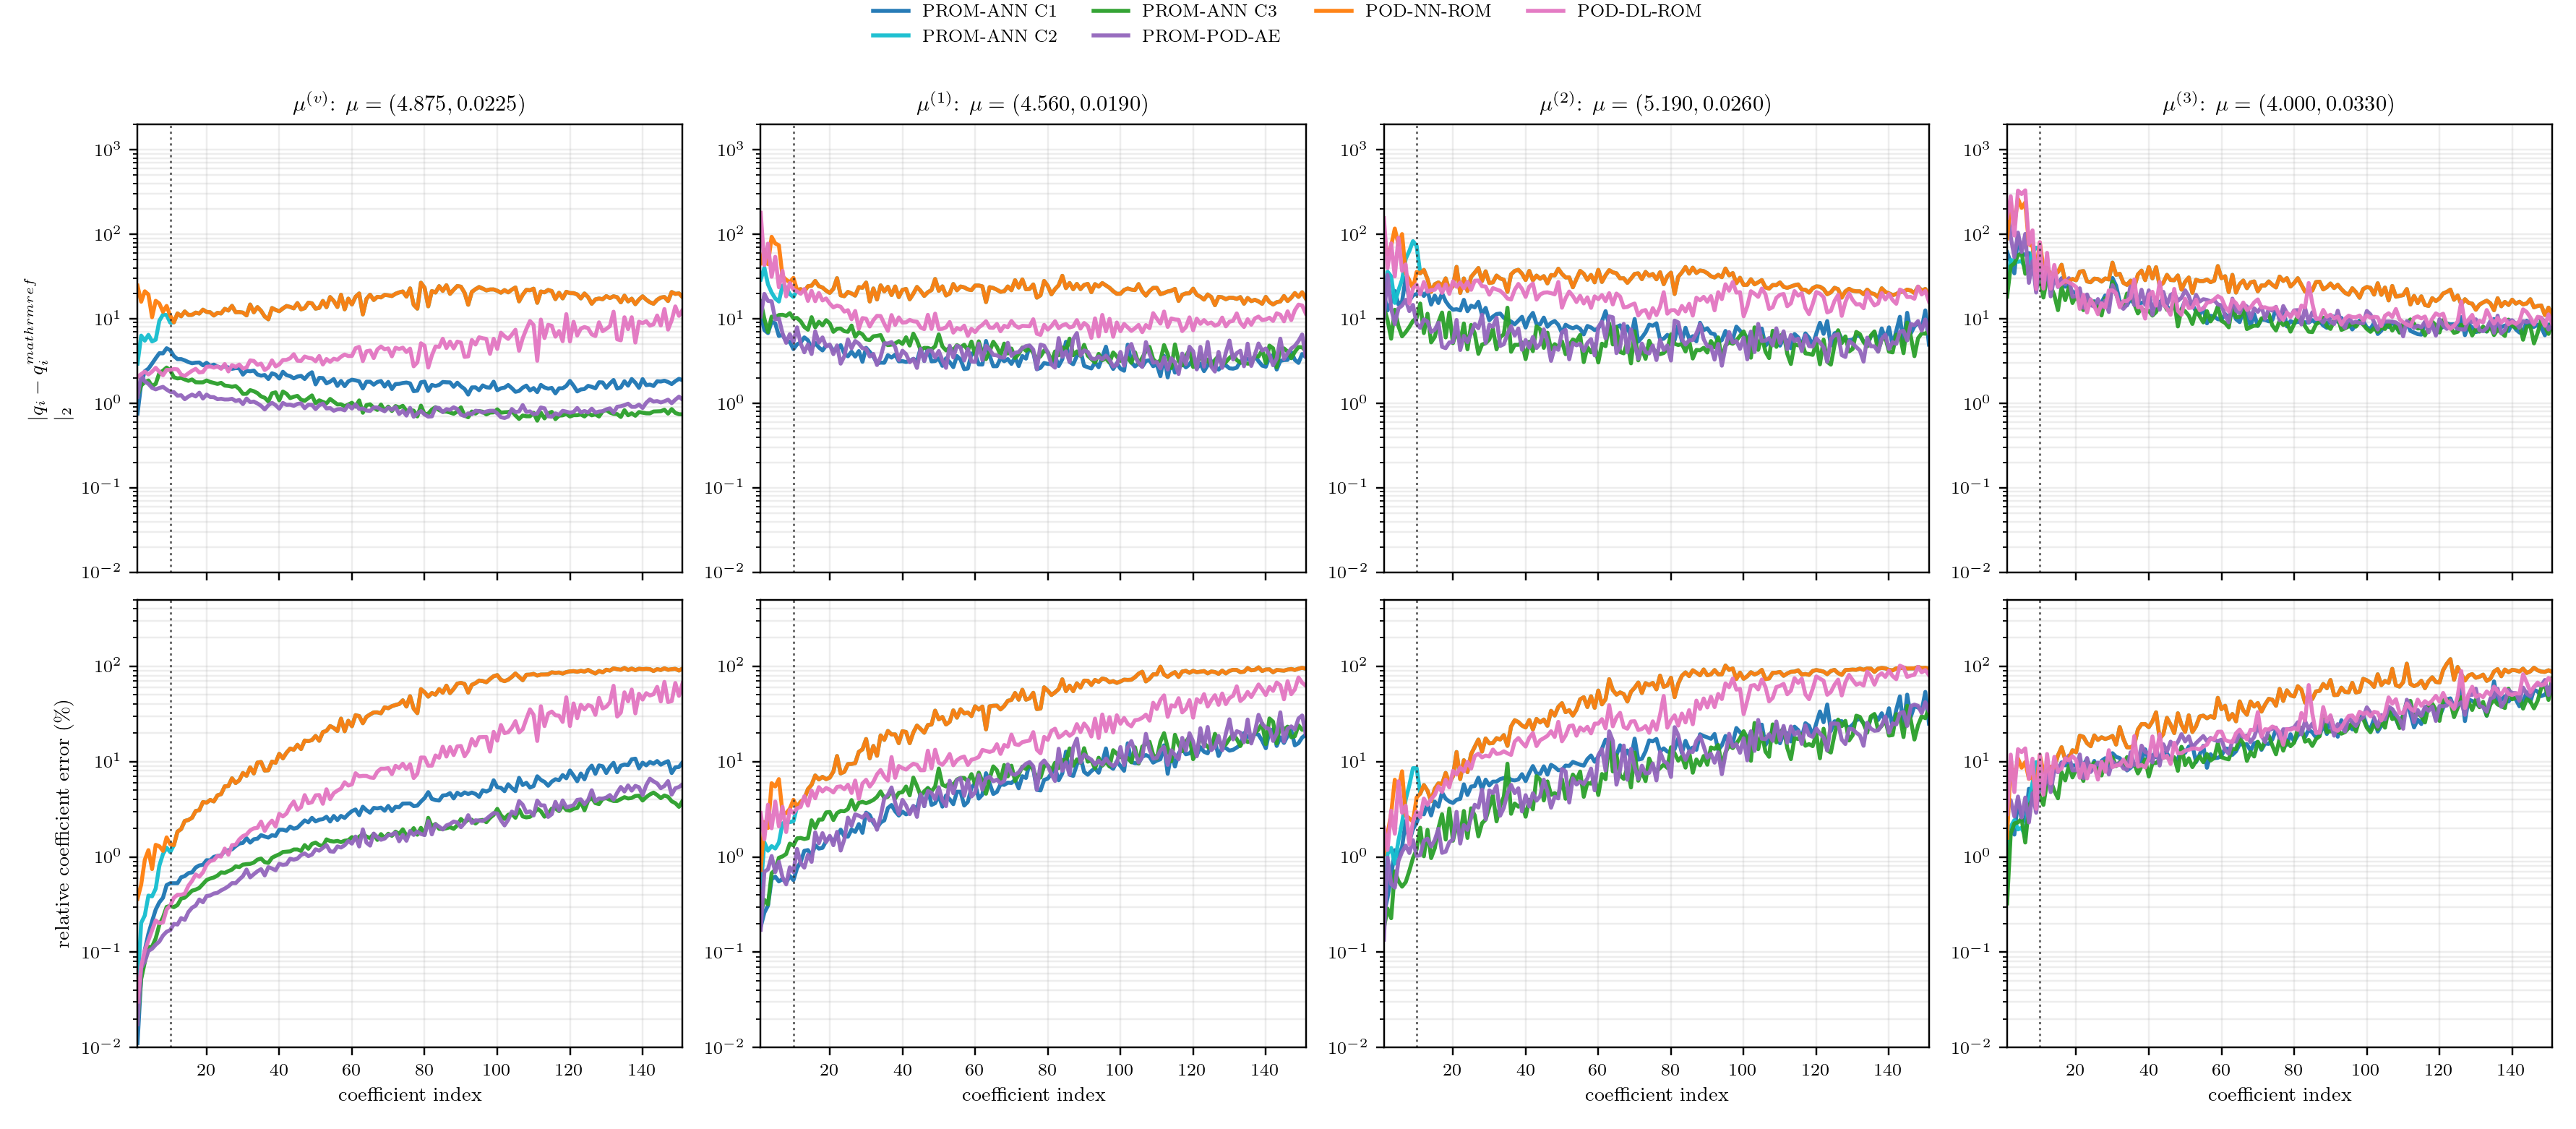
\includegraphics[width=0.98\textwidth]{Figures/prom_only/prom_only_coeff_abs_rel_errors.png}
\caption{Baseline online coefficient errors against the \(n_{\mathrm{tot}}=151\) linear PROM trajectory.  Top:
absolute trajectory error \(\lVert q_i-q_i^{\mathrm{ref}}\rVert_2\). Bottom: the same error relative to
\(\lVert q_i^{\mathrm{ref}}\rVert_2\), reported as a percentage.  All columns in each row use the same logarithmic
ordinate limits, and the vertical line marks coefficient 10.  The linear PROM itself is the reference and is not plotted.}
\label{fig:prom-coeff-rel-errors}
\end{figure}

The high-index coefficients often show large relative errors because their trajectory norms are small.  This does
not mean that each high-index coefficient dominates the state error.  It does show, however, that the map
\((\mu_1,\mu_2,t)\mapsto\q_{151}\) is data-limited in the baseline regime: the high-index tail is low energy but
still difficult to interpolate from only nine parameter trajectories.

\begin{figure}[H]
\centering
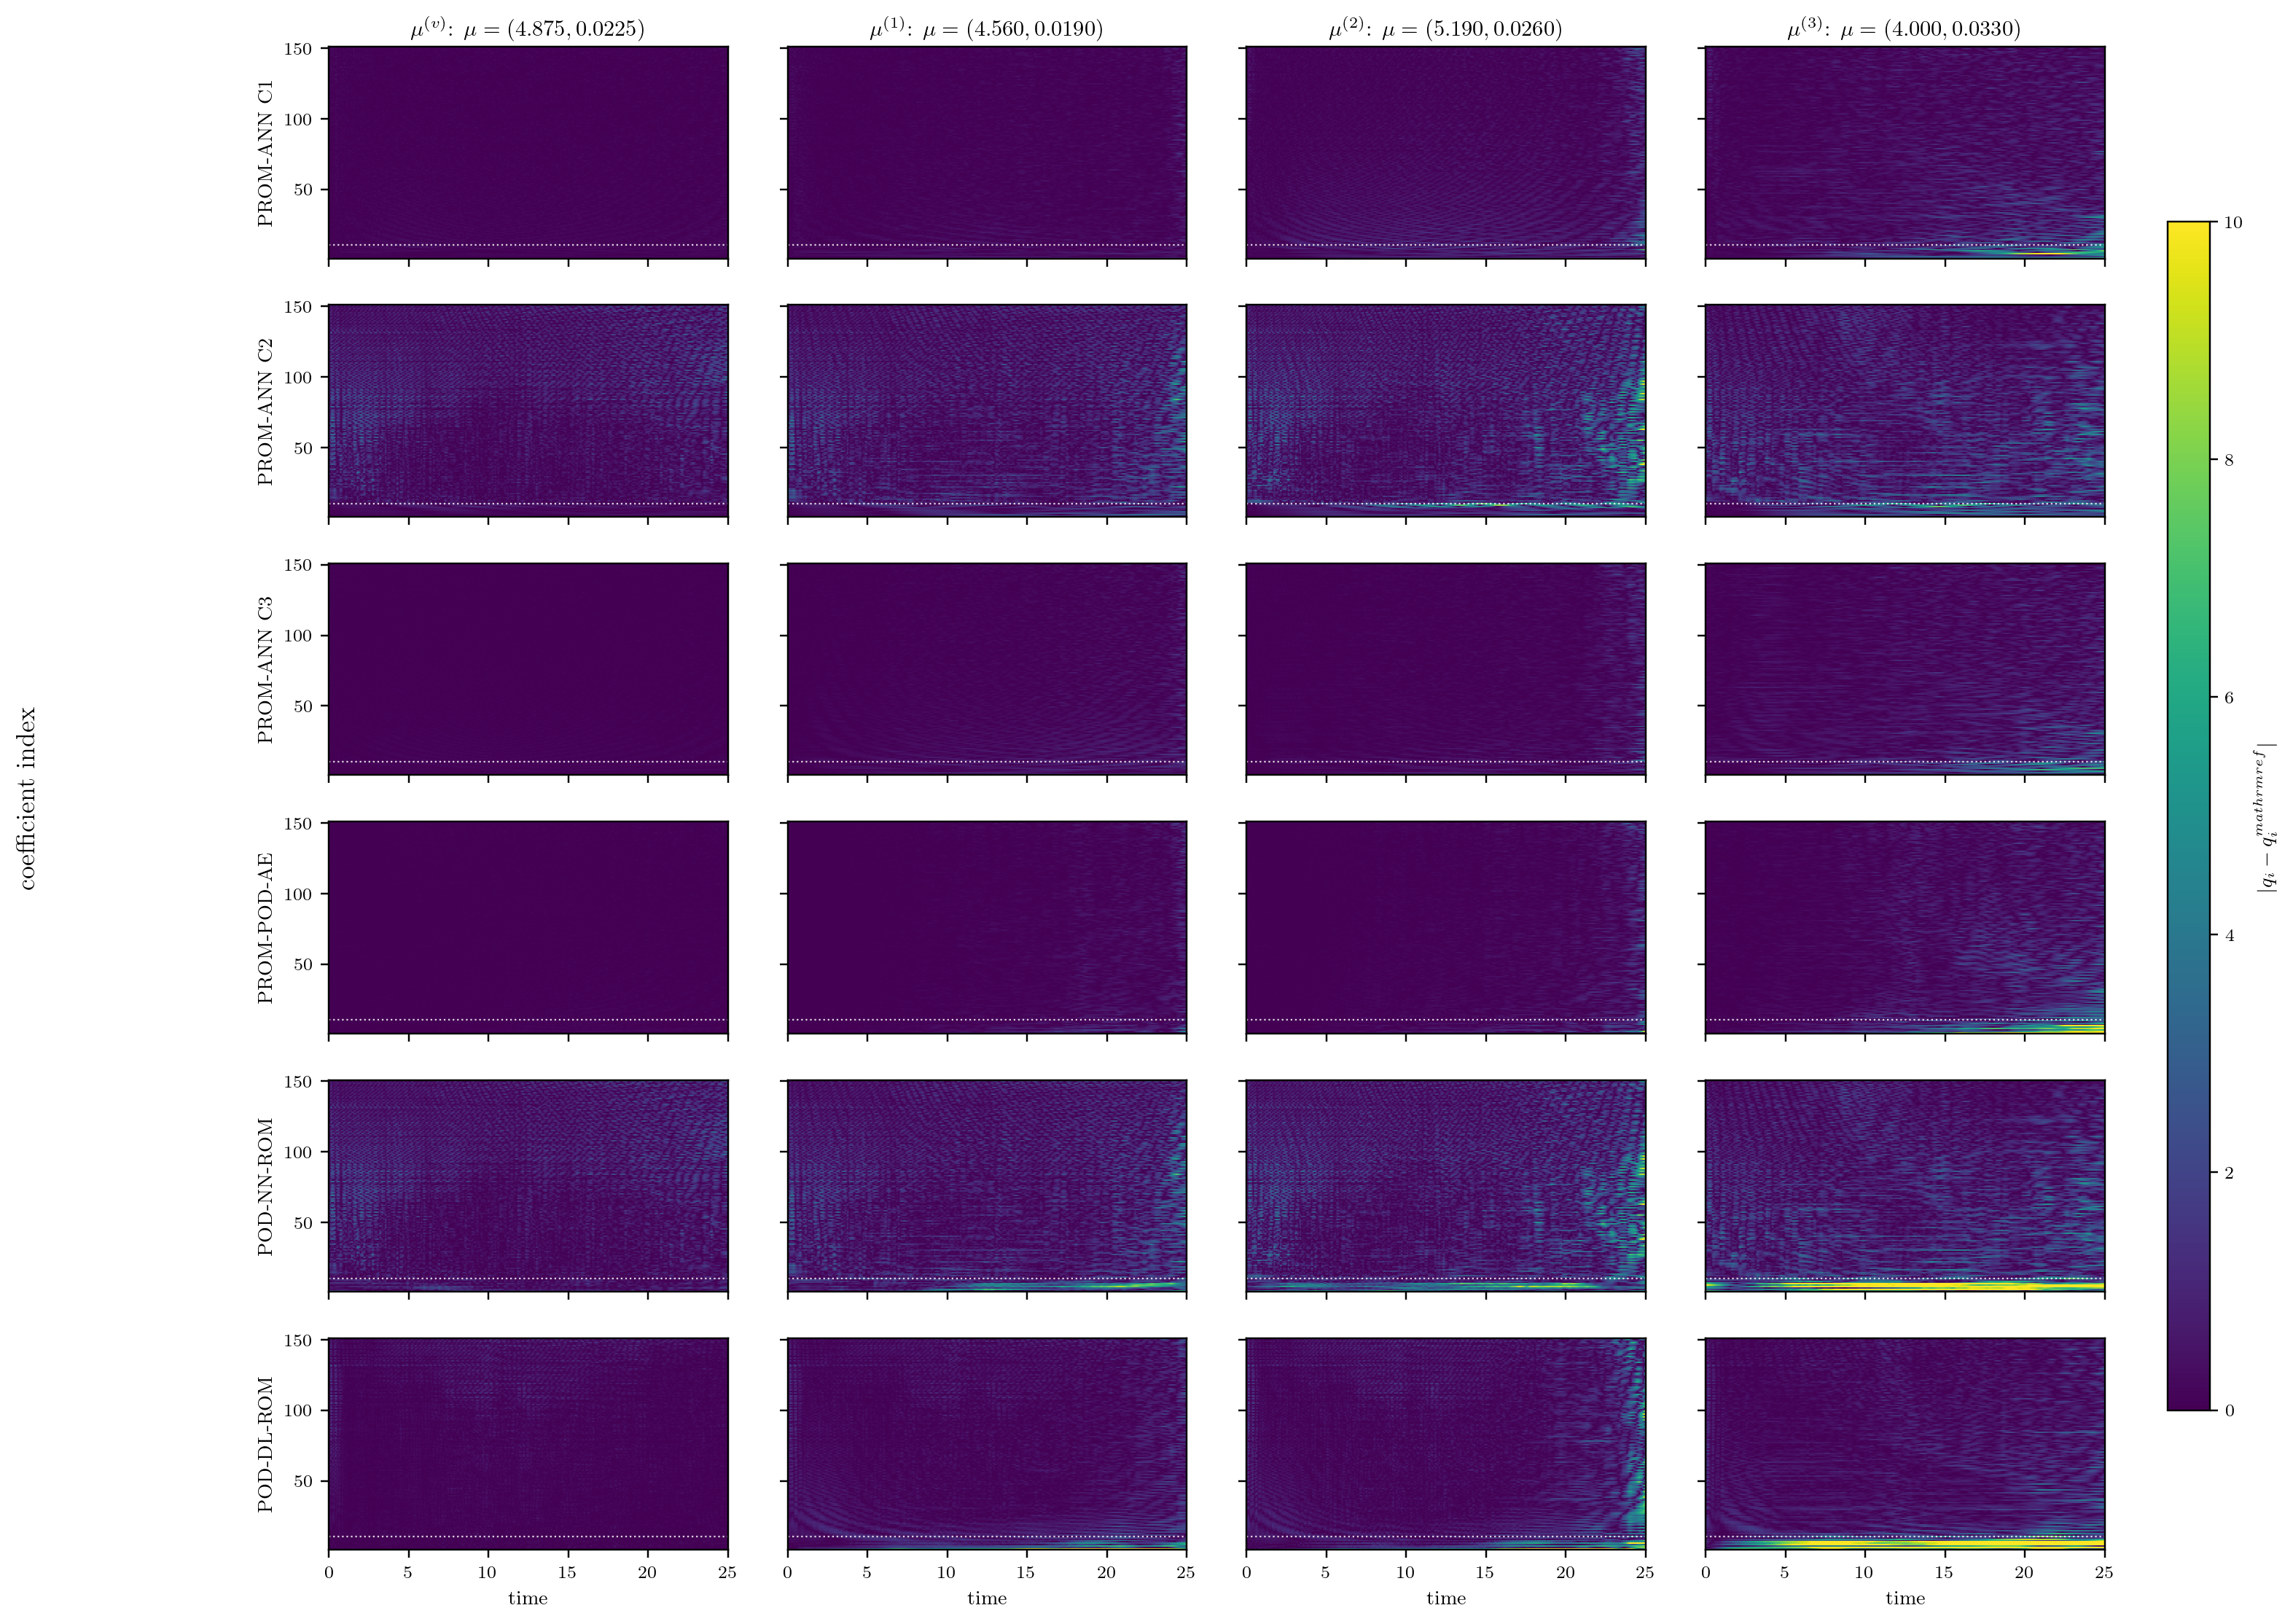
\includegraphics[width=0.98\textwidth]{Figures/prom_only/prom_only_coeff_abs_heatmaps.png}
\caption{Baseline PROM time-by-coefficient absolute errors \(\lvert q_i(t)-q_i^{\mathrm{ref}}(t)\rvert\) against the
linear PROM.  Columns are ordered as \(\mub^{(v)}\), \(\mub^{(1)}\), \(\mub^{(2)}\), and \(\mub^{(3)}\); rows identify
the online model.  The dotted horizontal line is the ten-coordinate primary/secondary split.  One common colourbar
is used for every panel.}
\label{fig:prom-coeff-abs-heatmaps}
\end{figure}

\begin{figure}[H]
\centering
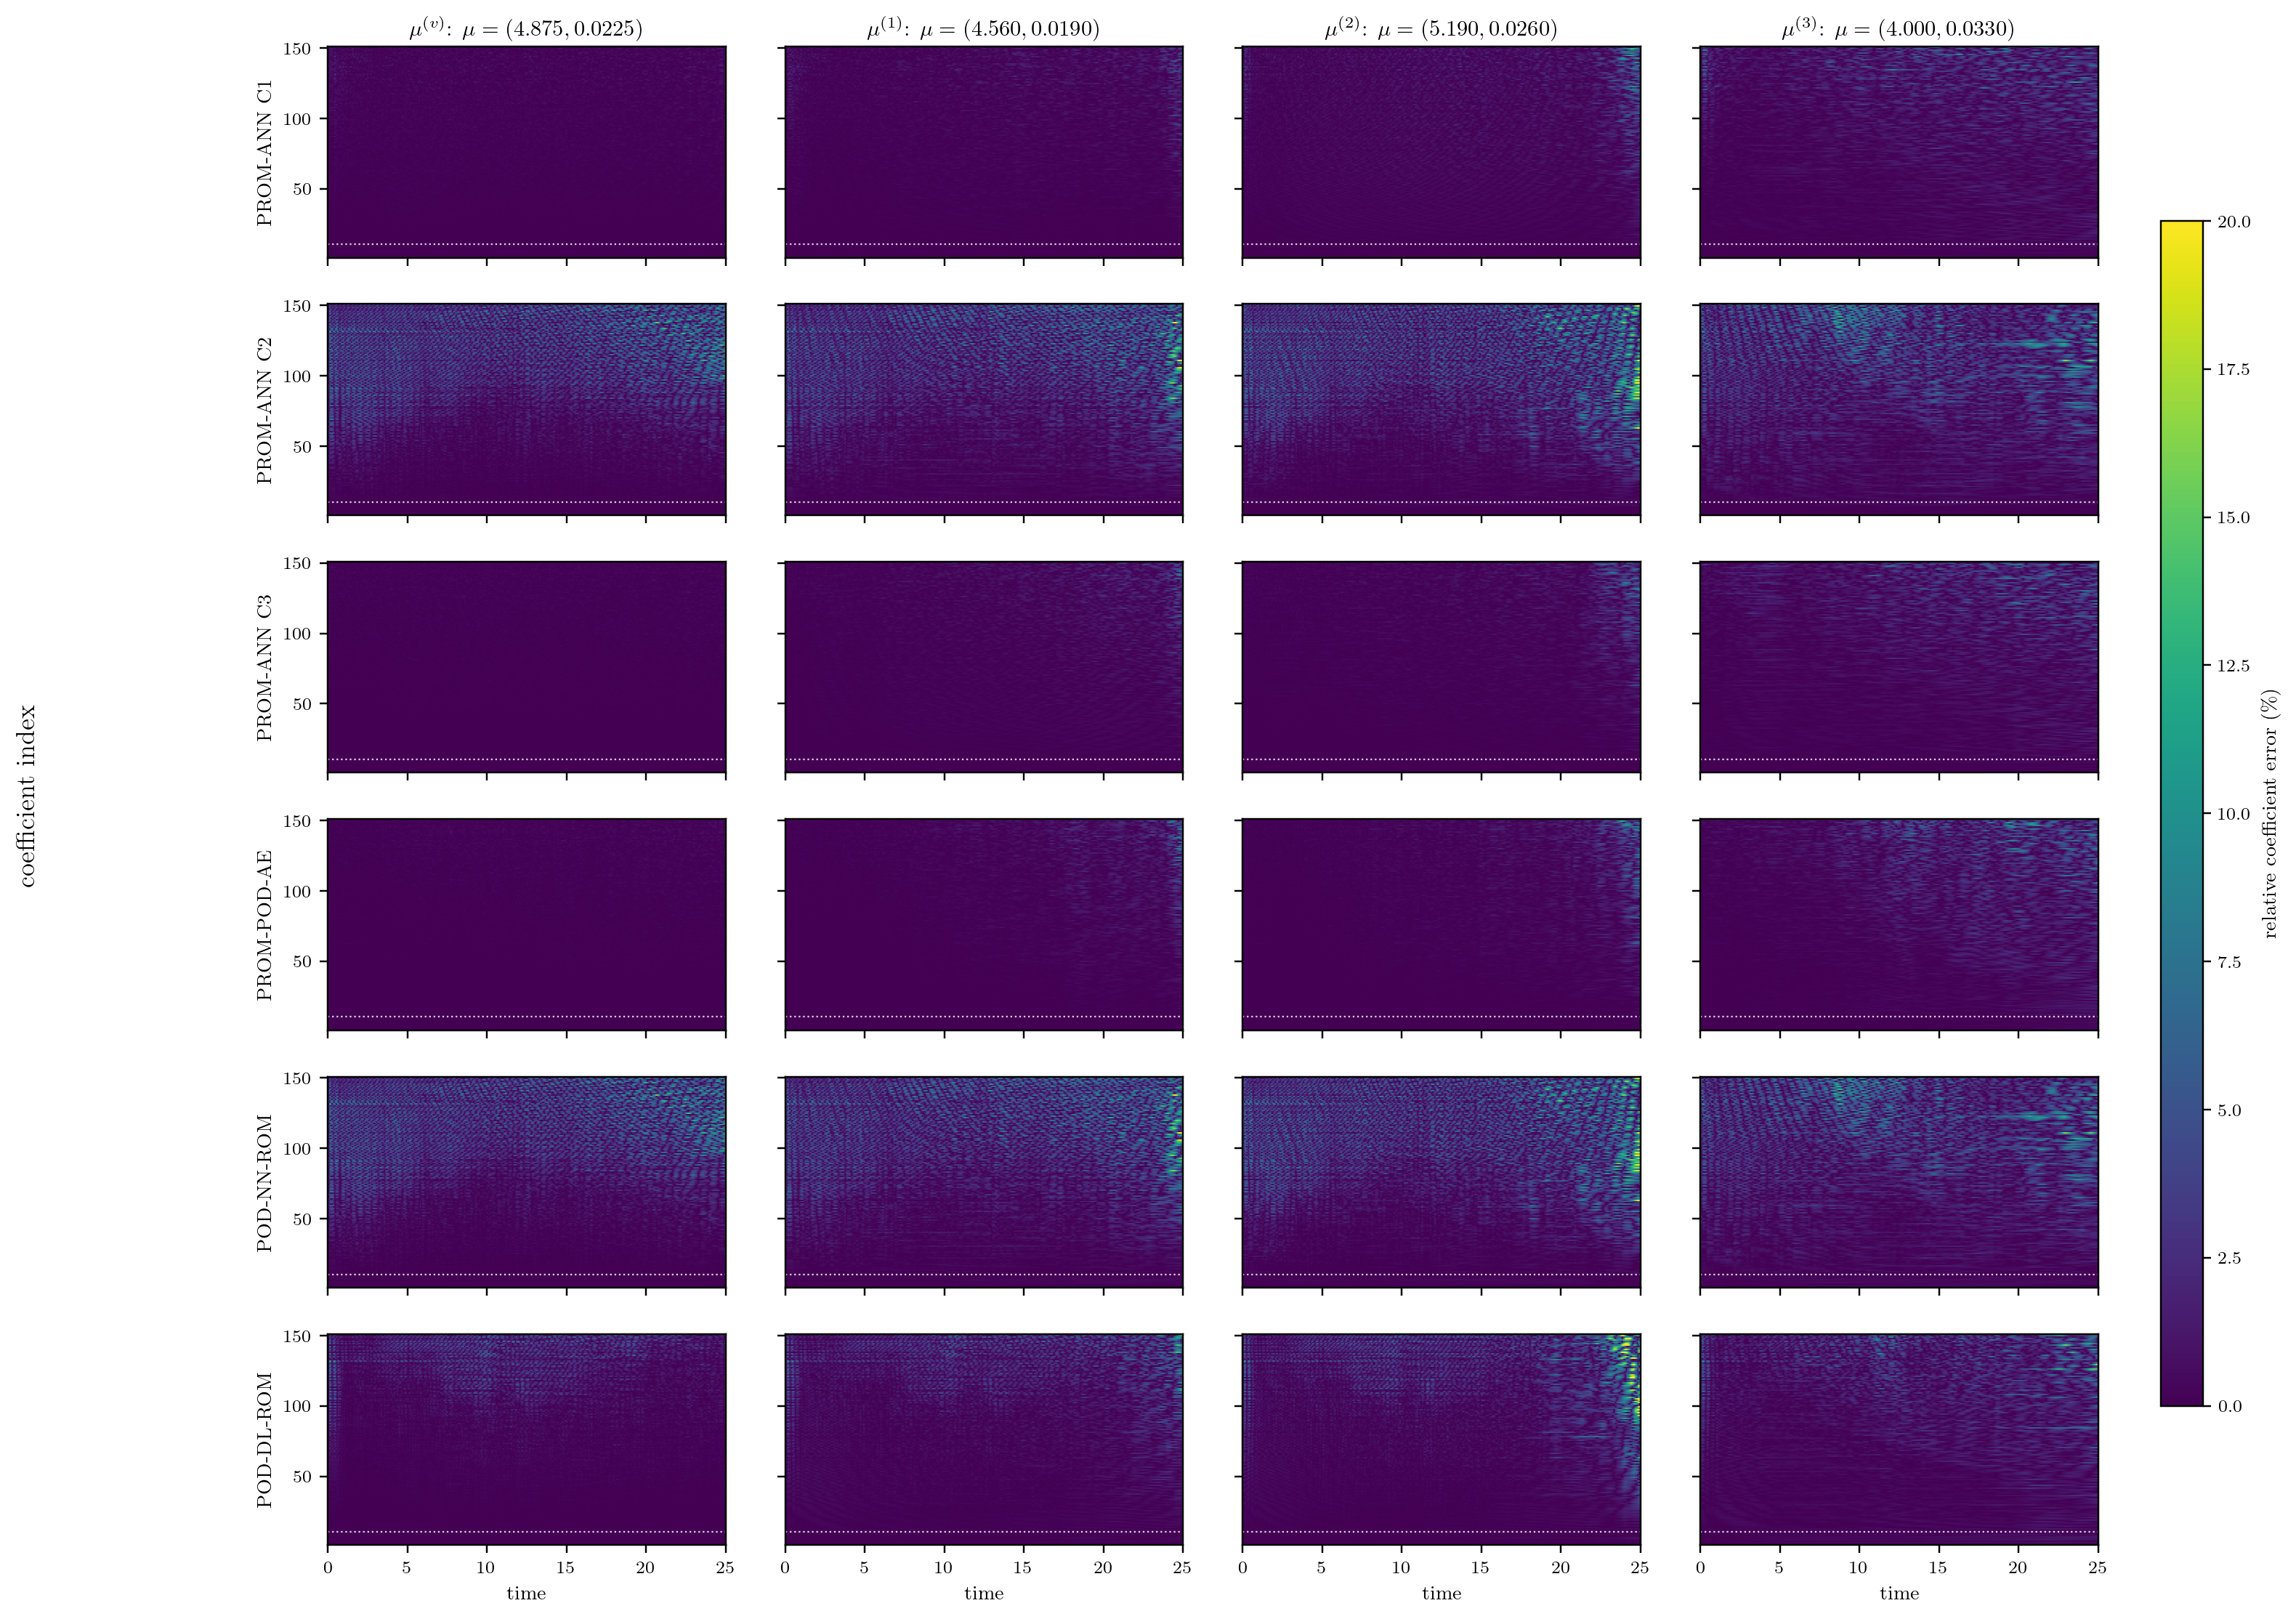
\includegraphics[width=0.98\textwidth]{Figures/prom_only/prom_only_coeff_rel_heatmaps.png}
\caption{Baseline PROM time-by-coefficient relative errors, using
\(100\lvert q_i(t)-q_i^{\mathrm{ref}}(t)\rvert/\lVert q_i^{\mathrm{ref}}\rVert_2\).  The colour range is fixed for all
PROM and HPROM heatmaps; values above \(20\%\) are shown at the upper colour limit so that lower-error structure
remains visible.}
\label{fig:prom-coeff-rel-heatmaps}
\end{figure}

\subsection{Case--2 PROM Diagnostic Sweep}
Case 2 connects the direct parameter--time map to the full linear PROM.  We run
\begin{equation}
  n\in\{0,3,5,10,20,30,50,100,151\},
\end{equation}
where \(n=0\) is exactly the POD--NN--ROM prediction from the shared master network and \(n=151\) is the linear
PROM.  For intermediate \(n\), LSPG solves the first \(n\) coordinates while the same master ANN supplies the
remaining coordinates.

\begin{figure}[H]
\centering
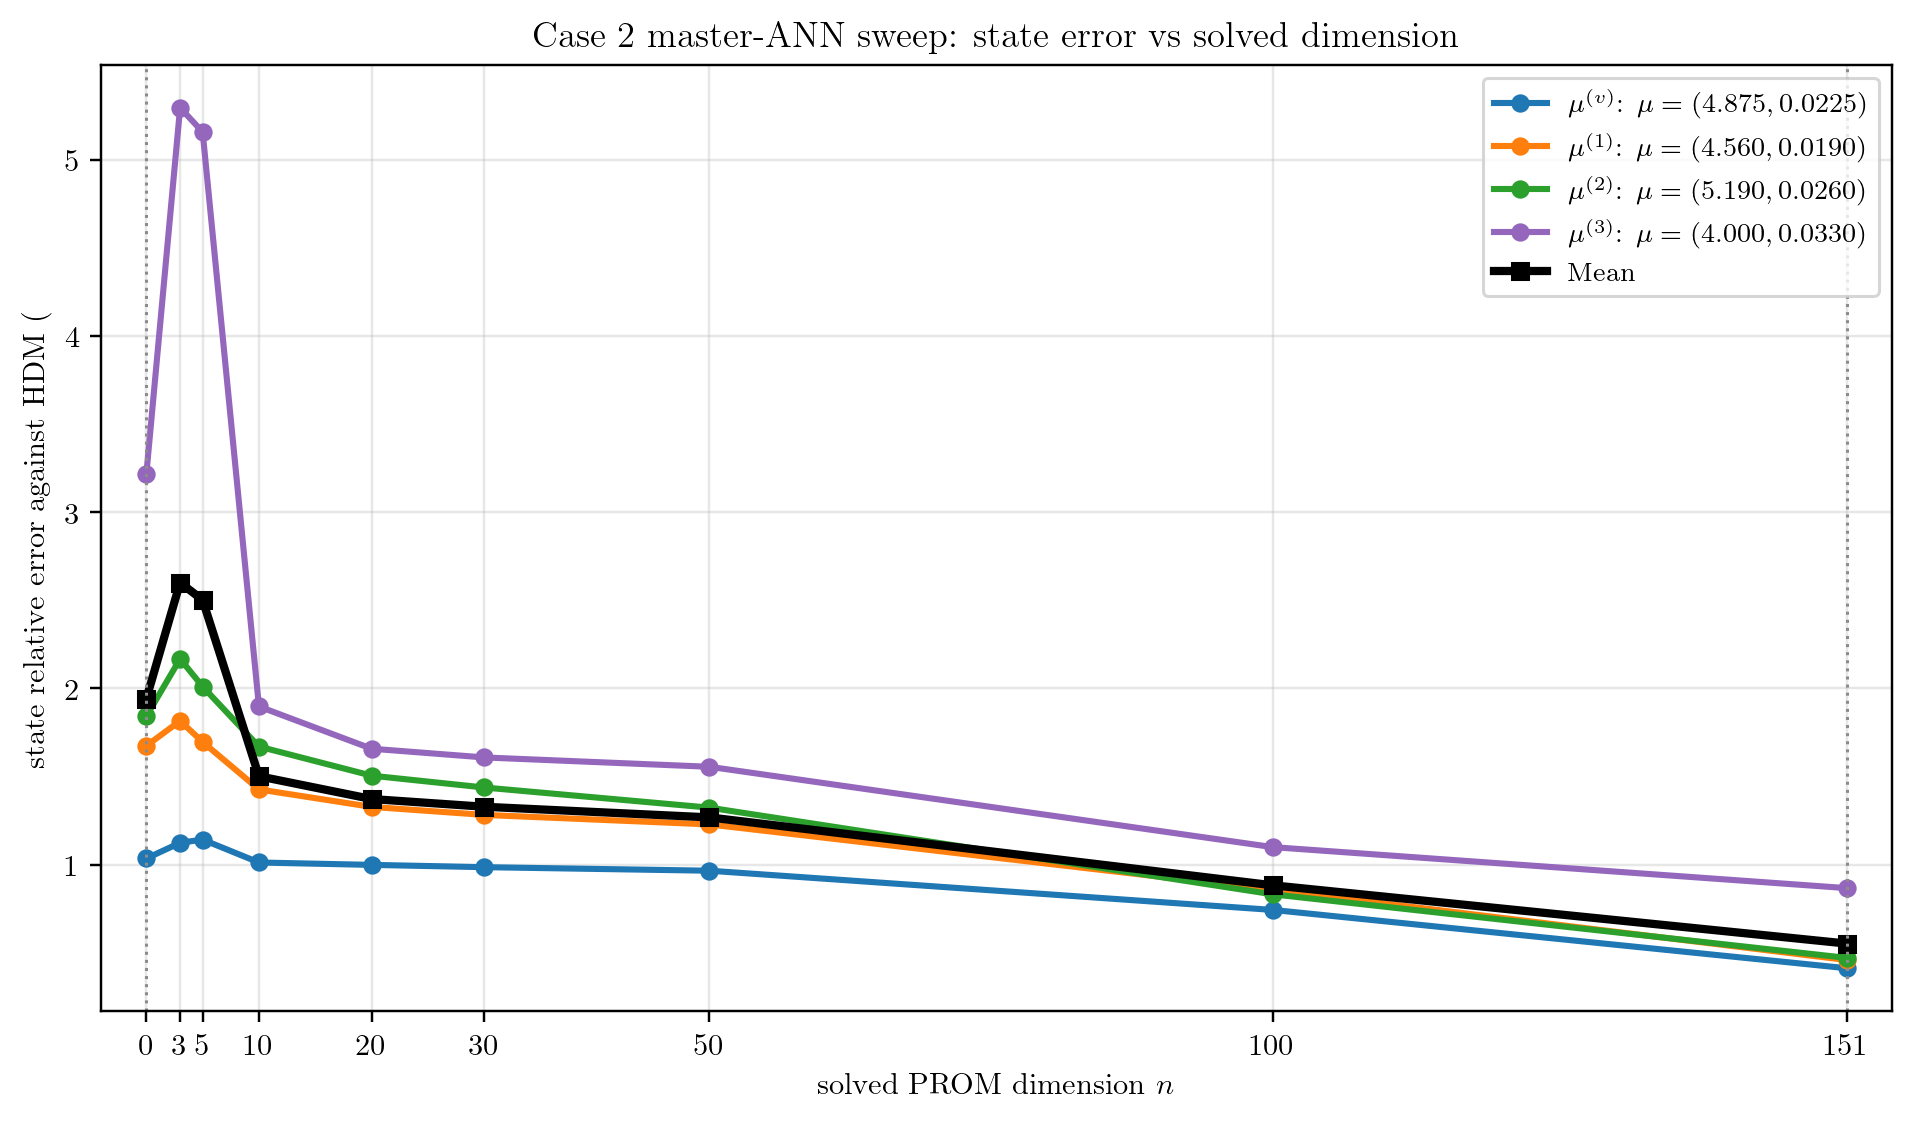
\includegraphics[width=0.88\textwidth]{Figures/prom_only/prom_case2_n_sweep_state_errors.png}
\caption{Case--2 PROM state error as the number \(n\) of residual-solved primary coordinates is varied.  The direct
map is the \(n=0\) endpoint and the $151$-coordinate linear PROM is the \(n=151\) endpoint.}
\label{fig:prom-case2-n-sweep-state}
\end{figure}

The sweep shows that solving more primary coordinates does not automatically produce monotone improvement at all
points.  The injected tail still affects the residual minimization, and the benefit of increasing \(n\) depends on
whether the remaining predicted tail is accurate enough for that parameter point.

\begin{figure}[H]
\centering
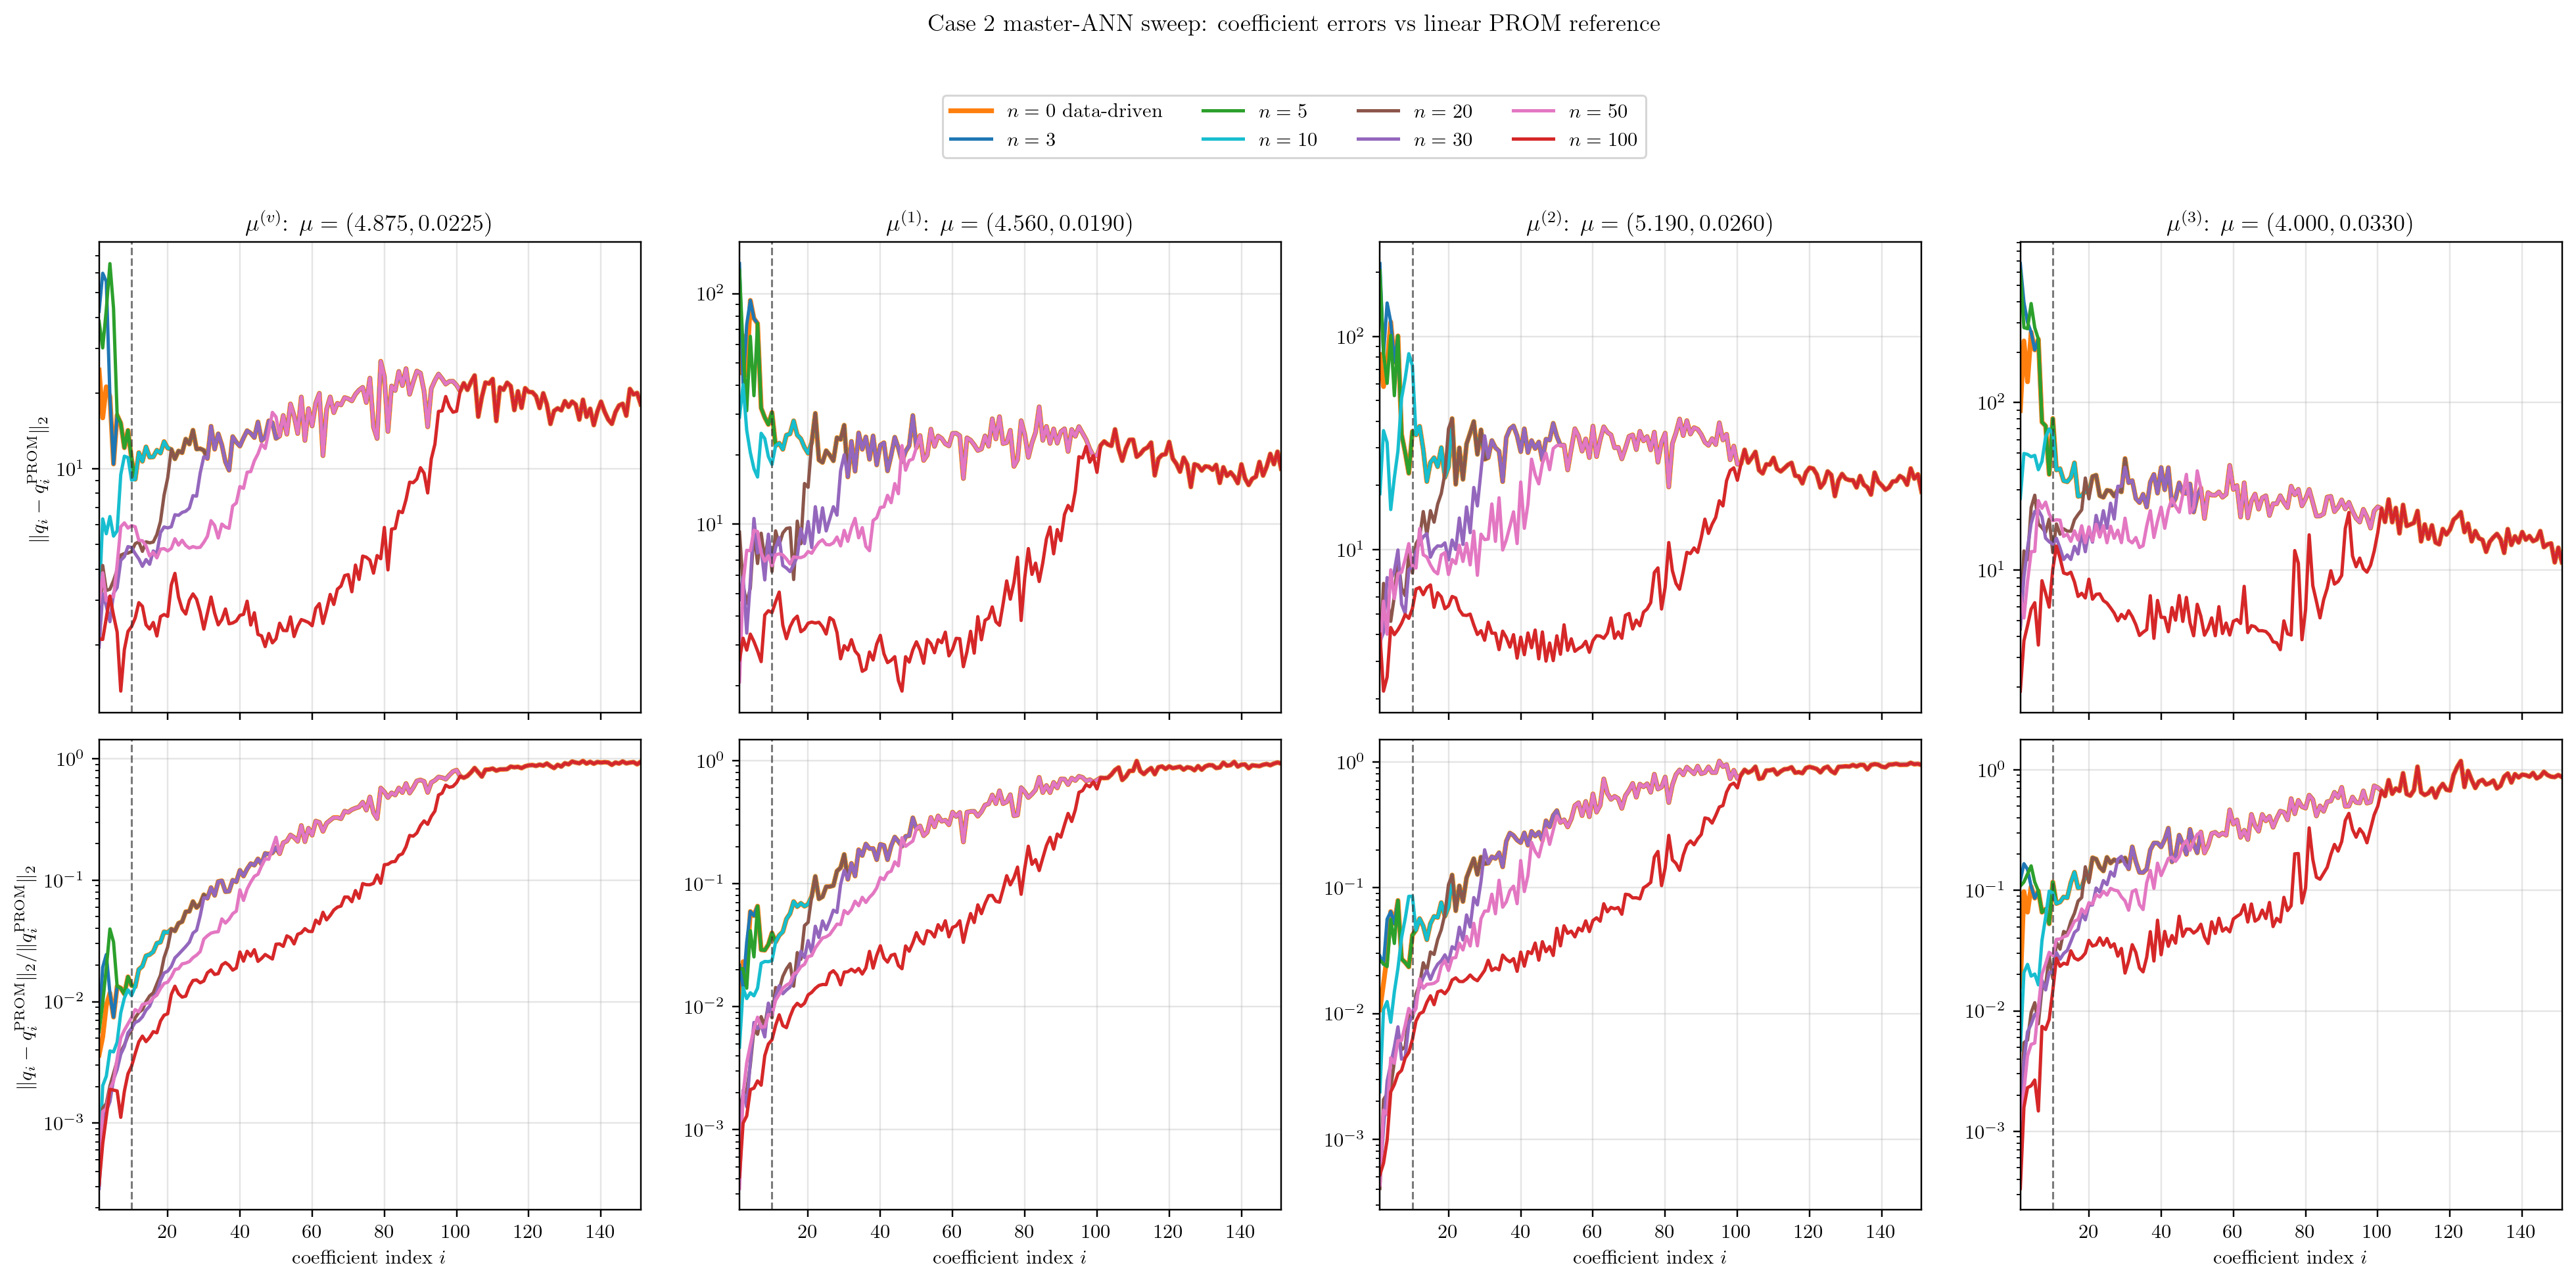
\includegraphics[width=0.98\textwidth]{Figures/prom_only/prom_case2_n_sweep_coeff_abs_rel_all_points.png}
\caption{Case--2 PROM coefficient errors with respect to the linear PROM coefficient trajectories for the same
\(n\)-sweep.  Top: absolute time-trajectory error.  Bottom: relative error.  The dotted vertical line marks
coefficient 10, the primary dimension used in the production Case--2 runs.}
\label{fig:prom-case2-n-sweep-coeff}
\end{figure}

To separate the role of the injected secondary coordinates from the LSPG solve itself, we perturb the secondary
coordinates around the linear PROM values for the fixed \(n=10\) split.  This diagnostic asks how much primary-
coordinate and state error is induced when the secondary tail is no longer exact.

\begin{figure}[H]
\centering
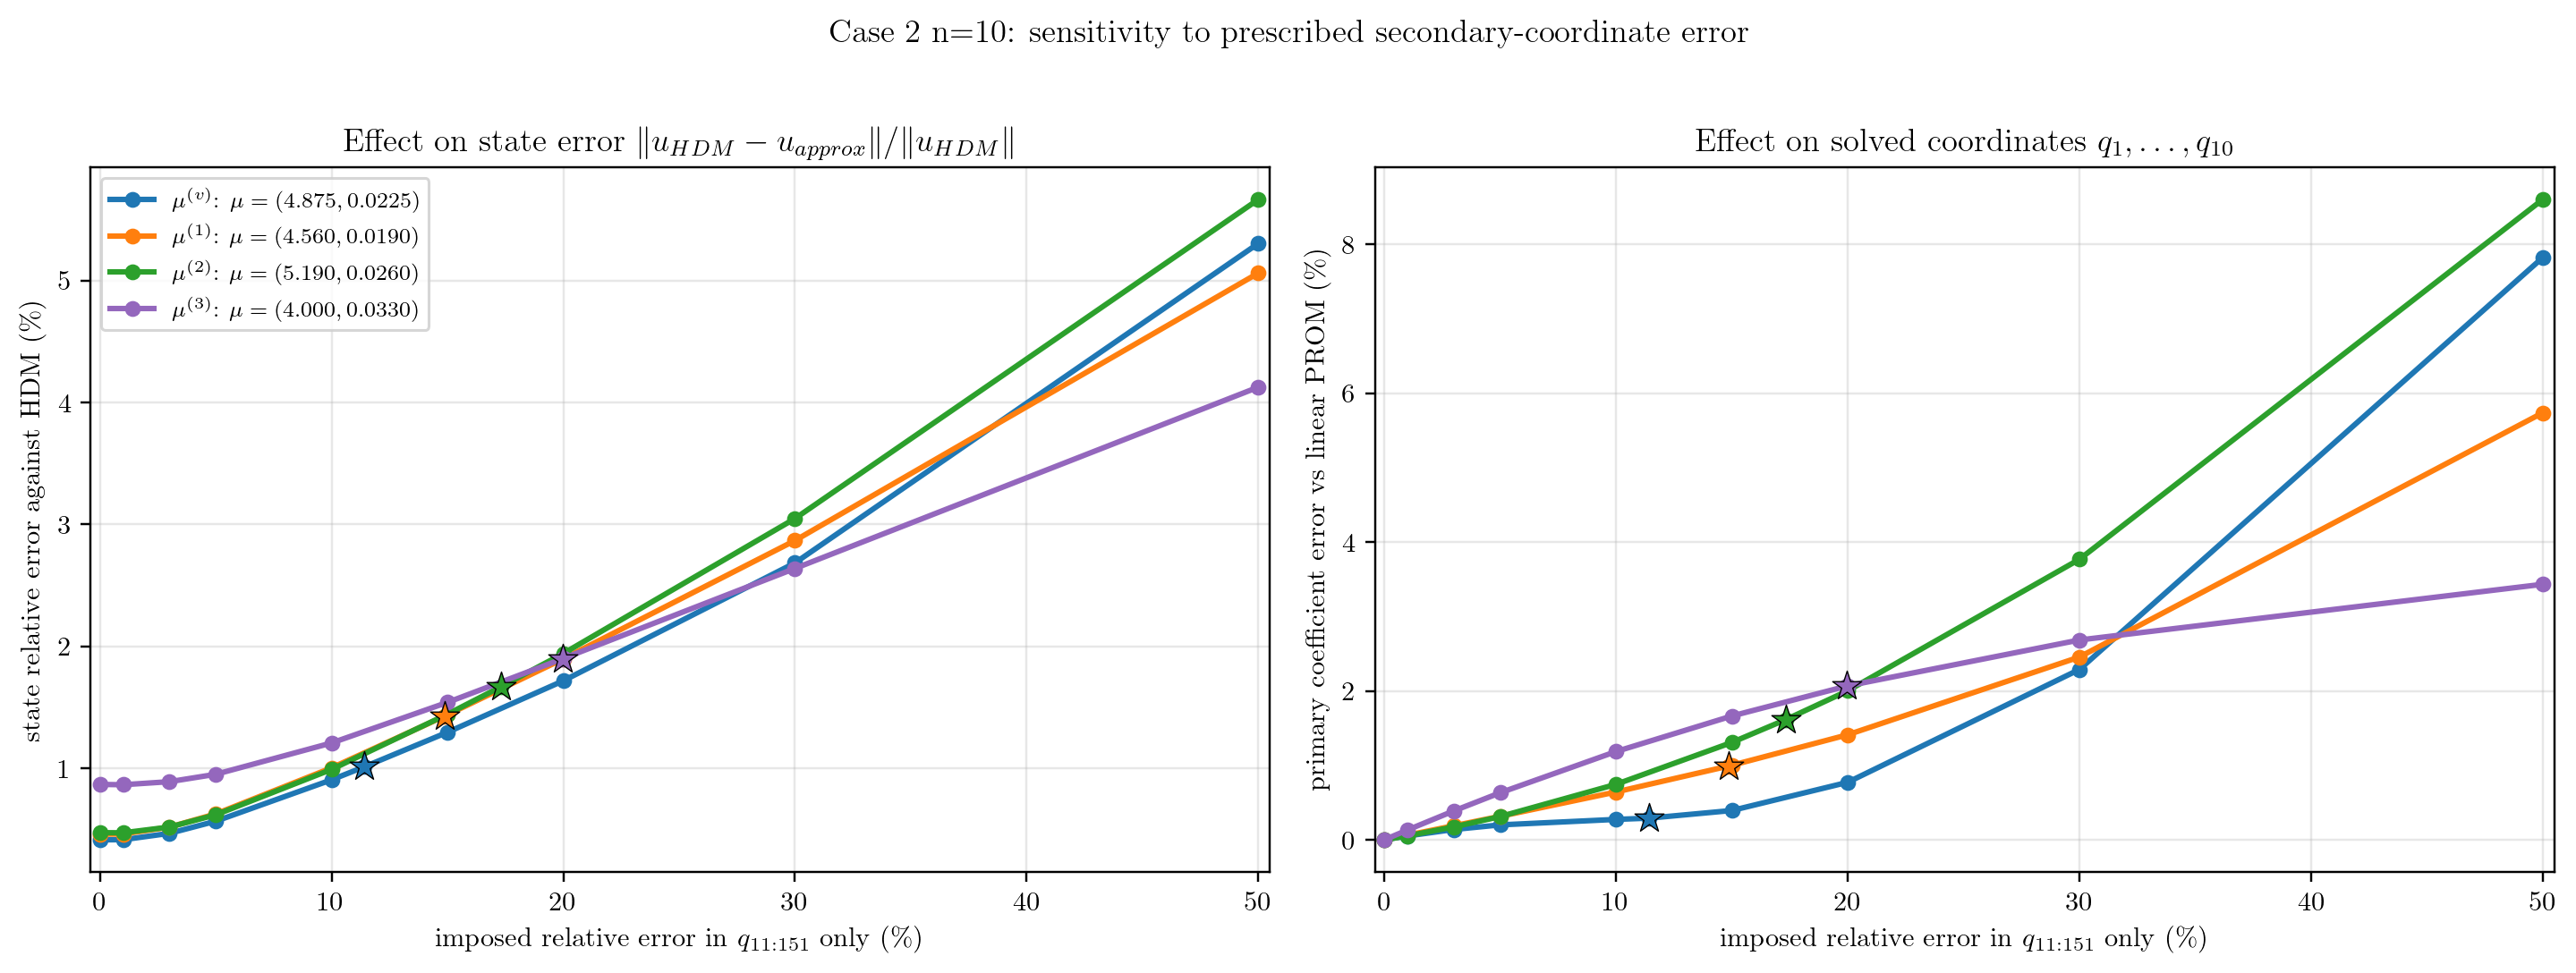
\includegraphics[width=0.95\textwidth]{Figures/prom_only/case2_secondary_sensitivity_state_and_primary_error.png}
\caption{Fixed-split sensitivity of Case--2 PROM with \(n=10\) to prescribed secondary-coordinate error.  Left:
state error against the HDM.  Right: error in the ten solved primary coordinates against the linear PROM.}
\label{fig:prom-case2-secondary-sensitivity}
\end{figure}

The interpretation is that Case 2 is not only a regression problem for the tail.  Tail errors can change the solved
primary coordinates, so the online error reflects both tail-prediction error and residual-solve feedback.

\section{Effect of PROM Data Enrichment}
The enriched campaign tests whether the baseline degradation is primarily an architecture issue or a data-coverage
issue.  The architecture is kept fixed.  The basis \(\V_{151}\), validation points, online evaluation points, and
online PROM formulations are also unchanged.  Only the training coefficient data are expanded from nine PROM
trajectories to 45 PROM trajectories.

\begin{table}[H]
\centering
\caption{Training and validation coefficient errors before and after PROM data enrichment.  The validation set is
kept fixed when available, so the reduction measures generalization improvement rather than a change in evaluation
criterion.}
\label{tab:prom-enrichment-training}
\resizebox{0.9\textwidth}{!}{\begin{tabular}{lrr|rr|rr|rr}
\toprule
& \multicolumn{2}{c|}{Baseline (9)} & \multicolumn{2}{c|}{Early (9+8)} & \multicolumn{2}{c|}{Intermediate (9+18)} & \multicolumn{2}{c}{Enriched (9+36)} \\
Model & train $e_q$ (\%) & val. $e_q$ (\%) & train $e_q$ (\%) & val. $e_q$ (\%) & train $e_q$ (\%) & val. $e_q$ (\%) & train $e_q$ (\%) & val. $e_q$ (\%) \\
\midrule
PROM--ANN Case 1 & 1.130 & 1.251 & 0.742 & 0.825 & 0.512 & 0.557 & 0.360 & 0.374 \\
Master POD--NN--ROM (Case 2 tail source) & 2.601 & 4.391 & 0.983 & 1.625 & 0.580 & 0.814 & 0.435 & 0.555 \\
PROM--ANN Case 3 & 0.405 & 0.482 & 0.311 & 0.347 & 0.289 & 0.324 & 0.230 & 0.268 \\
PROM--POD--AE ($n_z=10$) & 0.106 & 0.127 & 0.087 & 0.098 & 0.084 & 0.095 & 0.054 & 0.074 \\
POD--DL--ROM ($n_z=10$) & 0.810 & 0.935 & 0.348 & 0.362 & 0.246 & 0.273 & 0.142 & 0.158 \\
\bottomrule
\end{tabular}
}
\end{table}

The strongest gain is obtained by the master Case 2/POD--NN map: its validation error decreases from
\(4.391\%\) to \(0.555\%\).  This is the clearest evidence that the previous difficulty was largely caused by the
sparsity of the nine-trajectory parameter training set, not by an intrinsic impossibility of learning the map in this
benchmark.  The POD--DL map also improves strongly, while the already accurate autoencoder still benefits.

\begin{table}[H]
\centering
\caption{Baseline and enriched PROM state errors
\(100\norm{\uvec_{\mathrm{HDM}}-\uvec_{\mathrm{ROM}}}_F/\norm{\uvec_{\mathrm{HDM}}}_F\).  Each mean averages
\(\mub^{(v)},\mub^{(1)},\mub^{(2)}\).  The linear PROM is identical in both blocks because its basis and full
residual formulation are fixed.  The horizontal rule separates residual-evaluating PROMs from the two direct maps.}
\label{tab:prom-enrichment-online}
\resizebox{\textwidth}{!}{\begin{tabular}{lrrrrr|rrrrr}
\toprule
& \multicolumn{5}{c|}{Baseline (9 trajectories)} & \multicolumn{5}{c}{Enriched (9+36 trajectories)} \\
Model & $\mu^{(v)}$ & $\mu^{(1)}$ & $\mu^{(2)}$ & Mean & $\mu^{(3)}$ & $\mu^{(v)}$ & $\mu^{(1)}$ & $\mu^{(2)}$ & Mean & $\mu^{(3)}$ \\
\midrule
Linear PROM & 0.413 & 0.460 & 0.472 & 0.448 & 0.868 & 0.413 & 0.460 & 0.472 & 0.448 & 0.868 \\ 
PROM--ANN Case 1 & 0.409 & 0.520 & 0.683 & 0.537 & 1.584 & 0.411 & 0.459 & 0.469 & 0.446 & 0.868 \\ 
PROM--ANN Case 2 ($n=10$) & 1.013 & 1.427 & 1.670 & 1.370 & 1.898 & 0.435 & 0.477 & 0.496 & 0.469 & 0.872 \\ 
PROM--ANN Case 3 & 0.405 & 0.521 & 0.576 & 0.501 & 1.392 & 0.412 & 0.458 & 0.470 & 0.447 & 0.869 \\ 
PROM--POD--AE ($n_z=10$) & 0.408 & 0.539 & 0.607 & 0.518 & 1.978 & 0.412 & 0.459 & 0.471 & 0.447 & 0.871 \\ 
\midrule
POD--NN--ROM & 1.036 & 1.675 & 1.842 & 1.518 & 3.214 & 0.437 & 0.479 & 0.500 & 0.472 & 0.897 \\ 
POD--DL--ROM ($n_z=10$) & 0.489 & 1.398 & 1.463 & 1.116 & 3.728 & 0.414 & 0.460 & 0.473 & 0.449 & 0.868 \\ 
\bottomrule
\end{tabular}
}
\end{table}

\begin{figure}[H]
\centering

\includegraphics[width=0.98\textwidth]{Figures/prom_only/prom_enrichment_state_error_comparison.png}
\caption{Effect of PROM data enrichment on online state errors.  Left: mean error over the verification and two
off-grid in-domain points.  Right: extrapolatory point.}
\label{fig:prom-enrichment-state}
\end{figure}

\begin{figure}[H]
\centering

\includegraphics[width=0.98\textwidth]{Figures/prom_only/prom_enriched_solution_overlays.png}
\caption{Enriched PROM solution cut-plane comparison against the HDM.  The same seven online models and the same
shared state range as in Fig.~\ref{fig:prom-solution-overlays} are used.  Fainter solid curves are intermediate
times and opaque solid curves are final-time traces; model identity is carried only by colour.}
\label{fig:prom-enriched-solution-overlays}
\end{figure}

After enrichment, all learned models are close to the linear PROM state accuracy at the reported points.  The most
important qualitative change is that the non-intrusive maps no longer behave as outliers: the enriched POD--NN--ROM
and POD--DL--ROM have state errors comparable to the intrusive learned PROMs.  For the extrapolatory point, the
enriched errors also collapse near the fixed linear PROM level, indicating that the exterior LHS samples provide
useful information in the expanded parameter region.

\begin{table}[H]
\centering
\caption{Baseline and enriched PROM coefficient errors against the corresponding fixed \(n_{\mathrm{tot}}=151\)
linear PROM coefficient trajectory.  Values are relative Frobenius percentages over all coefficients and time
steps.  The horizontal rule separates residual-evaluating PROMs from the two direct maps.}
\label{tab:prom-enrichment-coeff}
\resizebox{0.9\textwidth}{!}{\begin{tabular}{lrrrrr|rrrrr}
\toprule
& \multicolumn{5}{c|}{Baseline (9 trajectories)} & \multicolumn{5}{c}{Enriched (9+36 trajectories)} \\
Model & $\mu^{(v)}$ & $\mu^{(1)}$ & $\mu^{(2)}$ & Mean & $\mu^{(3)}$ & $\mu^{(v)}$ & $\mu^{(1)}$ & $\mu^{(2)}$ & Mean & $\mu^{(3)}$ \\
\midrule
Linear PROM & 0.000 & 0.000 & 0.000 & 0.000 & 0.000 & 0.000 & 0.000 & 0.000 & 0.000 & 0.000 \\ 
PROM--ANN Case 1 & 0.295 & 0.593 & 1.297 & 0.729 & 2.923 & 0.066 & 0.057 & 0.089 & 0.070 & 0.178 \\ 
PROM--ANN Case 2 ($n=10$) & 2.440 & 3.361 & 3.906 & 3.236 & 4.257 & 0.377 & 0.357 & 0.433 & 0.389 & 0.583 \\ 
PROM--ANN Case 3 & 0.164 & 0.856 & 0.788 & 0.603 & 2.396 & 0.039 & 0.038 & 0.055 & 0.044 & 0.117 \\ 
PROM--POD--AE ($n_z=10$) & 0.140 & 0.773 & 0.929 & 0.614 & 4.394 & 0.041 & 0.041 & 0.059 & 0.047 & 0.151 \\ 
\midrule
POD--NN--ROM & 2.499 & 3.924 & 4.249 & 3.557 & 7.444 & 0.385 & 0.362 & 0.446 & 0.398 & 0.805 \\ 
POD--DL--ROM ($n_z=10$) & 0.814 & 3.129 & 3.225 & 2.389 & 8.639 & 0.108 & 0.099 & 0.130 & 0.112 & 0.240 \\ 
\bottomrule
\end{tabular}
}
\end{table}

\begin{figure}[H]
\centering

\includegraphics[width=0.98\textwidth]{Figures/prom_only/prom_enrichment_coeff_error_comparison.png}
\caption{Effect of PROM data enrichment on online coefficient errors.  The coefficient metric is stricter than the
state metric because it measures the entire \(151\)-coordinate trajectory against the linear PROM teacher.}
\label{fig:prom-enrichment-coeff}
\end{figure}

\begin{figure}[H]
\centering

\includegraphics[width=0.98\textwidth]{Figures/prom_only/prom_enriched_coeff_abs_rel_errors.png}
\caption{Enriched PROM online coefficient errors against the enriched linear-PROM reference.  The plotted set is
identical to Fig.~\ref{fig:prom-coeff-rel-errors}: Case 1, Case 2 with \(n=10\), Case 3, PROM--POD--AE,
POD--NN--ROM, and POD--DL--ROM.  Shared ordinate ranges permit a direct baseline--enriched comparison.}
\label{fig:prom-enriched-coeff-errors}
\end{figure}

The coefficient table confirms the state-error interpretation.  The baseline POD--NN--ROM has an in-domain mean
coefficient error of \(3.557\%\) and \(7.444\%\) at the extrapolatory point.  After enrichment these decrease to
\(0.398\%\) and \(0.805\%\), respectively.  Case 2 with \(n=10\) improves similarly because it uses the same master
map for the injected tail.

\begin{figure}[H]
\centering

\includegraphics[width=0.98\textwidth]{Figures/prom_only/prom_enriched_coeff_abs_heatmaps.png}
\caption{Enriched PROM time-by-coefficient absolute errors against the enriched linear PROM.  Rows include the four
intrusive learned PROMs followed by POD--NN--ROM and POD--DL--ROM.  The colour range and the coefficient-10
separator are identical to the baseline PROM heatmap in Fig.~\ref{fig:prom-coeff-abs-heatmaps}.}
\label{fig:prom-enriched-coeff-abs-heatmaps}
\end{figure}

\begin{figure}[H]
\centering

\includegraphics[width=0.98\textwidth]{Figures/prom_only/prom_enriched_coeff_rel_heatmaps.png}
\caption{Enriched PROM time-by-coefficient relative errors.  The shared \(0\)--\(20\%\) colour range exposes the
low-error structure recovered by enrichment while clipping only larger values.}
\label{fig:prom-enriched-coeff-rel-heatmaps}
\end{figure}

\begin{figure}[H]
\centering

\includegraphics[width=0.98\textwidth]{Figures/prom_only/prom_enrichment_case2_coeff_rel_errors.png}
\caption{Case--2 per-coefficient relative error before and after PROM data enrichment for \(n=10\).  The vertical
line marks the separation between the ten residual-solved primary coordinates and the ANN-injected secondary tail.
The linear PROM coefficient trajectory is the reference.}
\label{fig:prom-enrichment-case2-coeff}
\end{figure}

Figure~\ref{fig:prom-enrichment-case2-coeff} shows the mechanism relevant to the intrusive closure itself.  With
only nine trajectories, the ANN-injected tail has relative errors close to order one even when the global state error
is moderate.  The enriched training set reduces those tail errors over most coefficients, while the LSPG solve
continues to recover the leading ten coordinates.  This is why the Case--2 residual is far less feedback-sensitive
after enrichment.

\section{Baseline HPROM Results}
The HPROM campaign uses the same MLSPG-sensitive basis and the same baseline nine-trajectory training set, but
replaces the full residual evaluations by empirical cubature.  The cubature rules are built from 2\% of the
available parameter--time residual snapshots using a global parameter--time stratified selection and direct dense
SVD before ECM.  The linear HPROM uses its own ECM rule for the \(151\)-coordinate linear residual problem.  Each
learned intrusive family uses a separate rule matched to its online residual and unknown dimension.  This avoids the
earlier ambiguity of applying an unrelated linear rule to a nonlinear learned residual.

\begin{table}[H]
\centering
\caption{Baseline HPROM cubature setup.  The learned \(n=10\) rows cover Case 1, Case 2 with \(n=10\), Case 3, and
PROM--POD--AE; Case 2 with \(n=20\) uses the larger \(n=20\) rule.}
\label{tab:hprom-ecm-setup}
\resizebox{0.9\textwidth}{!}{\begin{tabular}{lrrl}
\toprule
Family & Snapshot pct. & $N_{\rm ECM}$ & SVD / sampling rule \\
\midrule
Linear HPROM & 2.0 & 5975 & direct dense SVD, global parameter--time stratified \\
Learned HPROM, $n=10$ & 2.0 & 901 & direct dense SVD, global parameter--time stratified \\
Learned HPROM, $n=20$ & 2.0 & 1801 & direct dense SVD, global parameter--time stratified \\
\bottomrule
\end{tabular}
}
\end{table}

\begin{table}[H]
\centering
\caption{Baseline HPROM Stage--3 selected networks.  The full-coordinate master map is shared by POD--NN-ROM and
Case 2; the online Case 2 solver trims this \(q_{151}\) prediction and solves the first \(n\) coordinates.  Errors
are relative Frobenius percentages in coefficient space.}
\label{tab:hprom-training}
\resizebox{\textwidth}{!}{\begin{tabular}{llrrrr}
\toprule
Model & Map / network & Act. & Train $e_q$ (\%) & Val. $e_q$ (\%) & Params \\
\midrule
HPROM--ANN Case 1 & $\q_p\mapsto\q_s$; $10\to256\to512\to512\to256\to141$ & SiLU & 0.992 & 1.101 & 564,621 \\
Master POD--NN--ROM (Case 2 tail source) & $(\mu_1,\mu_2,t)\mapsto\q_{151}$; $3\to256\to512\to512\to256\to151$ & SiLU & 0.975 & 1.124 & 565,399 \\
HPROM--ANN Case 3 & $(\q_p,\mu_1,\mu_2,t)\mapsto\q_s$; $13\to256\to512\to512\to256\to141$ & SiLU & 0.491 & 0.577 & 565,389 \\
HPROM-POD-AE & z-score AE; $151\to512\to256\to128\to10\to128\to256\to512\to151$ & GELU & 0.098 & 0.119 & 486,817 \\
POD--DL--ROM & z-score latent dynamics; $3\to256\to512\to512\to256\to10\to151$ & SiLU & 0.624 & 0.744 & 952,747 \\
\bottomrule
\end{tabular}
}
\end{table}

Table~\ref{tab:hprom-online} reports the HPROM state errors.  The linear HPROM is the sampled-residual analogue of
the linear PROM reference.  Its in-domain mean error is \(0.448\%\), compared with \(0.868\%\) at the extrapolatory
point.  Case 1, Case 3, and PROM--POD--AE remain close to this reference in the three in-domain tests.  Case 2 is
more sensitive: with \(n=10\), the off-grid and extrapolatory errors increase substantially; increasing the solved
primary dimension to \(n=20\) reduces that error, but does not make Case 2 as robust as Case 1, Case 3, or
PROM--POD--AE.

\begin{table}[H]
\centering
\caption{Baseline HPROM online errors
\(100\norm{\uvec_{\mathrm{HDM}}-\uvec_{\mathrm{ROM}}}_F/\norm{\uvec_{\mathrm{HDM}}}_F\).  The mean column averages
\(\mub^{(v)},\mub^{(1)},\mub^{(2)}\).  The horizontal rule separates residual-evaluating HPROMs from the
two direct non-intrusive maps, which do not perform an online sampled-residual solve.  The corresponding ECM
cardinalities are reported separately in Table~\ref{tab:hprom-ecm-setup}.}
\label{tab:hprom-online}
\resizebox{\textwidth}{!}{\begin{tabular}{lrrrrrr}
\toprule
Model & $\mu^{(v)}$ & $\mu^{(1)}$ & $\mu^{(2)}$ & Mean & $\mu^{(3)}$ & Mean time (s) \\
\midrule
Linear HPROM & 0.413 & 0.460 & 0.472 & 0.448 & 0.868 & 99.03 \\
HPROM--ANN Case 1 & 0.423 & 0.575 & 0.702 & 0.567 & 1.547 & 18.57 \\
HPROM--ANN Case 2 ($n=10$) & 0.512 & 4.516 & 2.895 & 2.641 & 13.098 & 5.81 \\
HPROM--ANN Case 2 ($n=20$) & 0.510 & 1.484 & 1.994 & 1.329 & 3.504 & 8.16 \\
HPROM--ANN Case 3 & 0.415 & 0.514 & 0.592 & 0.507 & 1.416 & 18.90 \\
HPROM-POD-AE ($n_z=10$) & 0.442 & 0.627 & 0.658 & 0.575 & 1.787 & 17.52 \\
\midrule
POD--NN--ROM & 0.508 & 1.834 & 2.479 & 1.607 & 7.401 & 0.06 \\
POD--DL--ROM ($n_z=10$) & 0.451 & 1.483 & 1.498 & 1.144 & 4.753 & 0.02 \\
\bottomrule
\end{tabular}
}
\end{table}

\begin{figure}[H]
\centering
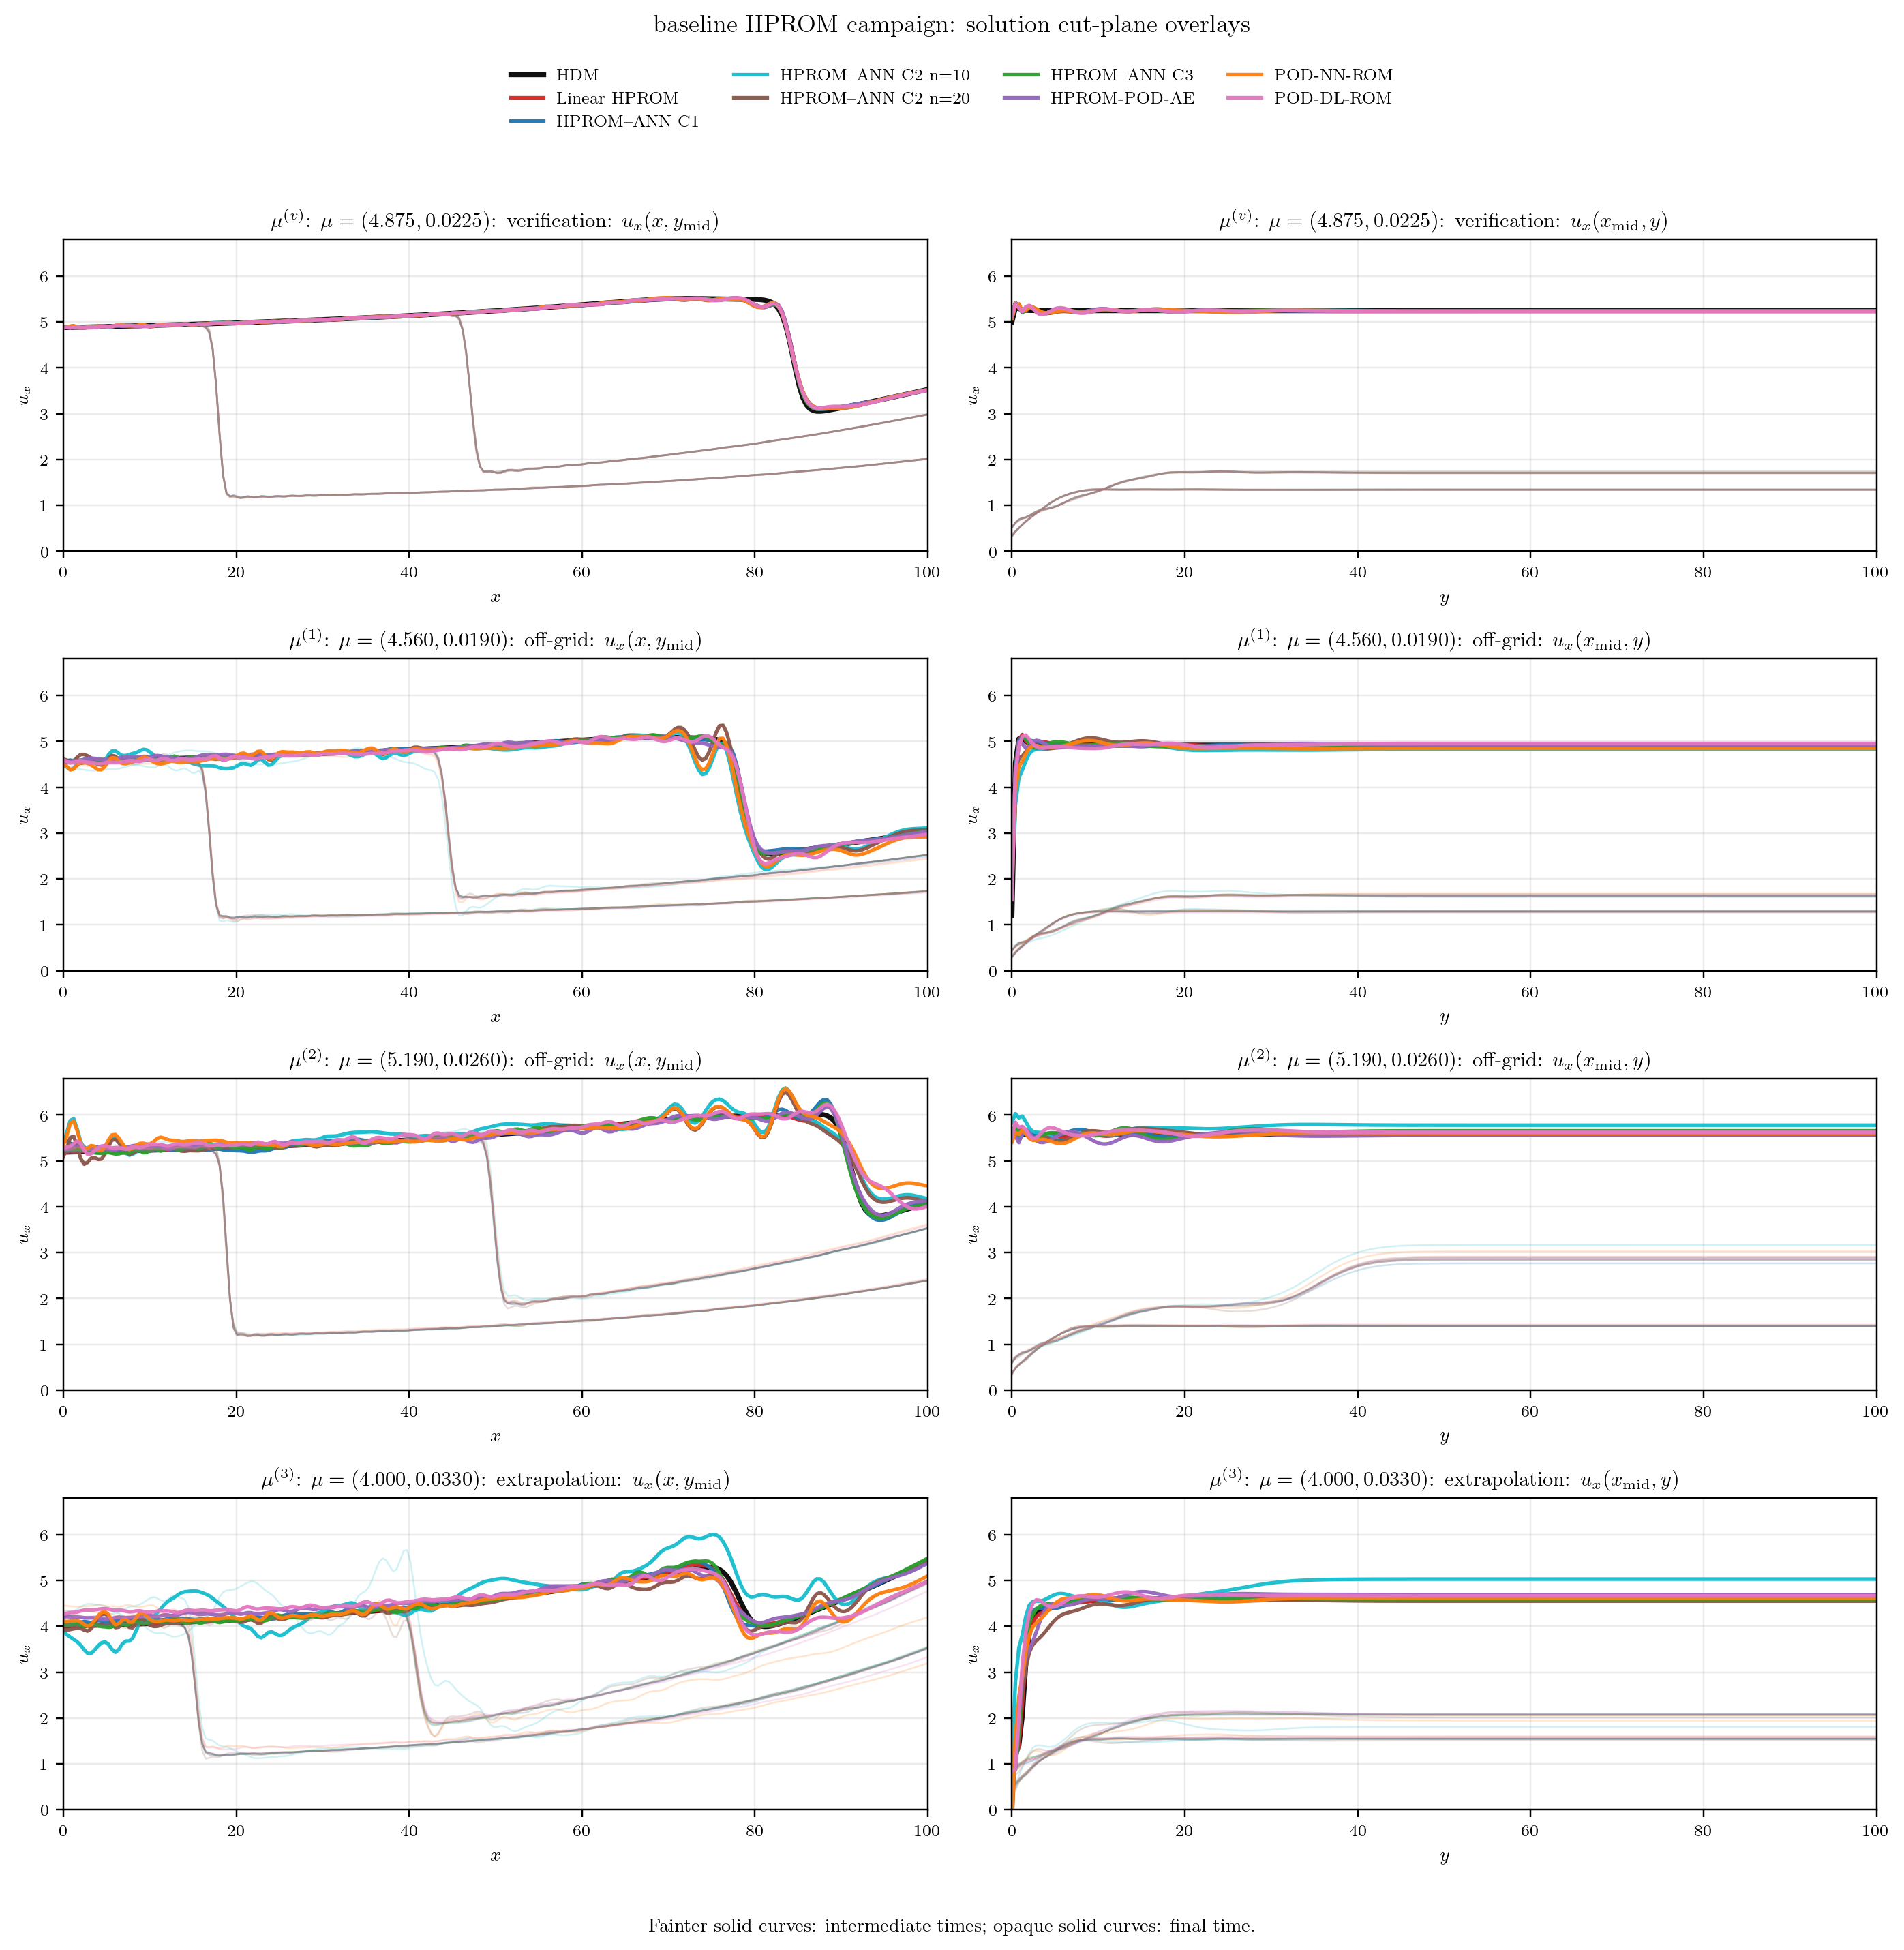
\includegraphics[width=0.98\textwidth]{Figures/hprom_only/hprom_baseline_solution_overlays.png}
\caption{Baseline HPROM solution cut-plane comparison against the HDM at the four evaluation points.  The layout,
solid-curve time-opacity convention, state range, and method colors are identical to those in
Fig.~\ref{fig:prom-solution-overlays}.  The linear HPROM curves are reconstructed from their saved coefficient
trajectories; the nonlinear HPROM curves use the saved online state snapshots.}
\label{fig:hprom-solution-overlays}
\end{figure}

The overlay in Fig.~\ref{fig:hprom-solution-overlays} shows that the large Case 2 errors are not a table artifact.
For \(n=10\), the injected tail perturbs the sampled residual enough to produce visible oscillations at the
off-grid and extrapolatory points.  The \(n=20\) version damps much of this behavior because more of the leading
coefficient subspace is recovered by the online solve.

\begin{table}[H]
\centering
\caption{Baseline HPROM online coefficient error against the linear HPROM with \(n_{\mathrm{tot}}=151\).  Values
are relative Frobenius percentages over all 151 coefficients and all time steps.  The final two rows are the direct
non-intrusive maps and are separated from the residual-evaluating HPROMs by a horizontal rule.}
\label{tab:hprom-online-coeff}
\resizebox{0.9\textwidth}{!}{\begin{tabular}{lrrrrr}
\toprule
Model & $\mu^{(v)}$ & $\mu^{(1)}$ & $\mu^{(2)}$ & Mean & $\mu^{(3)}$ \\
\midrule
Linear HPROM & 0.000 & 0.000 & 0.000 & 0.000 & 0.000 \\
HPROM--ANN Case 1 & 0.245 & 0.593 & 1.250 & 0.696 & 2.899 \\
HPROM--ANN Case 2 ($n=10$) & 0.924 & 4.375 & 4.814 & 3.371 & 9.996 \\
HPROM--ANN Case 2 ($n=20$) & 0.921 & 3.105 & 4.377 & 2.801 & 6.981 \\
HPROM--ANN Case 3 & 0.242 & 0.819 & 0.775 & 0.612 & 2.296 \\
HPROM-POD-AE ($n_z=10$) & 0.273 & 0.839 & 1.122 & 0.745 & 4.004 \\
\midrule
POD--NN--ROM & 0.929 & 4.192 & 5.642 & 3.588 & 17.433 \\
POD--DL--ROM ($n_z=10$) & 0.616 & 3.334 & 3.291 & 2.413 & 11.101 \\
\bottomrule
\end{tabular}
}
\end{table}

\begin{figure}[H]
\centering
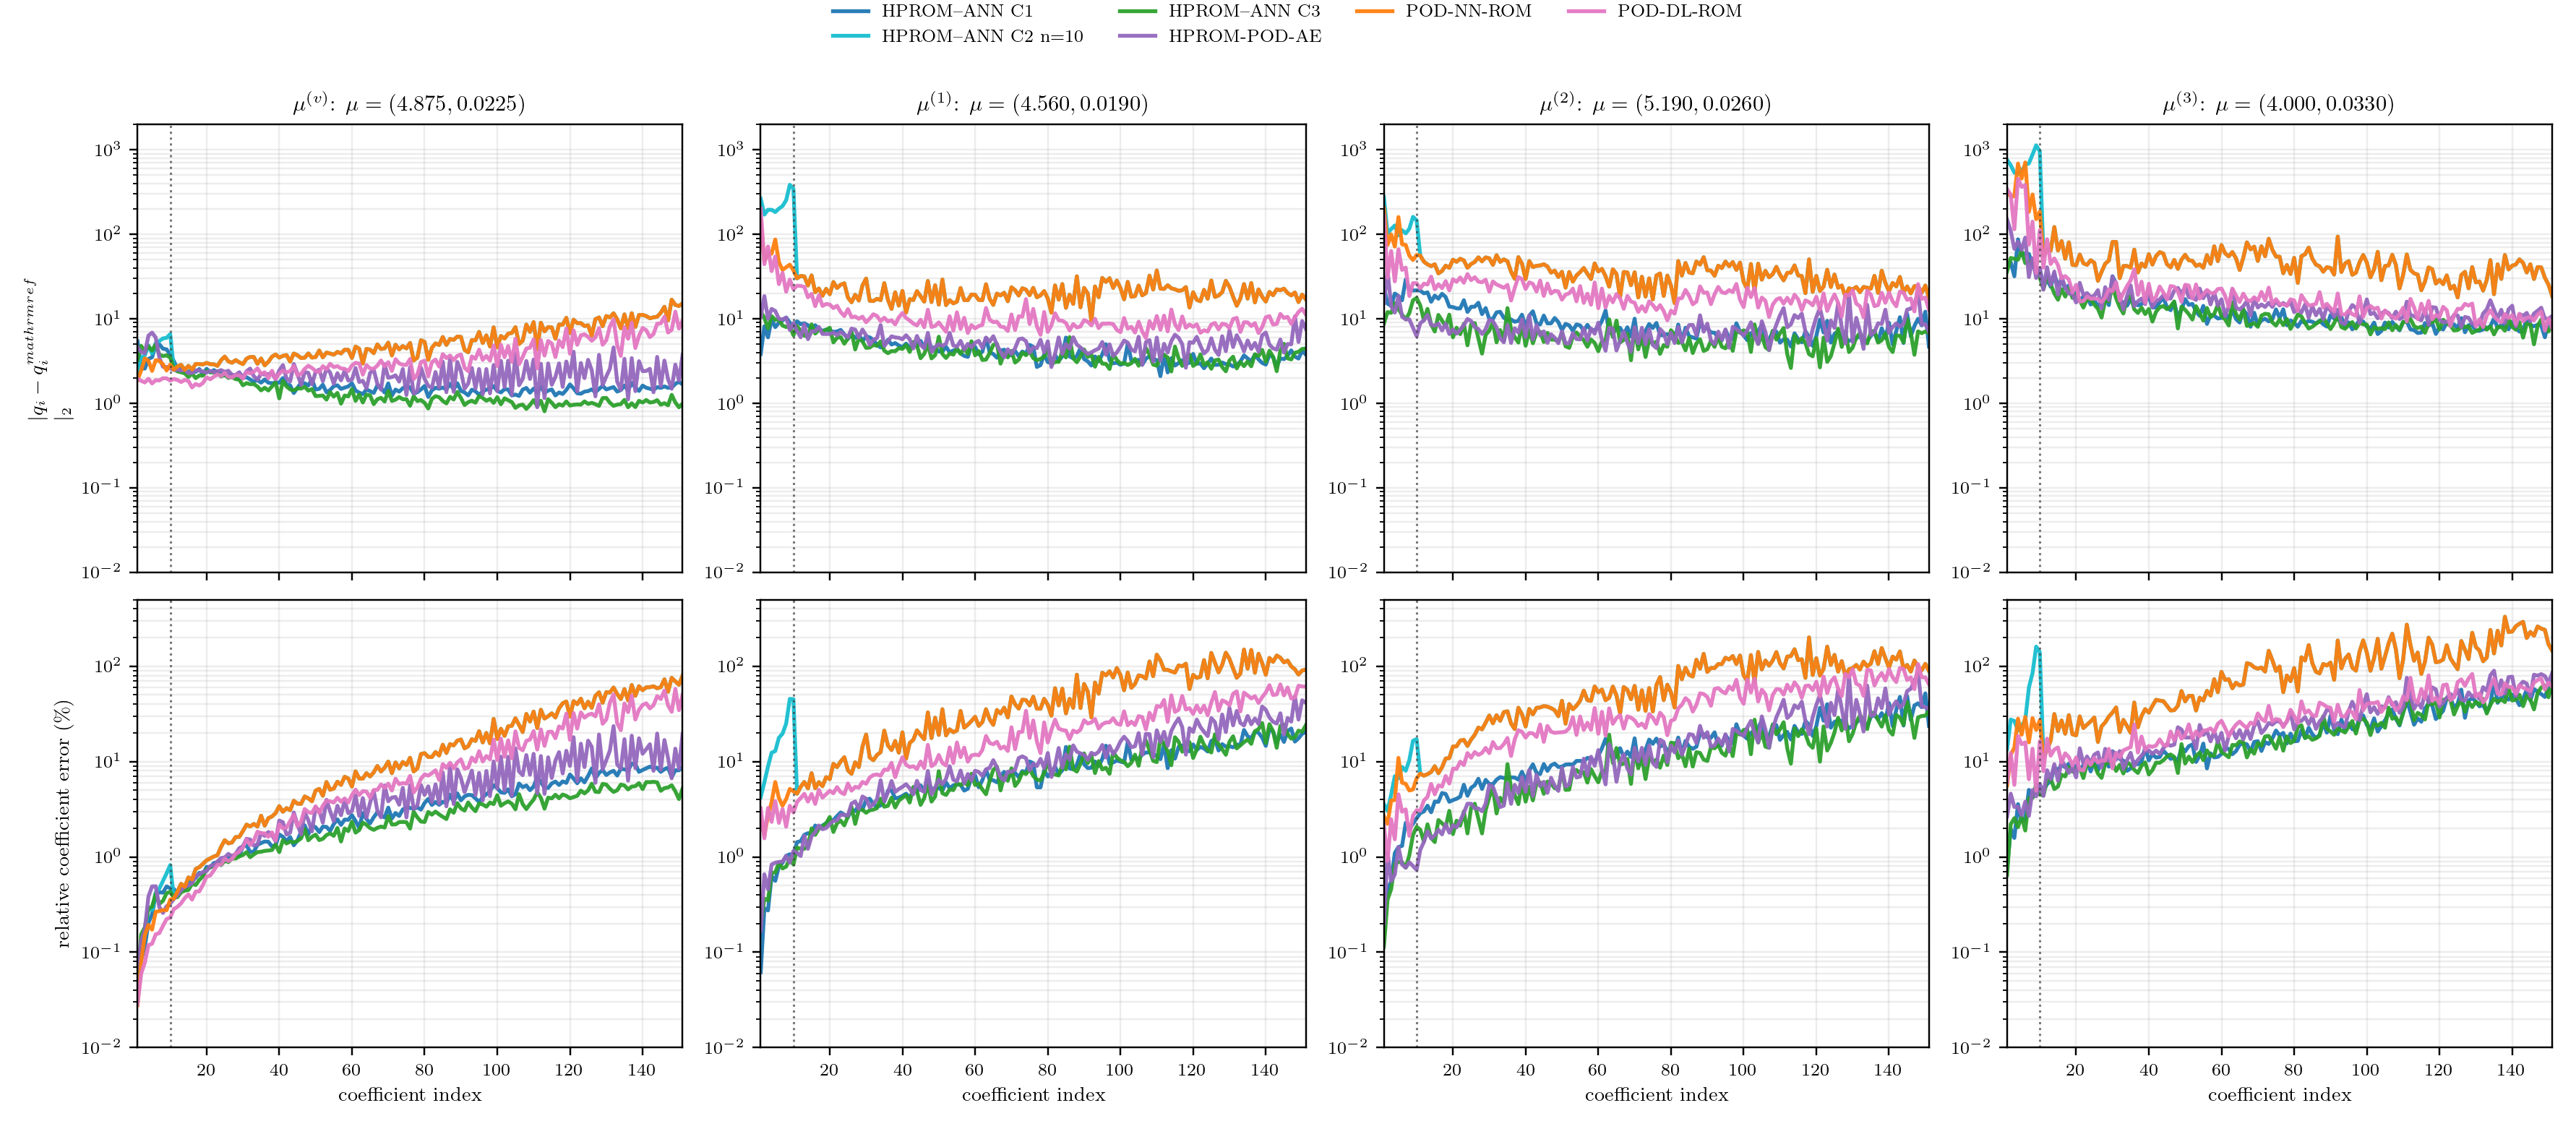
\includegraphics[width=0.98\textwidth]{Figures/hprom_only/hprom_baseline_coeff_abs_rel_errors.png}
\caption{Baseline HPROM online coefficient errors against the \(n_{\mathrm{tot}}=151\) linear HPROM trajectory.
Top: absolute trajectory error. Bottom: relative trajectory error.  Intrusive closures and the two direct
non-intrusive maps are all included from their saved online outputs.  The PROM and HPROM coefficient figures use the
same fixed ordinate ranges, and the vertical line marks coefficient 10.  The linear HPROM itself is the reference
and is not plotted.}
\label{fig:hprom-coeff-rel-errors}
\end{figure}

The HPROM coefficient diagnostics mirror the PROM-level mechanism.  The high-index tail is the difficult part of
the learned map, and Case 2 is the most exposed to this difficulty because its tail is injected directly into the
online residual.  The \(n=20\) Case 2 run improves both state and coefficient errors relative to \(n=10\), but the
remaining tail error is still large for the extrapolatory point.  Case 3 is the most accurate learned HPROM in
coefficient space because it combines residual-solved primary coordinates with explicit \((\mu_1,\mu_2,t)\)
information in the closure.

\begin{figure}[H]
\centering
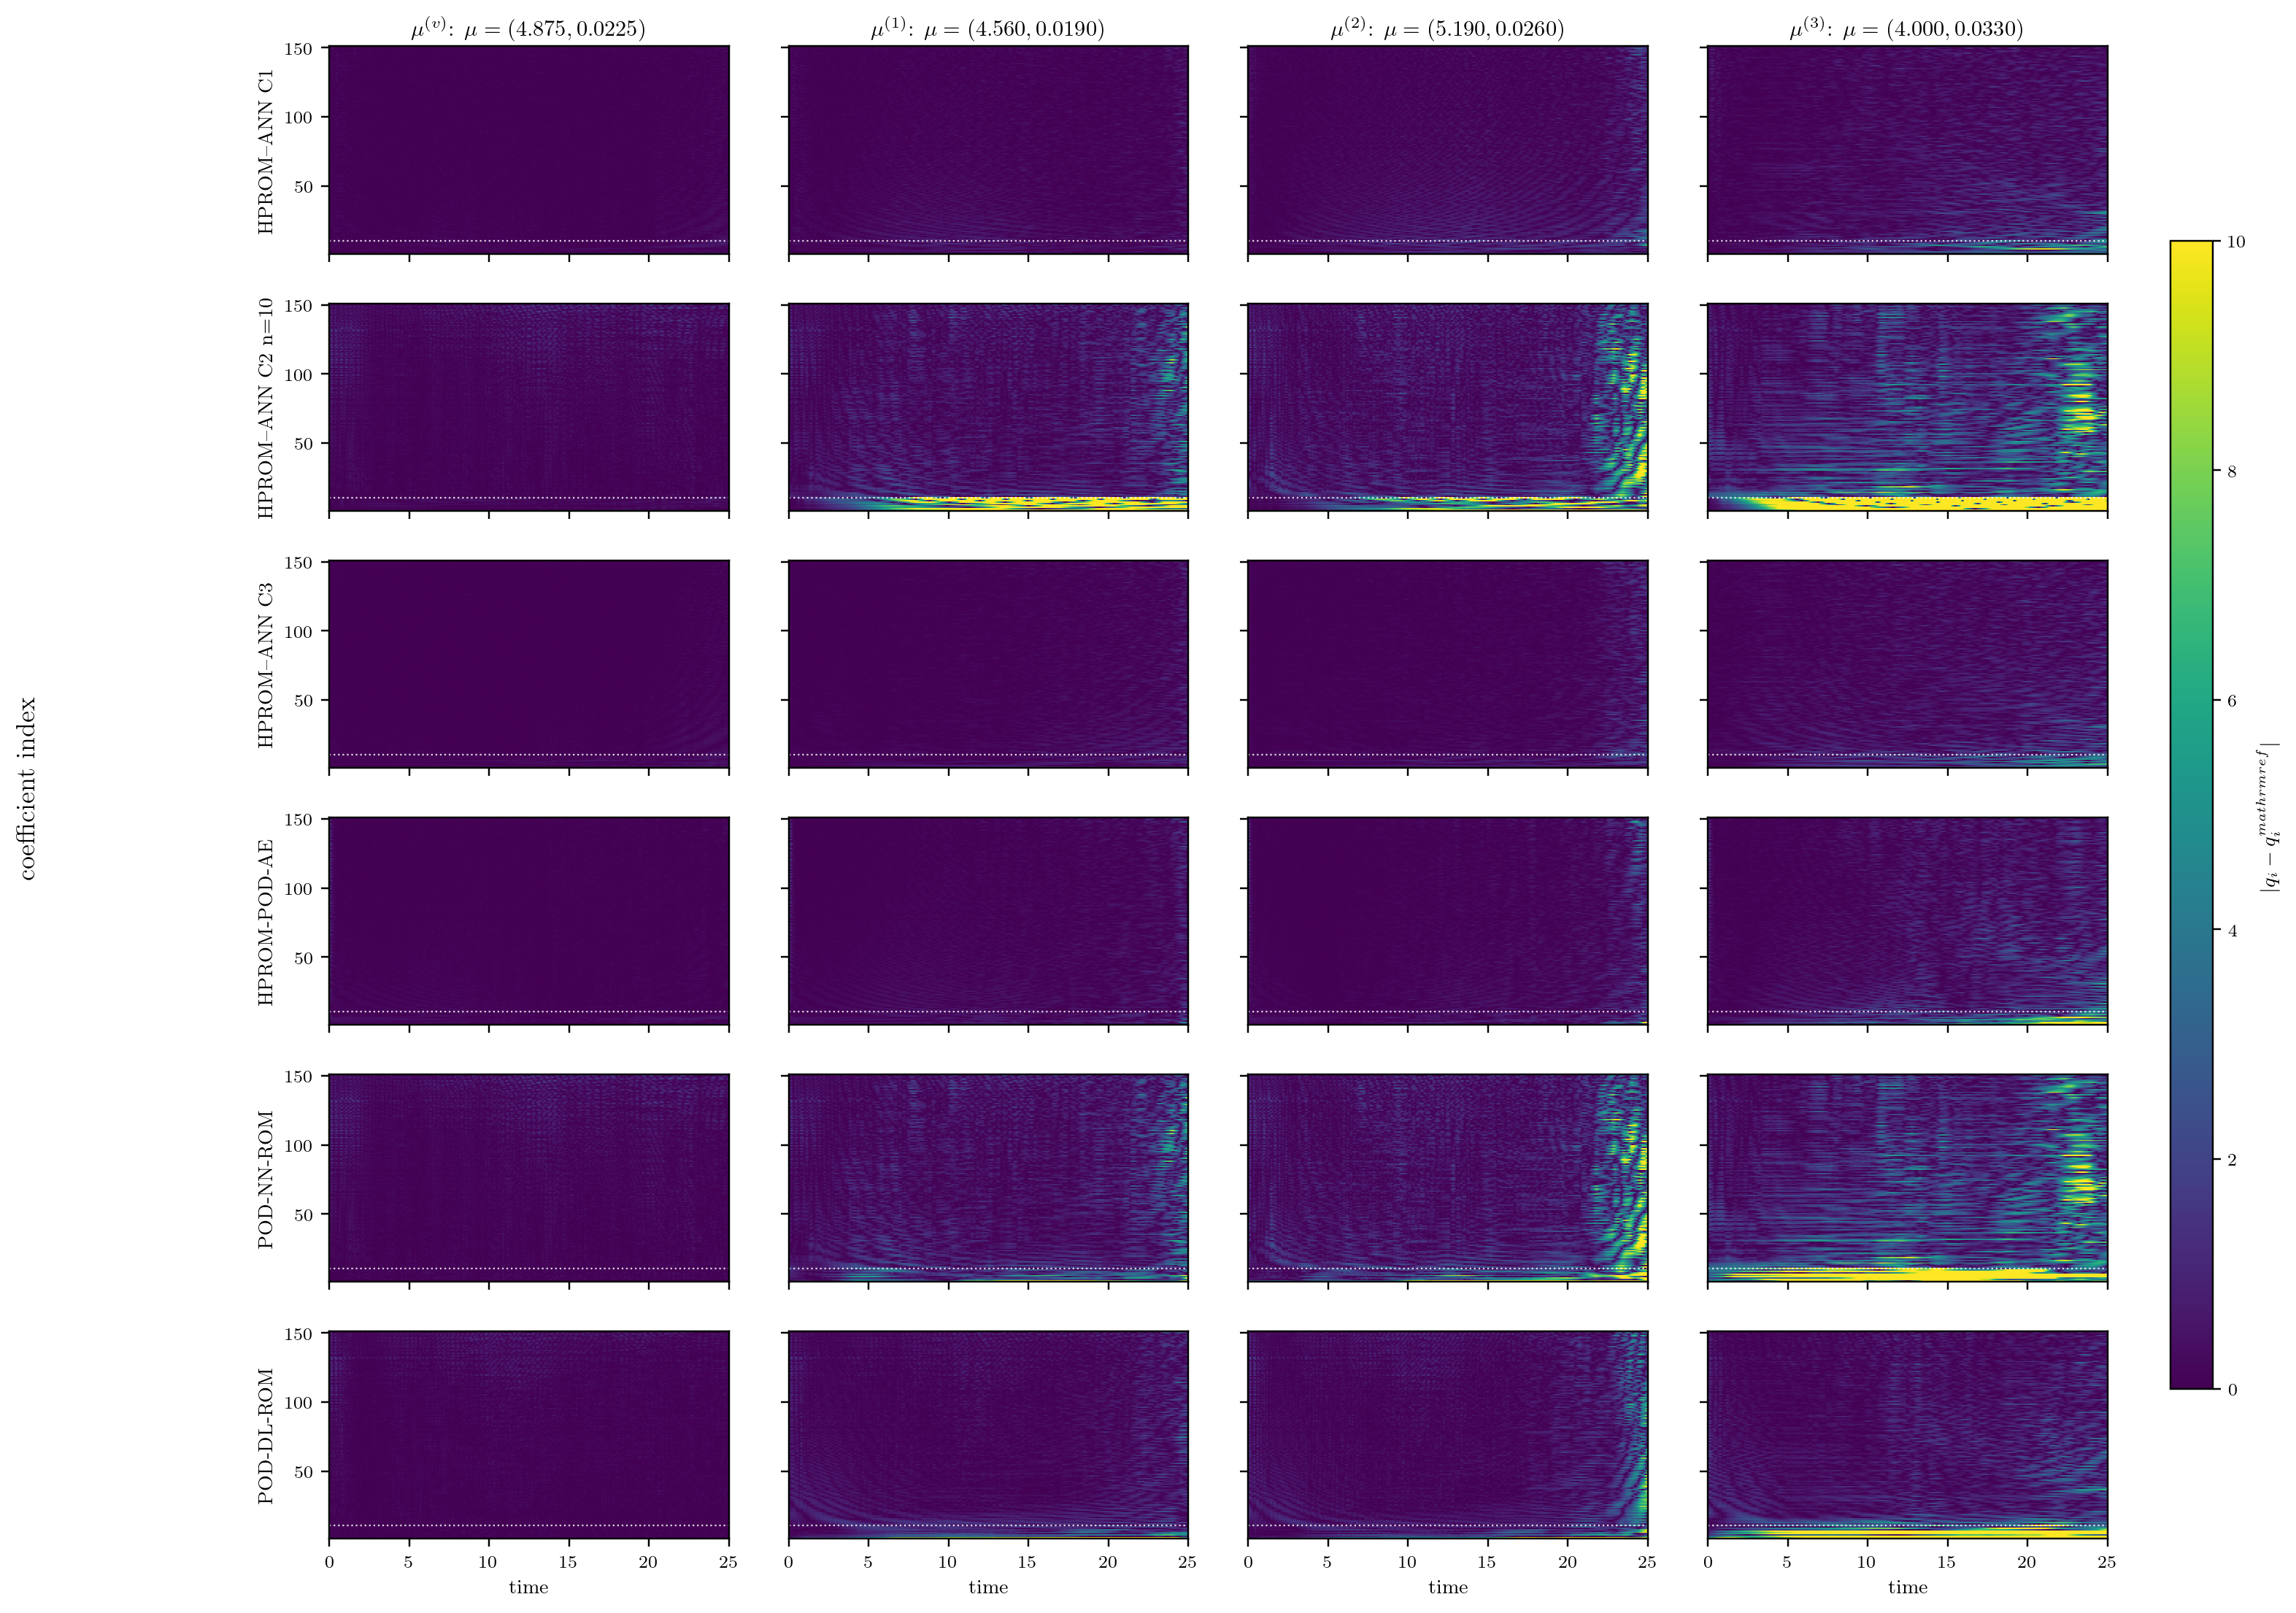
\includegraphics[width=0.98\textwidth]{Figures/hprom_only/hprom_baseline_coeff_abs_heatmaps.png}
\caption{Baseline HPROM time-by-coefficient absolute errors against the linear HPROM.  The row/column ordering,
the primary-coordinate separator, and the absolute colour range are identical to those of
Fig.~\ref{fig:prom-coeff-abs-heatmaps}.}
\label{fig:hprom-coeff-abs-heatmaps}
\end{figure}

\begin{figure}[H]
\centering
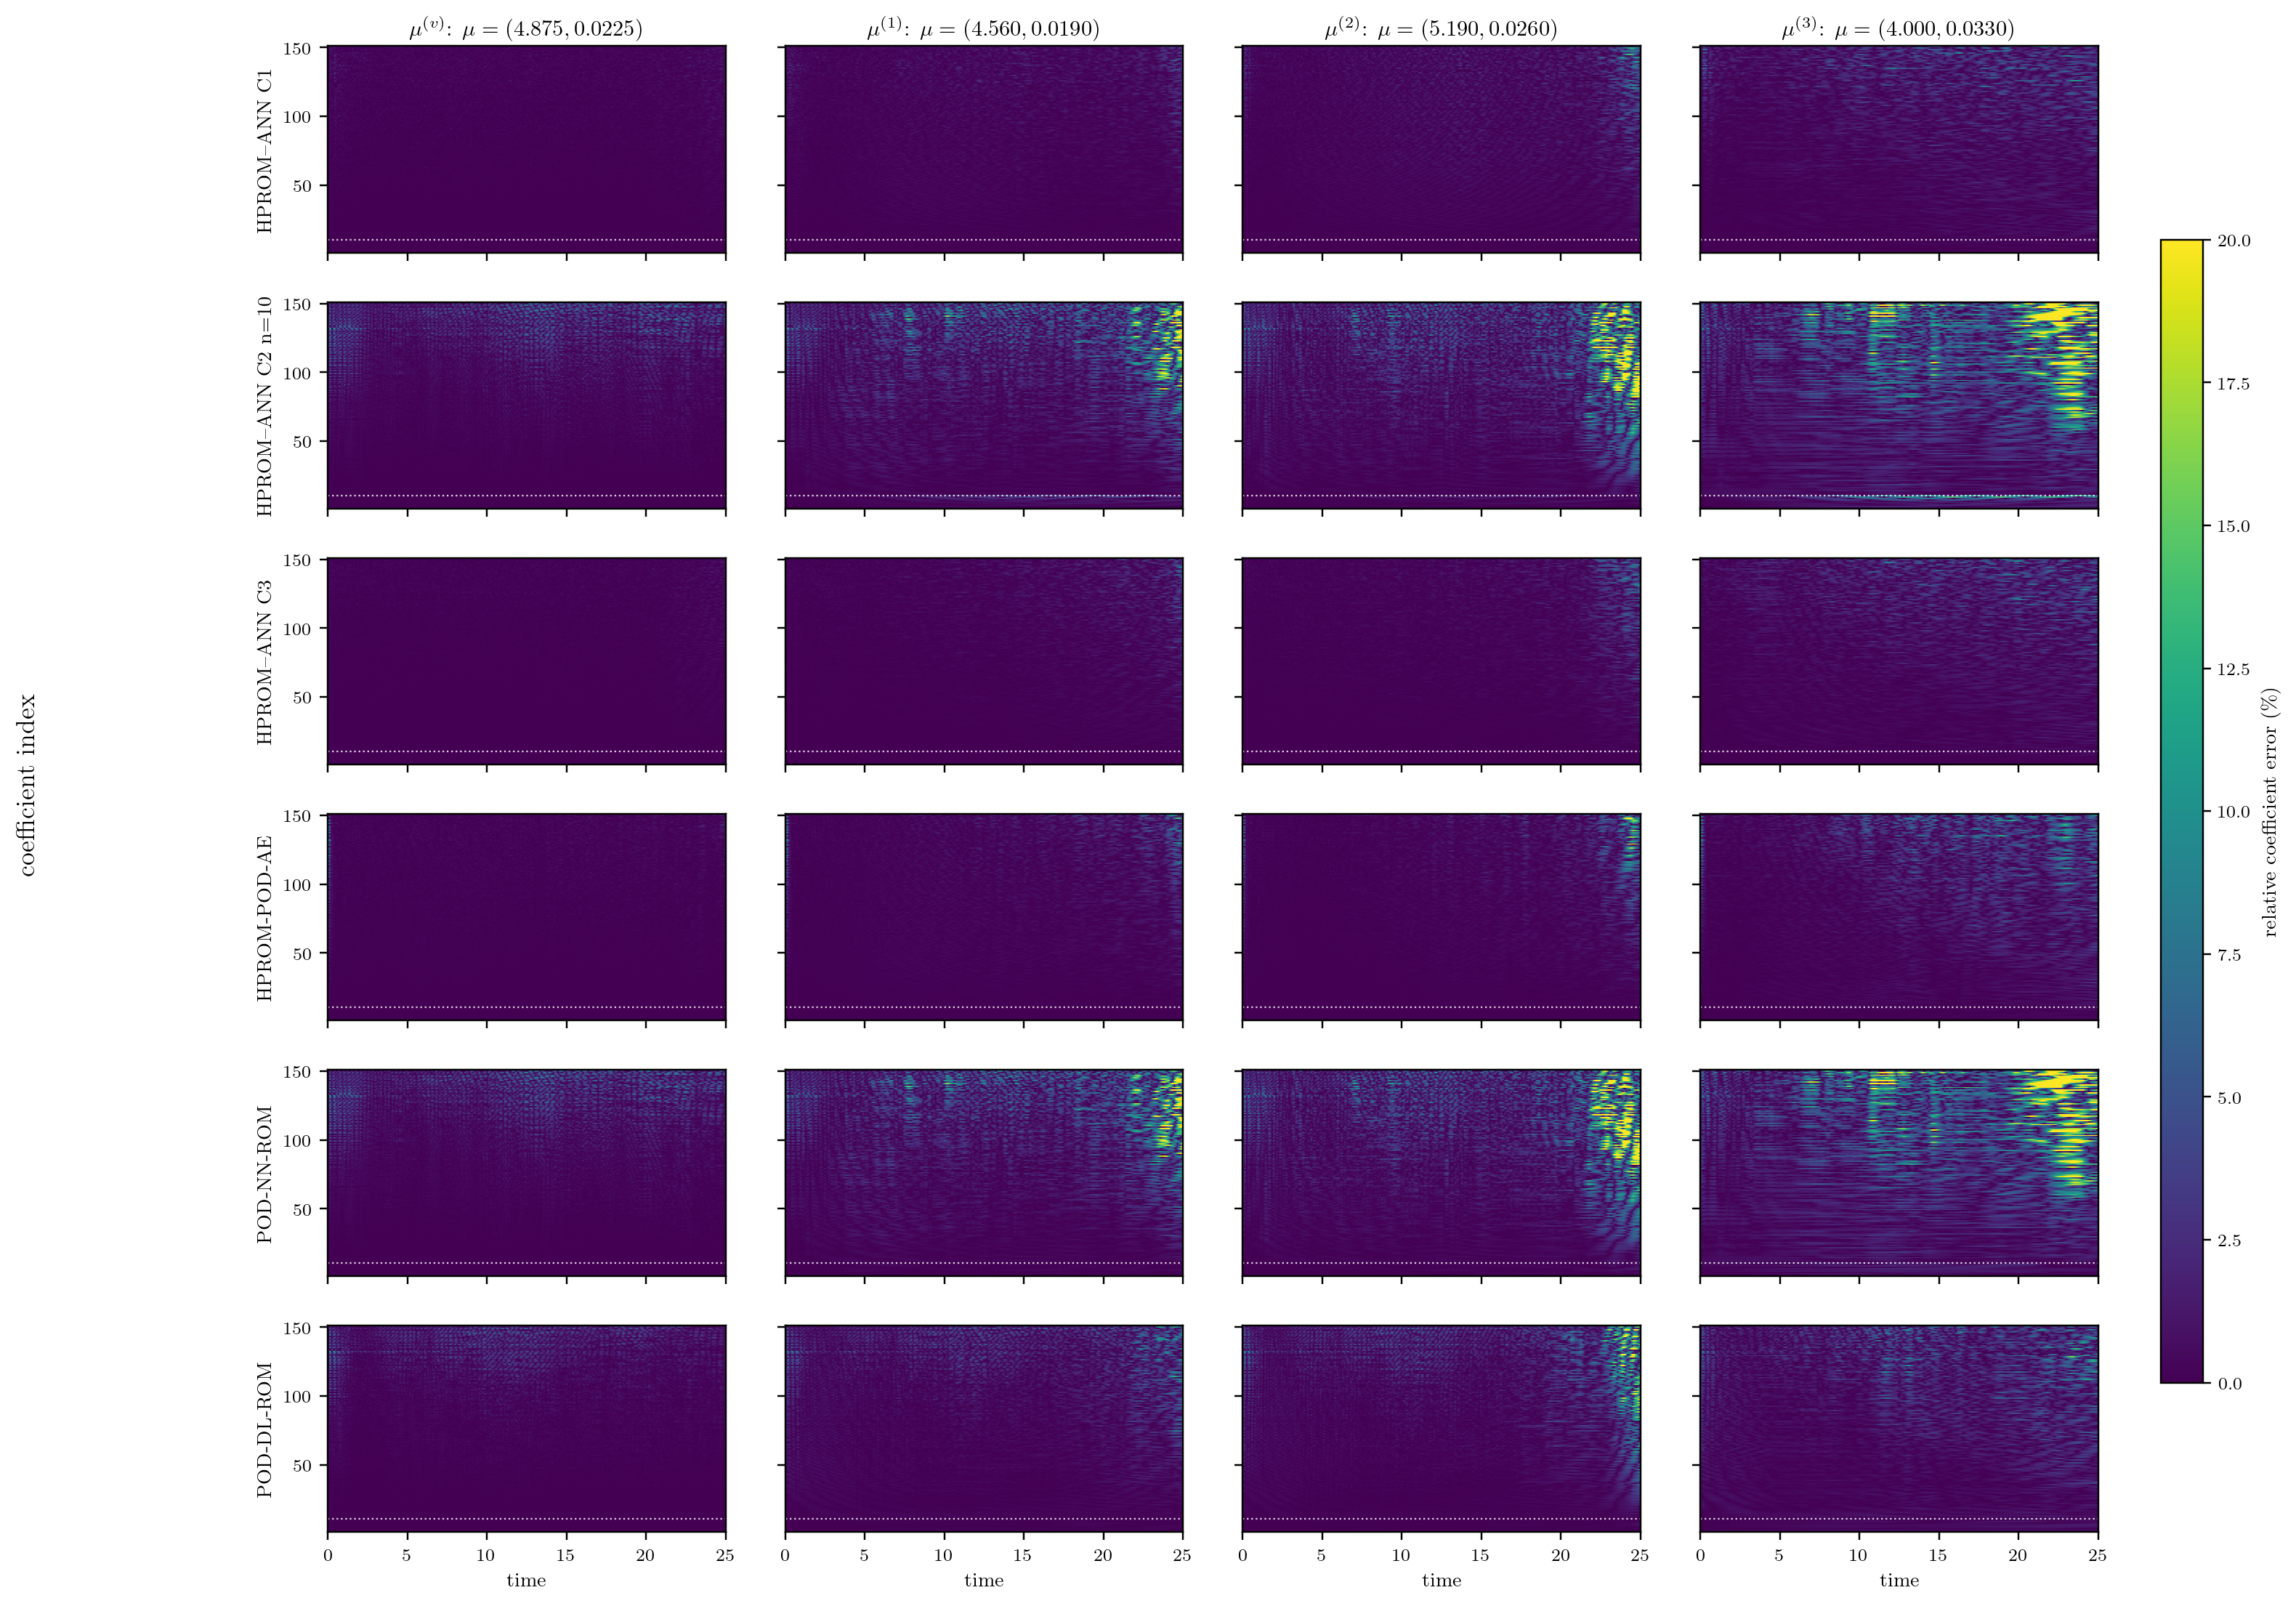
\includegraphics[width=0.98\textwidth]{Figures/hprom_only/hprom_baseline_coeff_rel_heatmaps.png}
\caption{Baseline HPROM time-by-coefficient relative errors against the linear HPROM.  The common \(0\)--\(20\%\)
colour range is exactly the one used in Fig.~\ref{fig:prom-coeff-rel-heatmaps}; hence colour intensities can be
compared directly between the PROM and HPROM panels.}
\label{fig:hprom-coeff-rel-heatmaps}
\end{figure}

\subsection{Case--2 HPROM Diagnostic Sweep}
The Case--2 mechanism can be examined separately from the production comparison by varying the number of residual-solved primary coordinates.  The two endpoints are the direct parameter--time map at $n=0$ and the $151$-coordinate linear HPROM at $n=151$.  For every intermediate value $n\in\{3,5,10,20,30,50\}$, we rebuilt a matched Case--2 ECM rule from the same nine parameter trajectories using $2\%$ global parameter--time stratified residual snapshots, seed 42, and direct dense SVD.  Thus, the intermediate rows are a diagnostic of the coupled choice of primary dimension and matched cubature rule, not a continuation with one fixed sampled residual.

\begin{table}[H]
\centering
\caption{Case--2 HPROM diagnostic state errors $100\norm{\uvec_{\mathrm{HDM}}-\uvec_{\mathrm{ROM}}}_F/\norm{\uvec_{\mathrm{HDM}}}_F$.  The intermediate rows use newly built, matched $2\%$ ECM rules; $n=0$ and $n=151$ are the existing direct-map and linear-HPROM references.  The mean averages $\mub^{(v)},\mub^{(1)},\mub^{(2)}$.}
\label{tab:hprom-case2-n-sweep}
\resizebox{\textwidth}{!}{\begin{tabular}{lrrrrrrr}
\toprule
Solved $n$ & $N_{\rm ECM}$ & $\mu^{(v)}$ & $\mu^{(1)}$ & $\mu^{(2)}$ & Mean & $\mu^{(3)}$ \\
\midrule
0 & -- & 0.508 & 1.834 & 2.479 & 1.607 & 7.401 \\
10 & 901 & 0.505 & 1.902 & 2.120 & 1.509 & 4.257 \\
20 & 1801 & 0.504 & 1.372 & 1.909 & 1.261 & 3.005 \\
30 & 2701 & 0.501 & 1.312 & 1.782 & 1.198 & 3.096 \\
50 & 4442 & 0.498 & 1.226 & 1.543 & 1.089 & 2.822 \\
151 & 5975 & 0.413 & 0.460 & 0.472 & 0.448 & 0.868 \\
\bottomrule
\end{tabular}
}
\end{table}

\begin{figure}[H]
\centering
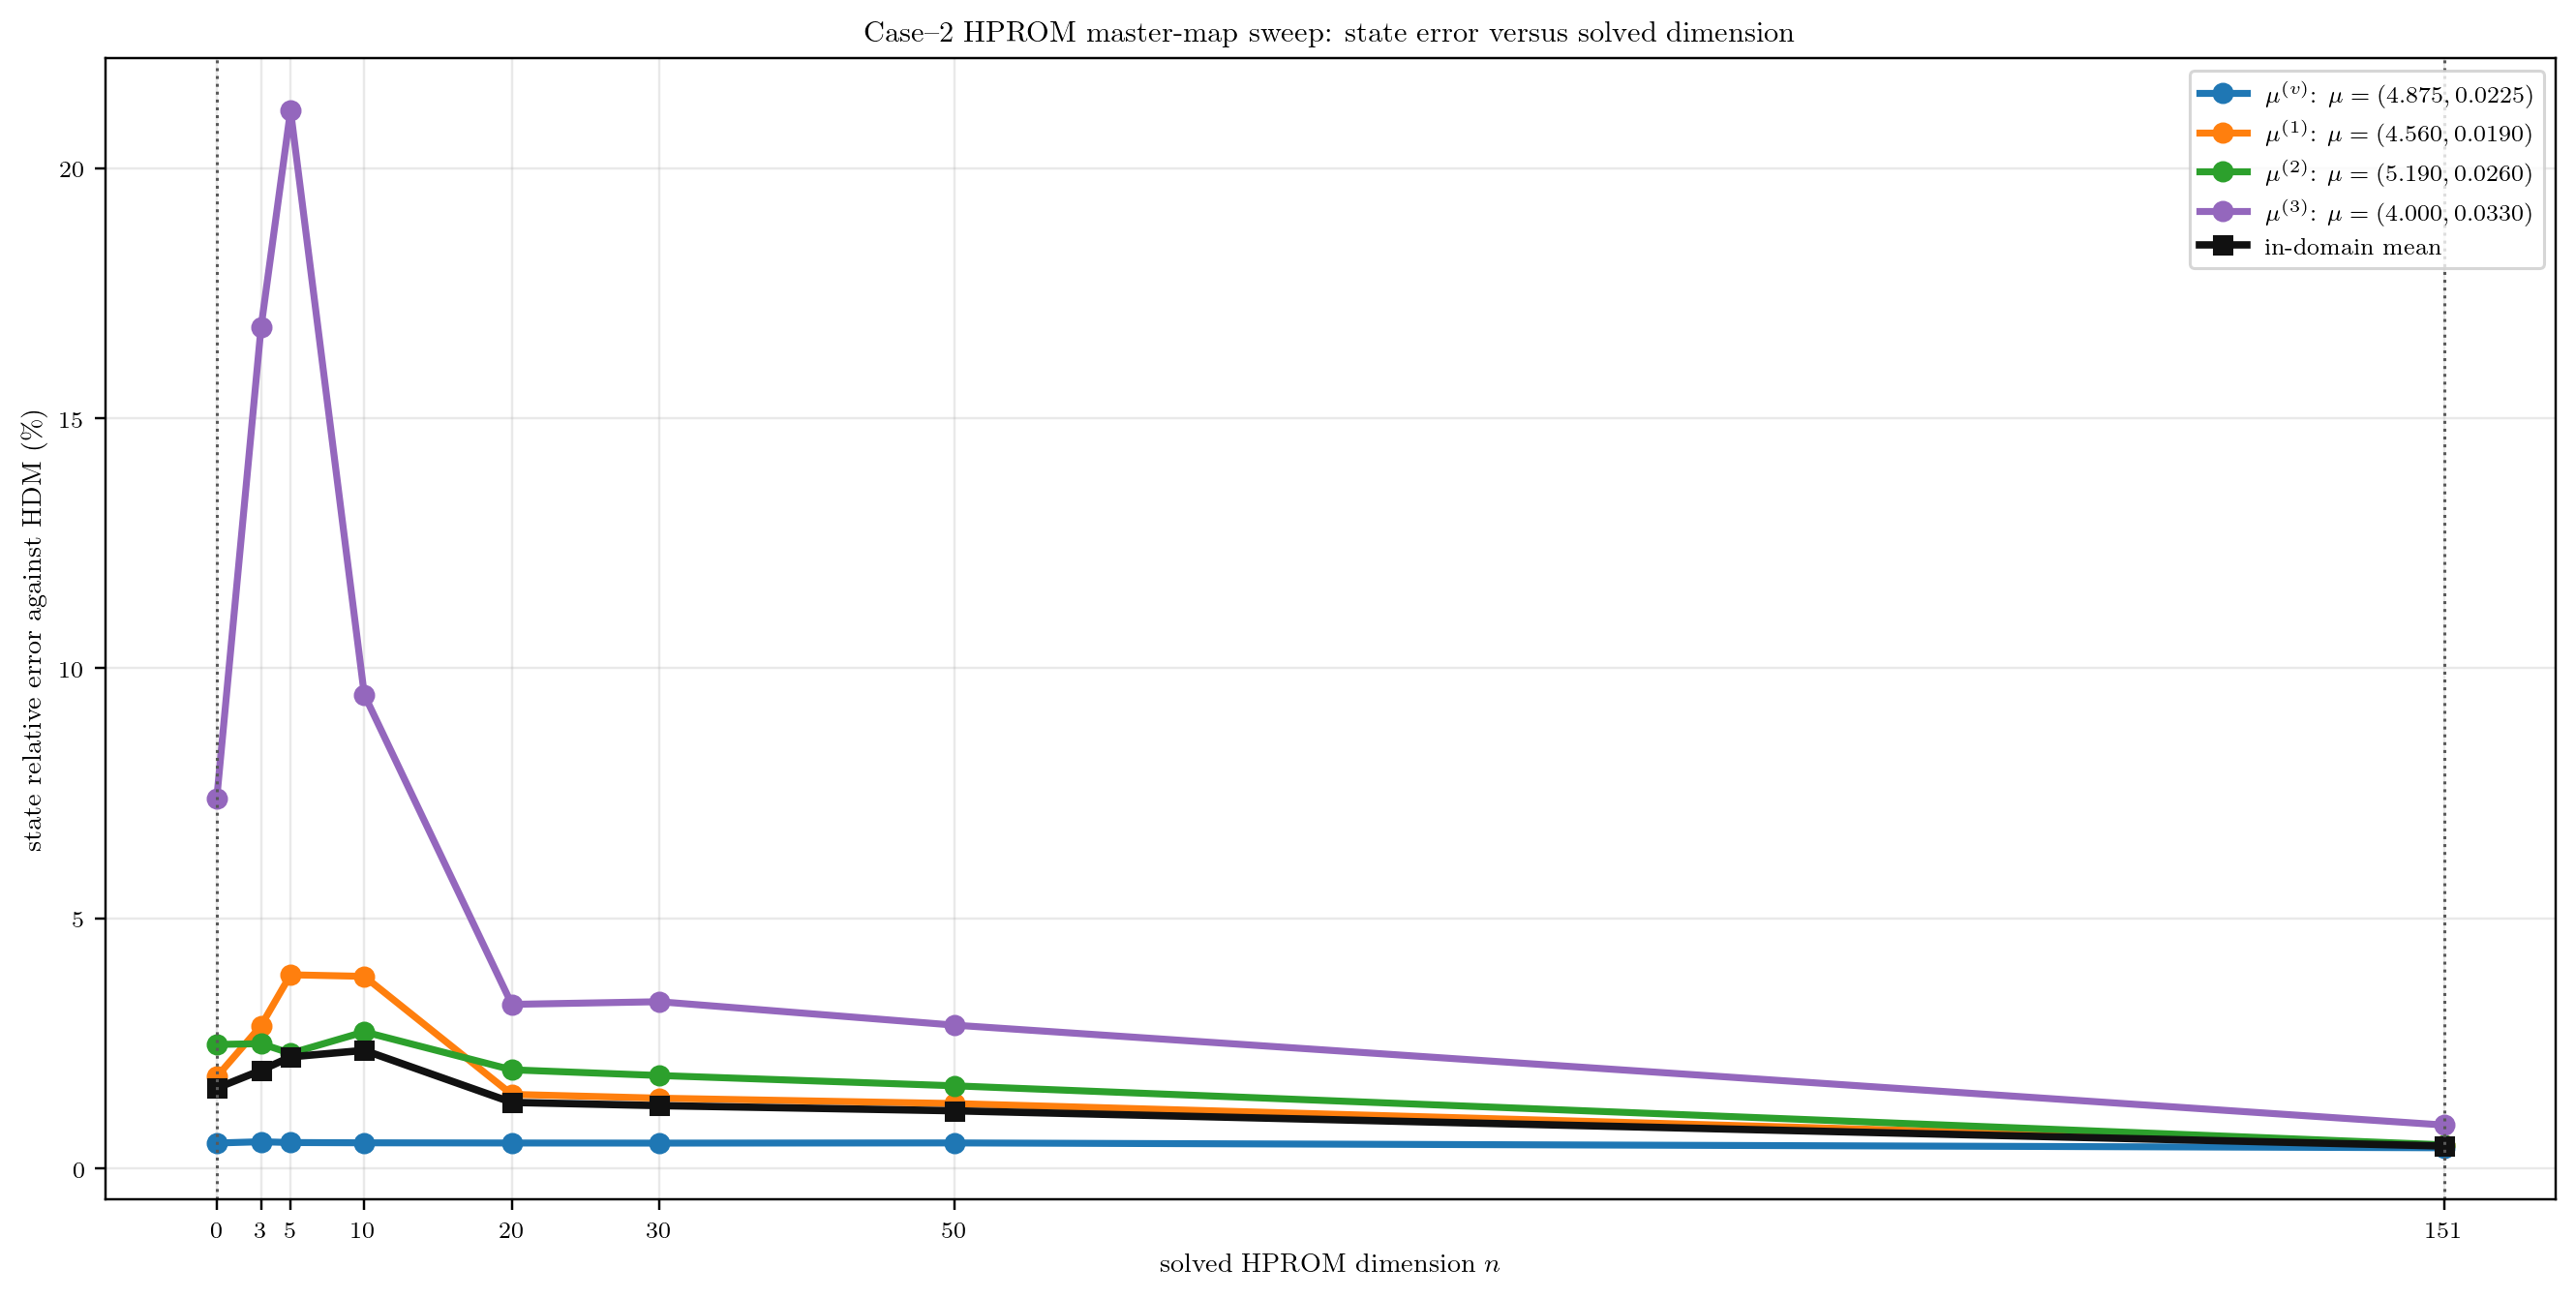
\includegraphics[width=0.98\textwidth]{Figures/hprom_only/hprom_case2_n_sweep_state_errors.png}
\caption{Case--2 HPROM state error as the number $n$ of residual-solved primary coordinates is varied.  Each
intermediate point uses its matched $2\%$ ECM rule.  The dotted horizontal levels are the $151$-coordinate
linear-HPROM errors.}
\label{fig:hprom-case2-n-sweep-state}
\end{figure}

The small-$n$ behavior is non-monotone.  The direct map has an in-domain mean error of $1.607\%$ and an extrapolatory error of $7.401\%$.  Solving three or five coordinates does not reliably improve this result: the corresponding in-domain/extrapolatory pairs are $1.961\%/16.816\%$ and $2.230\%/21.154\%$.  Once $n\geq20$, the matched HPROM errors decrease to $1.321\%/3.280\%$ at $n=20$, $1.256\%/3.334\%$ at $n=30$, and $1.153\%/2.865\%$ at $n=50$.  These values remain above the linear-HPROM reference ($0.448\%/0.868\%$), but show that the degradation is not an unavoidable consequence of solving only a subset of coordinates.

\begin{figure}[H]
\centering
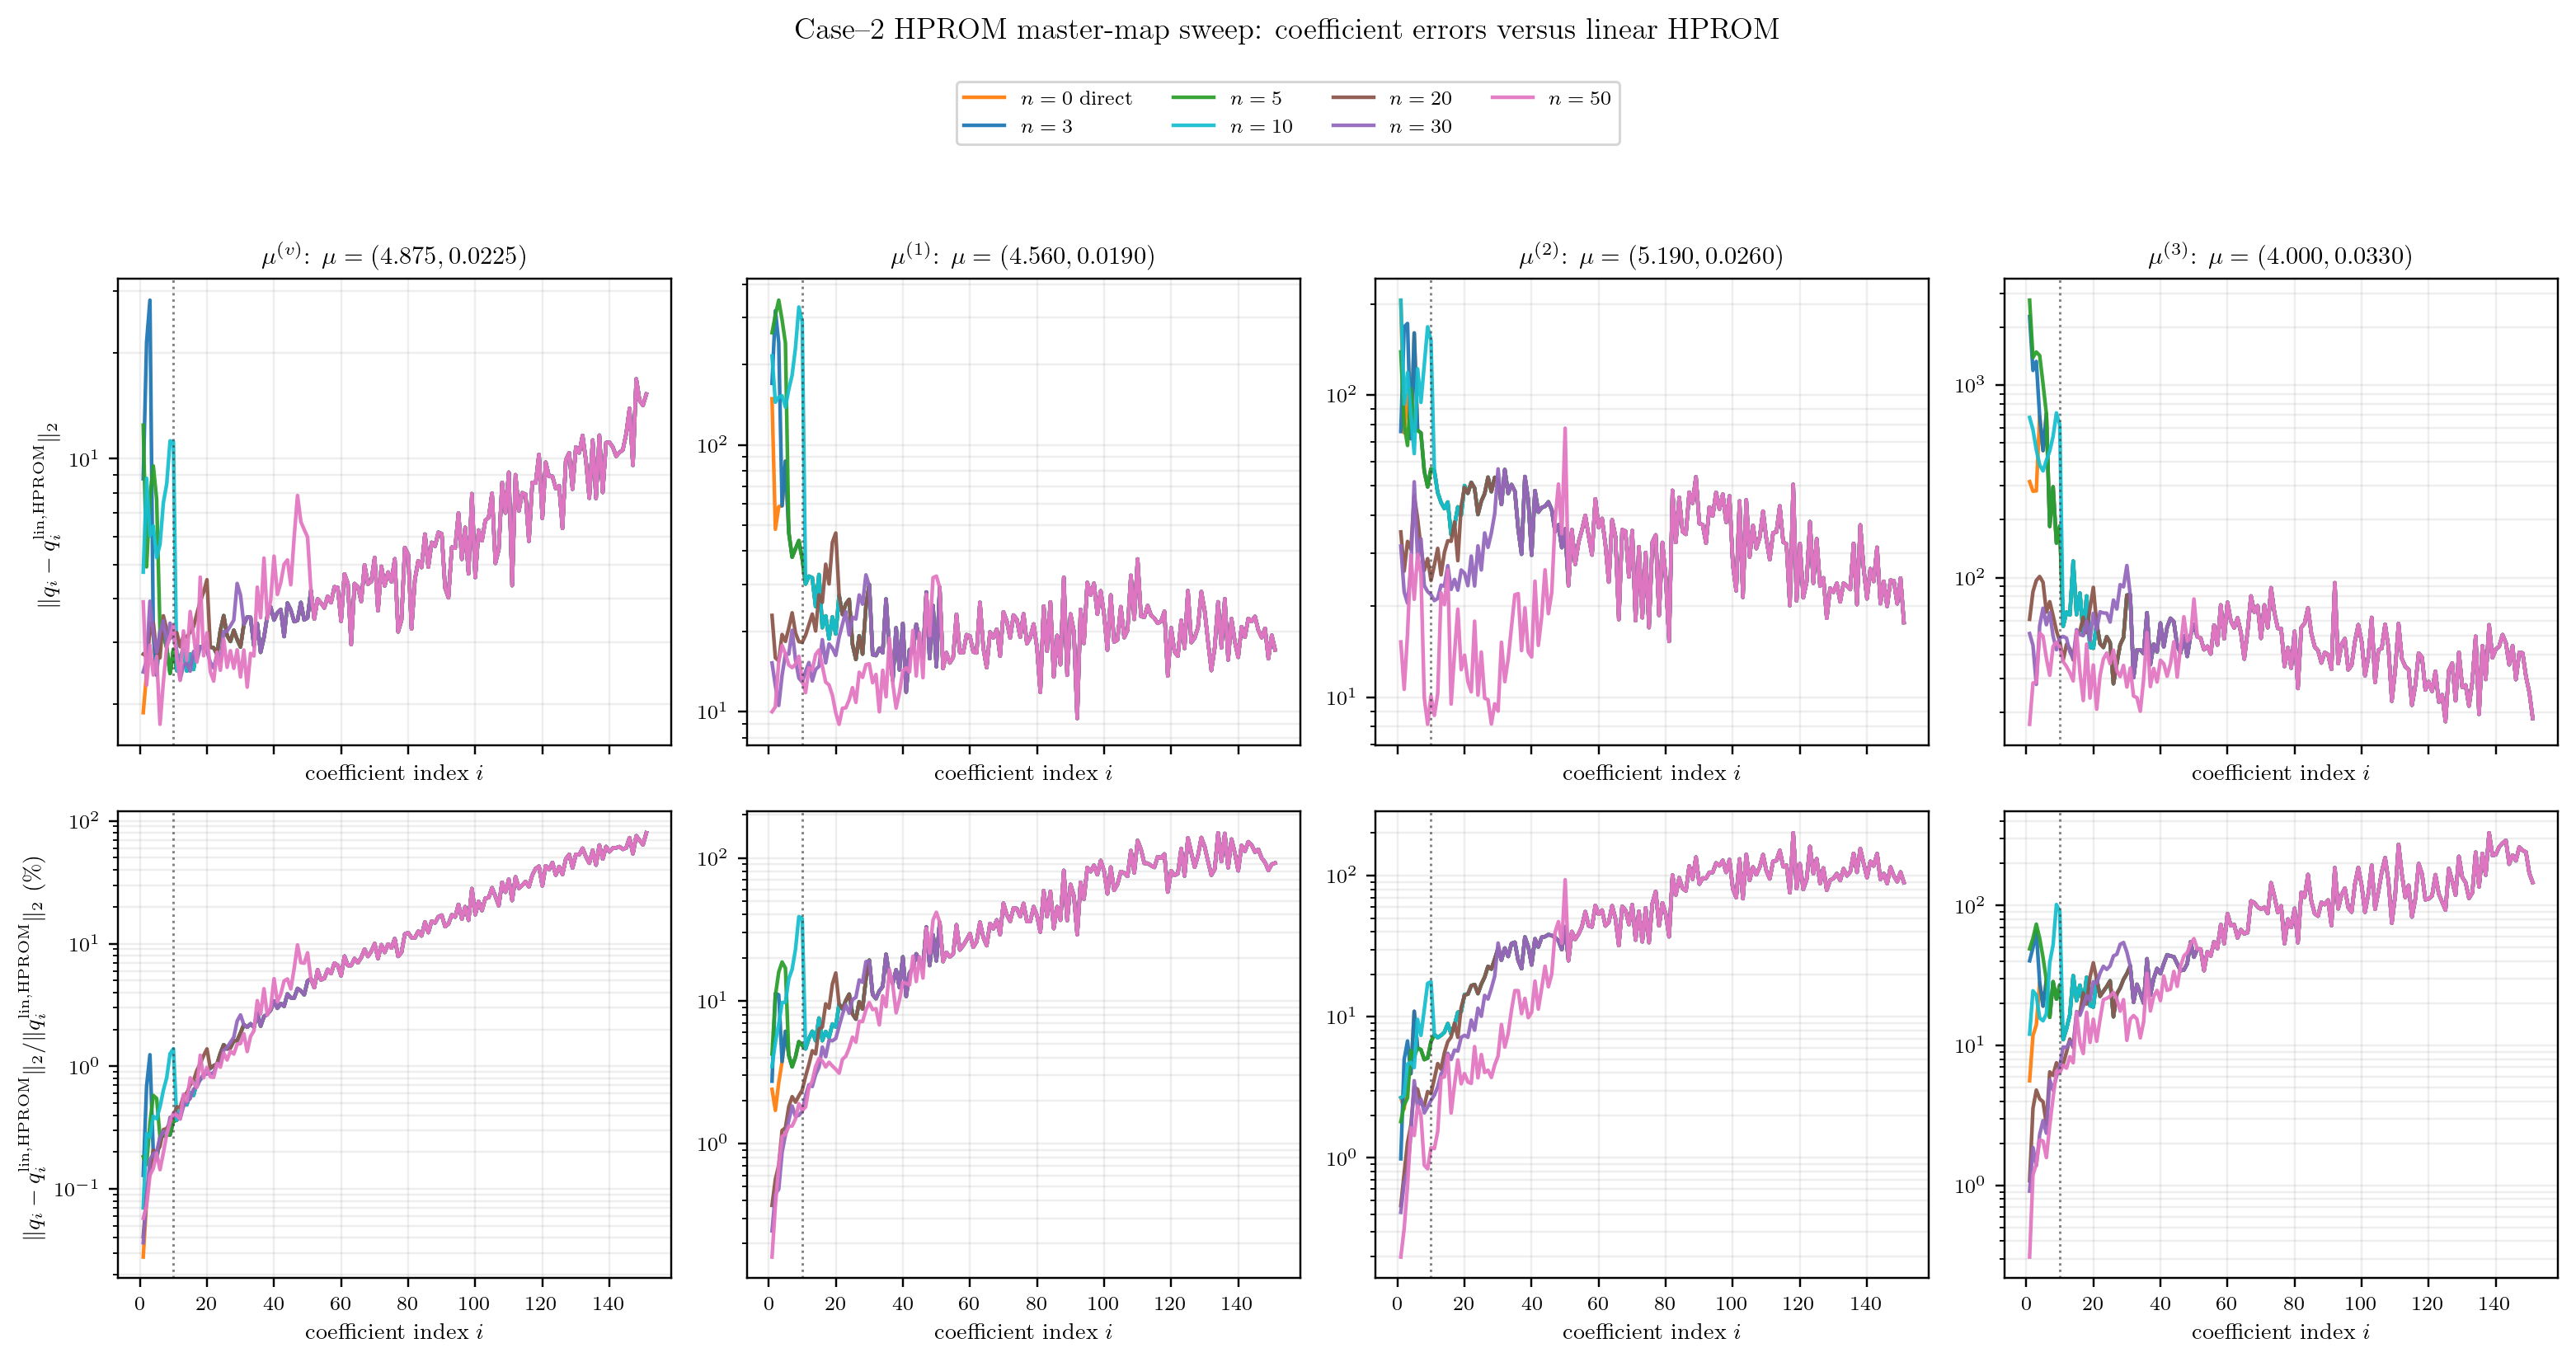
\includegraphics[width=0.98\textwidth]{Figures/hprom_only/hprom_case2_n_sweep_coeff_errors.png}
\caption{Case--2 HPROM coefficient errors for the matched-rule diagnostic sweep.  Top: absolute time-trajectory
error. Bottom: relative error with respect to the linear HPROM.  The dotted vertical line separates the first ten
coordinates.  The $n=151$ linear HPROM is the zero-error reference and is omitted.}
\label{fig:hprom-case2-n-sweep-coeff}
\end{figure}

Figure~\ref{fig:hprom-case2-n-sweep-coeff} shows that the residual solve chiefly reduces errors inside the solved leading block.  The secondary tail remains the output of the same master map, so increasing $n$ moves the boundary of the correction without making the learned tail exact.  The resulting state trend is therefore a coupled consequence of a larger solved subspace and a different sampled residual, rather than a simple monotone interpolation between the two endpoints.

\subsection{Fixed-Rule Tail-Error Sensitivity}
To isolate tail feedback from the changing-rule effect, we fixed the production Case--2 $n=10$ ECM rule ($N_e=901$) and imposed a controlled secondary-coordinate perturbation
$\q_s^{\mathrm{used}}=\q_s^{\mathrm{lin,HPROM}}+\alpha(\widehat{\q}_s-\q_s^{\mathrm{lin,HPROM}})$.
Here $\widehat{\q}_s$ is the master-ANN tail and $\alpha$ scales its actual error direction from zero to $50\%$ of the linear-HPROM tail norm.  The primary coordinates are still obtained by the same sampled LSPG solve.  Stars in Fig.~\ref{fig:hprom-case2-tail-sensitivity} mark the actual master-ANN tail error at each test point.

\begin{table}[H]
\centering
\caption{Fixed-rule Case--2 HPROM tail diagnostic for $n=10$; all error columns are percentages.  The master-ANN tail error is measured against the linear HPROM.  The zero-tail row is the constrained ten-coordinate sampled solve with the exact linear-HPROM tail; it is not the $151$-coordinate linear-HPROM solution.}
\label{tab:hprom-case2-tail-sensitivity}
\resizebox{0.92\textwidth}{!}{\begin{tabular}{lrrrrr}
\toprule
Point & ANN tail error & $e_u$ at exact tail & $e_u$ at ANN tail & $e_{q_p}$ at ANN tail & $e_{q_{151}}$ at ANN tail \\
\midrule
$\mu^{(v)}$ & 4.353 & 0.452 & 0.512 & 0.184 & 0.941 \\
$\mu^{(1)}$ & 14.695 & 0.564 & 4.516 & 10.164 & 10.420 \\
$\mu^{(2)}$ & 21.740 & 0.475 & 2.895 & 4.865 & 6.538 \\
$\mu^{(3)}$ & 38.799 & 1.077 & 13.098 & 30.445 & 30.777 \\
\bottomrule
\end{tabular}
}
\end{table}

\begin{figure}[H]
\centering
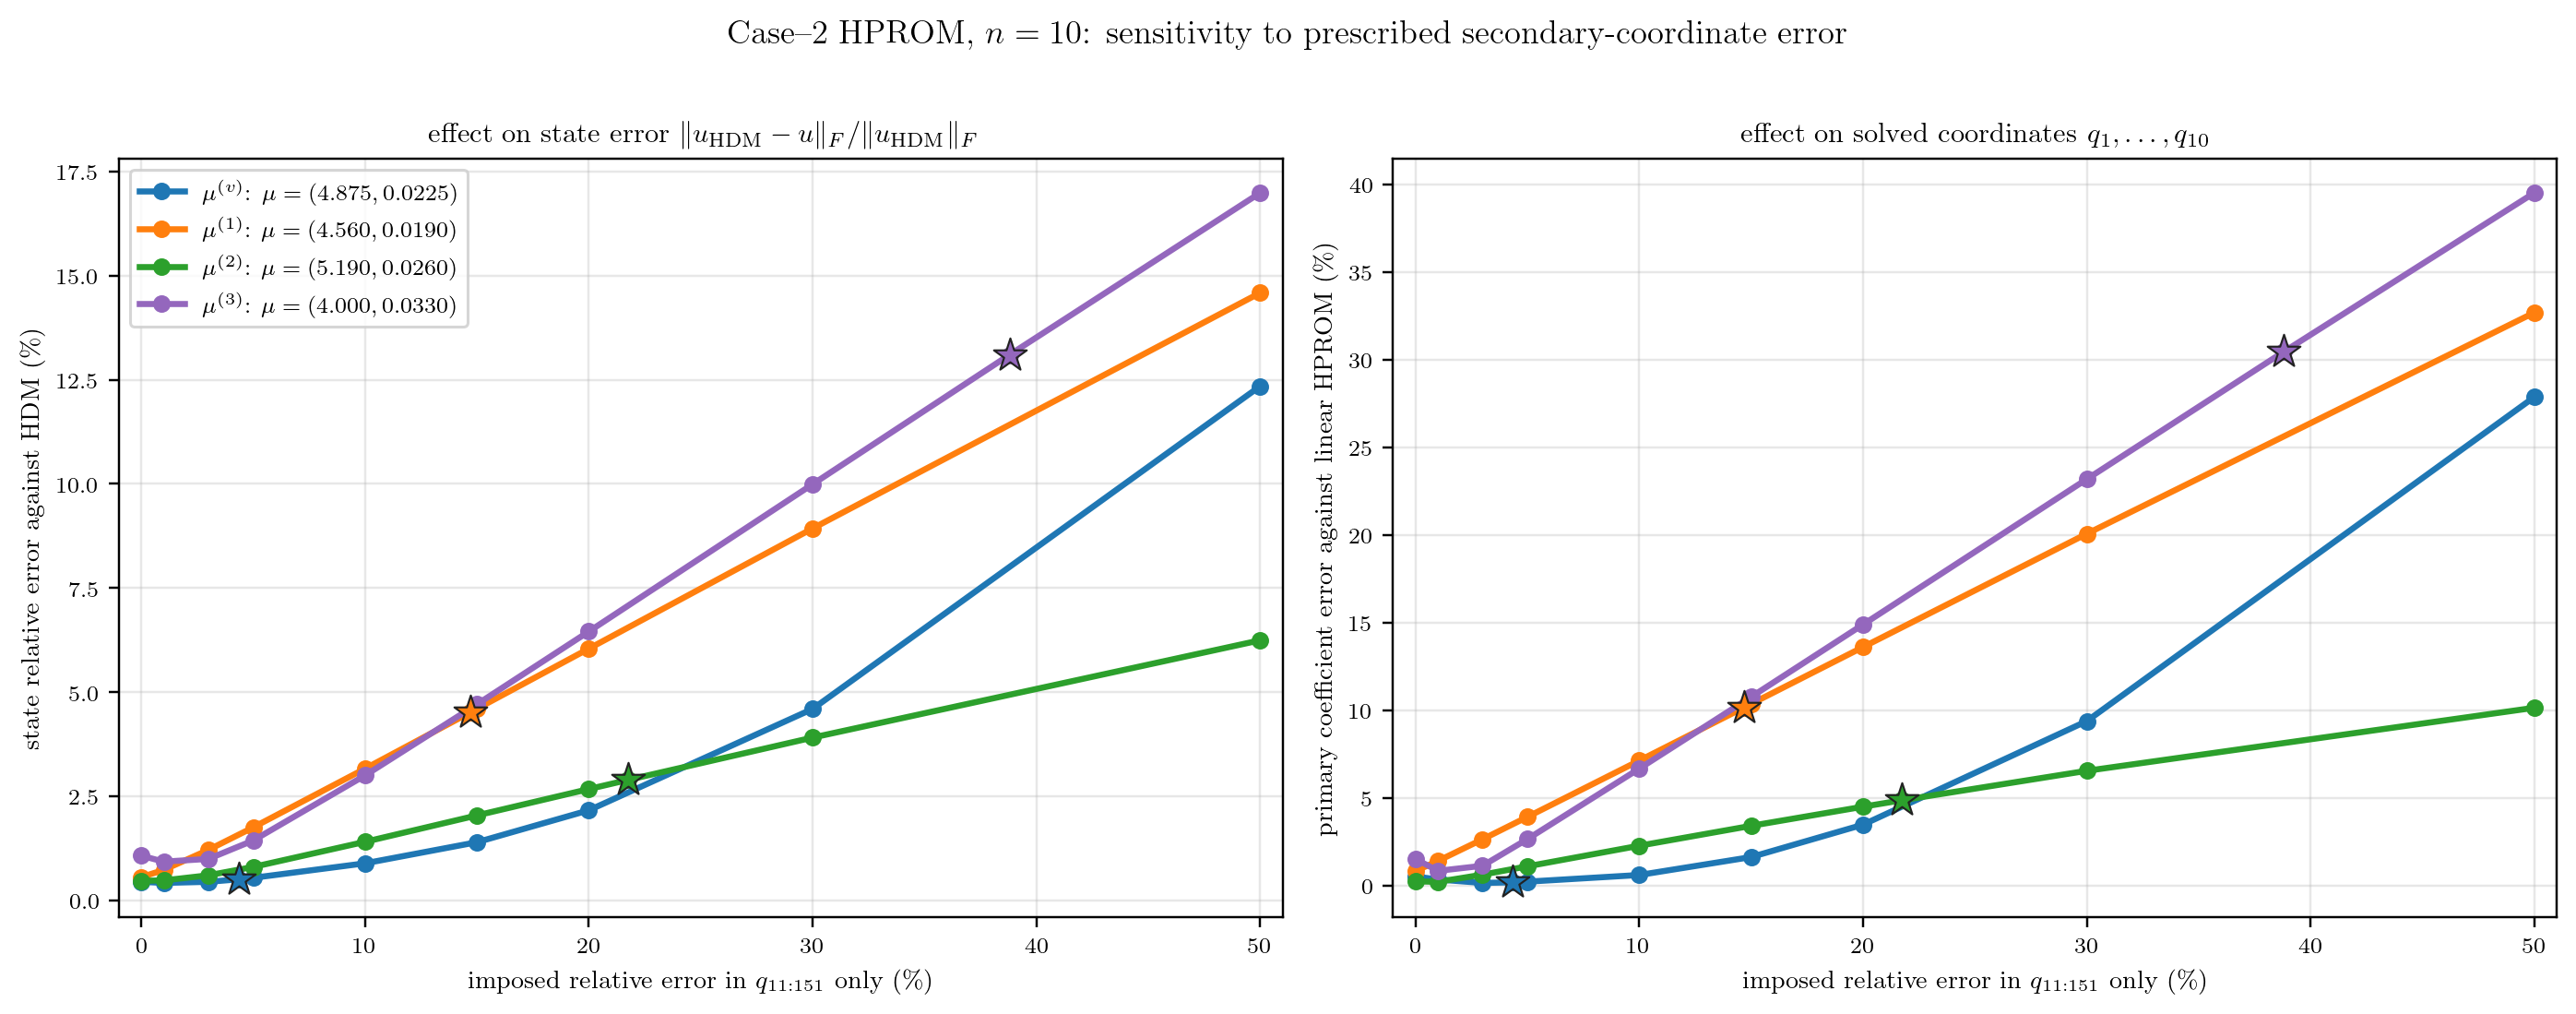
\includegraphics[width=0.98\textwidth]{Figures/hprom_only/hprom_case2_secondary_sensitivity_state_and_primary_error.png}
\caption{Fixed-rule sensitivity of Case--2 HPROM with $n=10$ to secondary-coordinate error.  Left: state error against the HDM.  Right: error in the ten solved primary coordinates against the linear HPROM.  Stars identify the actual master-ANN tail errors.}
\label{fig:hprom-case2-tail-sensitivity}
\end{figure}

The fixed-rule result establishes direct residual feedback.  Even an exact linear-HPROM tail leaves a nonzero zero-tail baseline because a constrained ten-coordinate sampled solve is not the full $151$-coordinate linear-HPROM problem.  Additional tail error then changes the solved primary coordinates: at off-grid point $\mub^{(1)}$, a $14.695\%$ master-ANN tail error produces a $10.164\%$ primary-coordinate error and a $4.516\%$ state error; at the extrapolatory point, a $38.799\%$ tail error produces $30.445\%$ and $13.098\%$, respectively.  Hence Case 2 is not a passive reconstruction map: its learned tail enters the online residual and can shift the coordinates that are nominally solved intrusively.

\section{Effect of HPROM Coefficient-Data Enrichment}
The HPROM enrichment campaign uses the same 36 Latin-hypercube parameter locations as the PROM study: 18 interior
points and 18 points in the 25\% expanded exterior rectangle, with seed 42.  The fixed basis, the 2\%
parameter--time sampling ratio, direct dense SVD, and the nine baseline parameter locations used to construct each
nonlinear ECM rule are retained.  The nonlinear residual maps do change with the retrained neural networks, so a
rule is rebuilt for each enriched learned model, but no new HDM trajectory or residual-training parameter location
is introduced.  Consequently, this experiment isolates the effect of enlarging the linear-HPROM coefficient teacher
data from 9 to 45 trajectories.

\begin{table}[H]
\centering
\caption{Reported coefficient-space training and validation errors for the HPROM learned maps before and after
coefficient-data enrichment.  Values are relative Frobenius percentages.  The baseline records use their original
internal held-out snapshot split; the enriched master-map record uses the two separate validation trajectories, so
the validation columns are useful diagnostics but are not a strictly paired model-selection protocol.}
\label{tab:hprom-enrichment-training}
\resizebox{0.94\textwidth}{!}{\begin{tabular}{lrr|rrr}
\toprule
Model & Base train $e_q$ (\%) & Base val. $e_q$ (\%) & Enriched train $e_q$ (\%) & Enriched val. $e_q$ (\%) & Val. reduction (\%) \\
\midrule
HPROM--ANN Case 1 & 0.992 & 1.101 & 0.358 & 0.373 & 66.1 \\
Master POD--NN--ROM (Case 2 tail source) & 0.975 & 1.124 & 0.404 & 0.489 & 56.5 \\
HPROM--ANN Case 3 & 0.491 & 0.577 & 0.202 & 0.234 & 59.4 \\
HPROM-POD-AE ($n_z=10$) & 0.098 & 0.119 & 0.049 & 0.066 & 45.0 \\
POD--DL--ROM ($n_z=10$) & 0.624 & 0.744 & 0.130 & 0.142 & 80.9 \\
\bottomrule
\end{tabular}
}
\end{table}

The training diagnostics improve for every intrinsic closure.  For example, the reported Case 1 validation error
decreases from \(1.101\%\) to \(0.373\%\), Case 3 decreases from \(0.577\%\) to \(0.234\%\), and the master
parameter--time map decreases from \(1.124\%\) to \(0.489\%\).  The online comparisons below are the decisive
test, because all four points are kept out of both training campaigns.

\begin{table}[H]
\centering
\caption{Baseline and enriched state errors for the learned models trained on linear-HPROM coefficient data.
\(100\norm{\uvec_{\mathrm{HDM}}-\uvec_{\mathrm{ROM}}}_F/\norm{\uvec_{\mathrm{HDM}}}_F\).  Each mean averages
\(\mub^{(v)},\mub^{(1)},\mub^{(2)}\).  The linear HPROM is identical in both columns because its basis and ECM rule
are fixed.  The horizontal rule separates residual-evaluating HPROMs from the two non-intrusive direct maps.}
\label{tab:hprom-enrichment-online}
\resizebox{\textwidth}{!}{\begin{tabular}{lrrrrr|rrrrr}
\toprule
& \multicolumn{5}{c|}{Baseline (9 trajectories)} & \multicolumn{5}{c}{Enriched (9+36 trajectories)} \\
Model & $\mu^{(v)}$ & $\mu^{(1)}$ & $\mu^{(2)}$ & Mean & $\mu^{(3)}$ & $\mu^{(v)}$ & $\mu^{(1)}$ & $\mu^{(2)}$ & Mean & $\mu^{(3)}$ \\
\midrule
Linear HPROM & 0.413 & 0.460 & 0.472 & 0.448 & 0.868 & 0.413 & 0.460 & 0.472 & 0.448 & 0.868 \\
HPROM--ANN Case 1 & 0.408 & 0.521 & 0.670 & 0.533 & 1.578 & 0.413 & 0.459 & 0.471 & 0.448 & 0.870 \\
HPROM--ANN Case 2 ($n=10$) & 0.505 & 1.904 & 2.121 & 1.510 & 4.272 & 0.422 & 0.465 & 0.485 & 0.457 & 0.912 \\
HPROM--ANN Case 3 & 0.404 & 0.513 & 0.563 & 0.494 & 1.374 & 0.410 & 0.454 & 0.470 & 0.445 & 0.875 \\
HPROM-POD-AE ($n_z=10$) & 0.417 & 0.548 & 0.662 & 0.542 & 1.846 & 0.435 & 0.478 & 0.488 & 0.467 & 0.874 \\
\midrule
POD--NN--ROM & 0.508 & 1.834 & 2.479 & 1.607 & 7.401 & 0.423 & 0.466 & 0.487 & 0.458 & 0.926 \\
POD--DL--ROM ($n_z=10$) & 0.451 & 1.483 & 1.498 & 1.144 & 4.753 & 0.414 & 0.460 & 0.473 & 0.449 & 0.869 \\
\bottomrule
\end{tabular}
}
\end{table}

\begin{figure}[H]
\centering
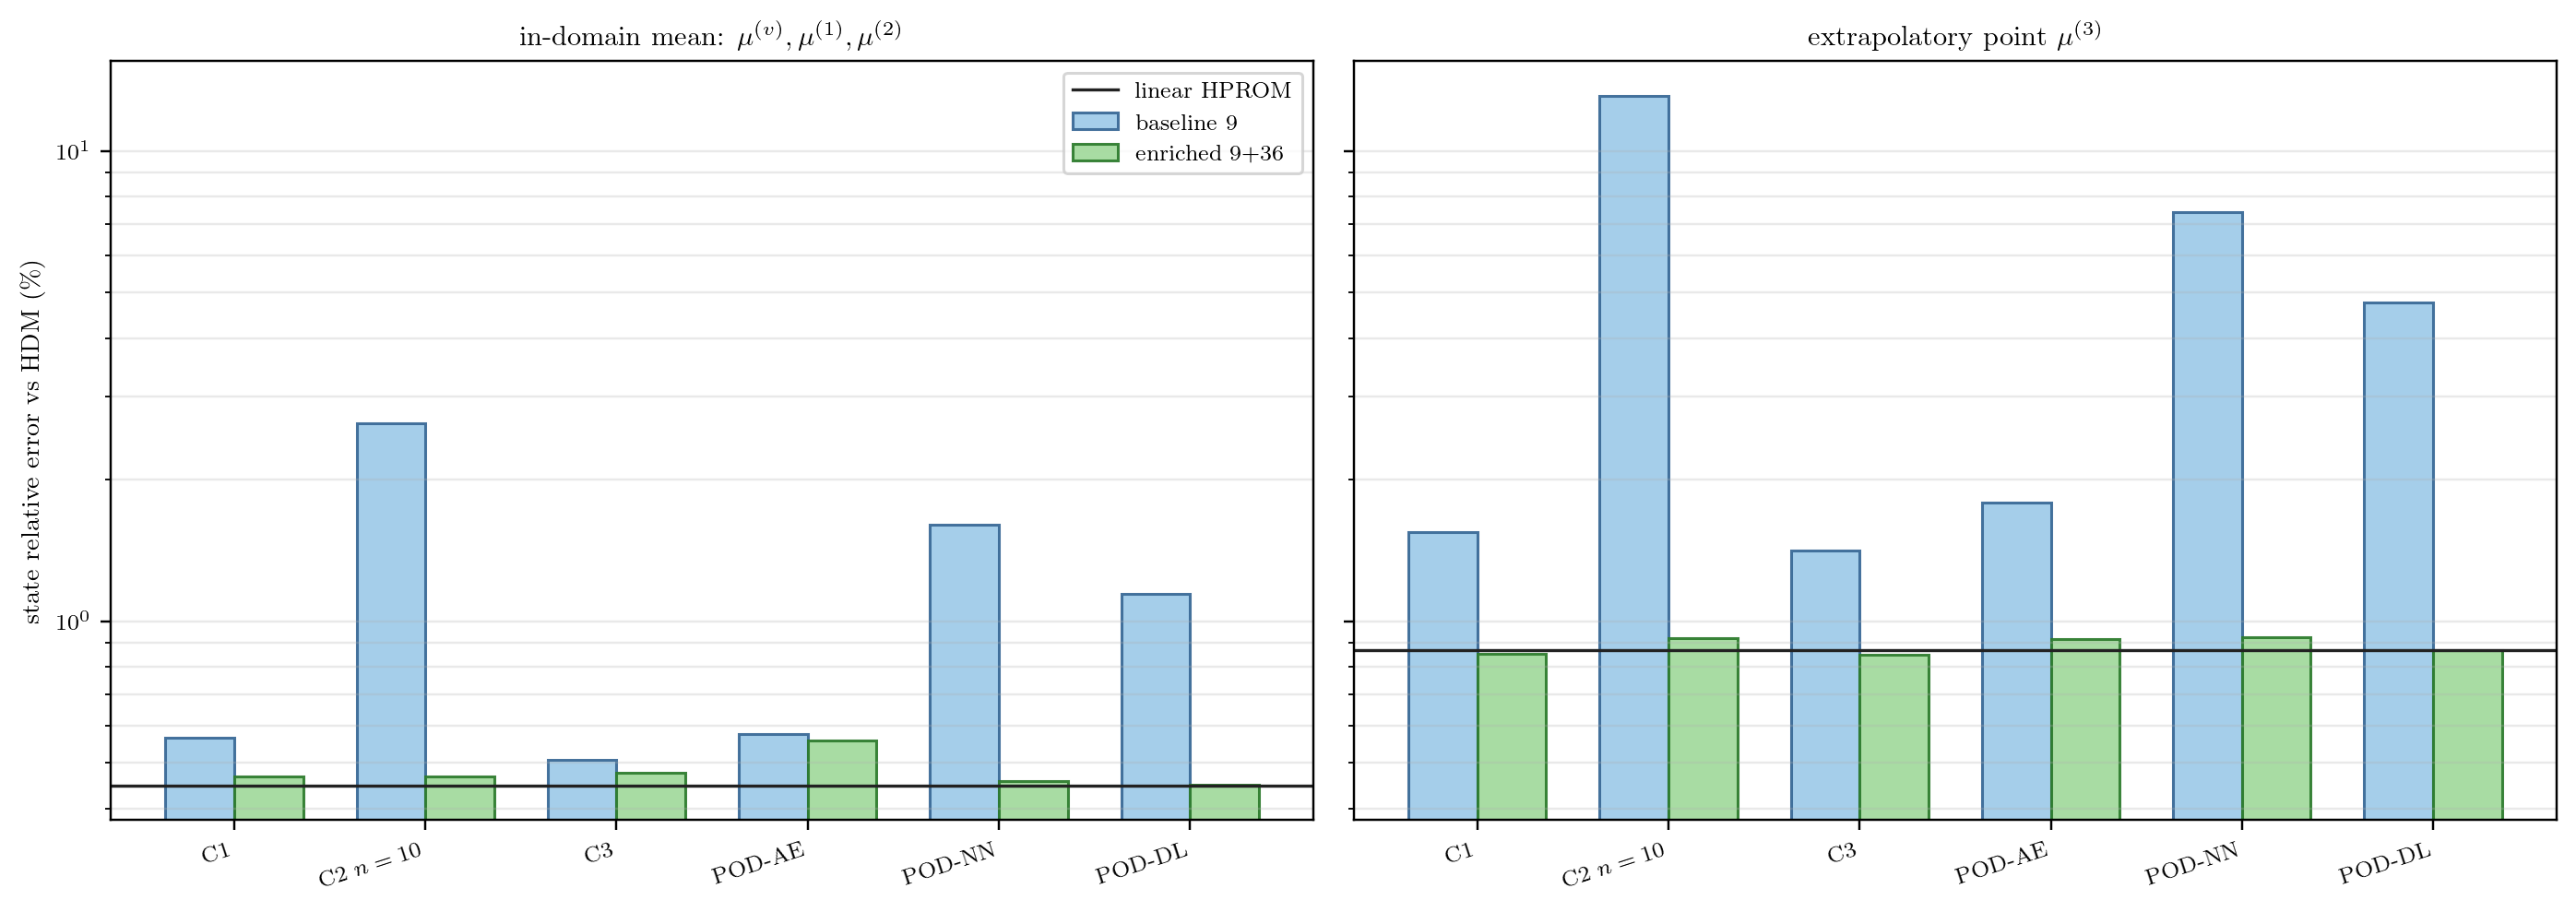
\includegraphics[width=0.98\textwidth]{Figures/hprom_only/hprom_enrichment_state_error_comparison.png}
\caption{Effect of HPROM coefficient-data enrichment on state error.  The black level is the fixed linear HPROM
reference; logarithmic axes make both the baseline Case--2 degradation and the enriched recovery visible.}
\label{fig:hprom-enrichment-state}
\end{figure}

\begin{figure}[H]
\centering
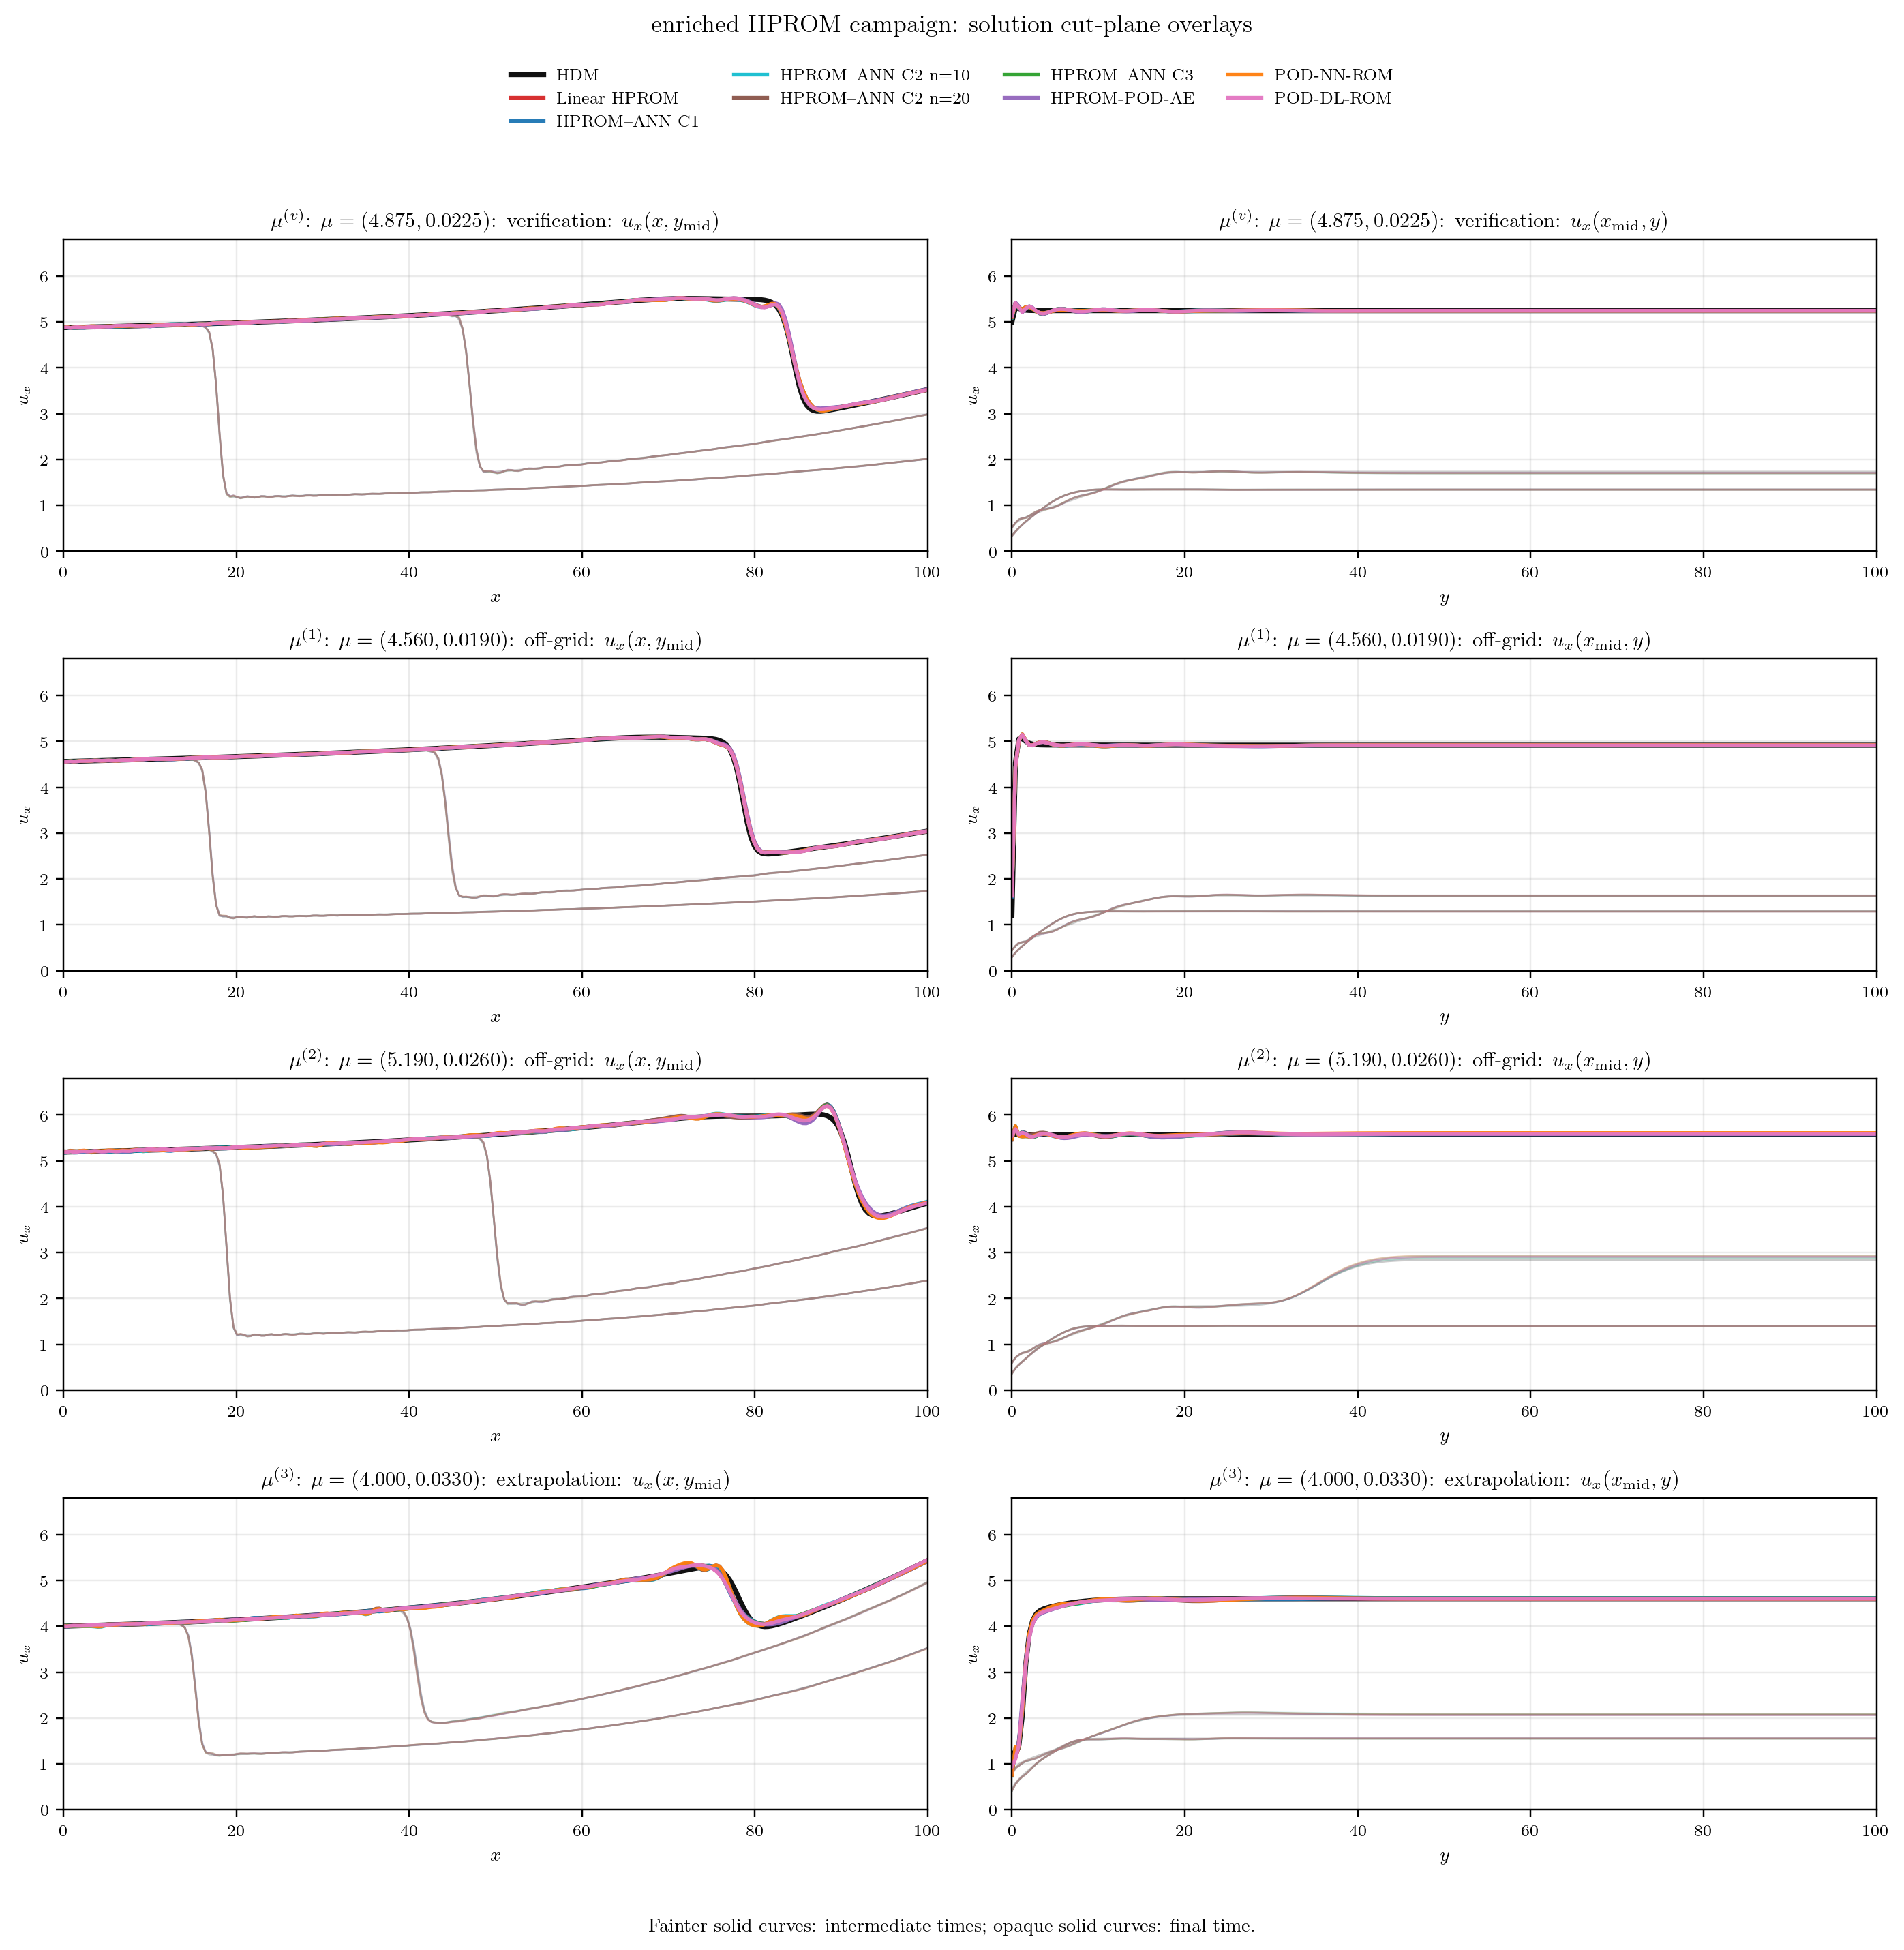
\includegraphics[width=0.98\textwidth]{Figures/hprom_only/hprom_enriched_solution_overlays.png}
\caption{Enriched HPROM solution cut-plane comparison against the HDM.  The same seven online models and the same
shared state range as in Fig.~\ref{fig:hprom-solution-overlays} are used.  Fainter solid curves are intermediate
times and opaque solid curves are final-time traces; model identity is carried only by colour.}
\label{fig:hprom-enriched-solution-overlays}
\end{figure}

The baseline sensitivity of Case 2 disappears after enrichment.  At \(n=10\), its in-domain mean state error falls
from \(2.641\%\) to \(0.468\%\), and the extrapolatory error falls from \(13.098\%\) to \(0.921\%\).  The latter is
close to the \(0.868\%\) linear HPROM reference.  Solving 20 coordinates remains slightly better in coefficient
space, but no longer provides the qualitative rescue that was needed with only nine trajectories.  Case 1 and
Case 3 also remain close to the fixed linear HPROM level, while PROM--POD--AE stays accurate but retains a modest
gap at the first off-grid point.

\begin{table}[H]
\centering
\caption{Baseline and enriched coefficient errors against the corresponding fixed \(n_{\mathrm{tot}}=151\) linear
HPROM coefficient trajectory.  Values are relative Frobenius percentages over all coefficients and all time
steps.  The horizontal rule separates residual-evaluating HPROMs from the two non-intrusive direct maps.}
\label{tab:hprom-enrichment-coeff}
\resizebox{\textwidth}{!}{\begin{tabular}{lrrrrr|rrrrr}
\toprule
& \multicolumn{5}{c|}{Baseline (9 trajectories)} & \multicolumn{5}{c}{Enriched (9+36 trajectories)} \\
Model & $\mu^{(v)}$ & $\mu^{(1)}$ & $\mu^{(2)}$ & Mean & $\mu^{(3)}$ & $\mu^{(v)}$ & $\mu^{(1)}$ & $\mu^{(2)}$ & Mean & $\mu^{(3)}$ \\
\midrule
Linear HPROM & 0.000 & 0.000 & 0.000 & 0.000 & 0.000 & 0.000 & 0.000 & 0.000 & 0.000 & 0.000 \\
HPROM--ANN Case 1 & 0.275 & 0.751 & 1.342 & 0.789 & 2.825 & 0.170 & 0.305 & 0.442 & 0.306 & 0.584 \\
HPROM--ANN Case 2 ($n=10$) & 0.941 & 10.420 & 6.538 & 5.966 & 30.777 & 0.469 & 0.377 & 0.546 & 0.464 & 0.876 \\
HPROM--ANN Case 3 & 0.240 & 0.734 & 0.907 & 0.627 & 2.544 & 0.202 & 0.366 & 0.269 & 0.279 & 0.550 \\
HPROM-POD-AE ($n_z=10$) & 0.365 & 0.936 & 1.160 & 0.820 & 3.950 & 0.599 & 0.919 & 0.449 & 0.656 & 1.177 \\
\midrule
POD--NN--ROM & 0.929 & 4.192 & 5.642 & 3.588 & 17.433 & 0.341 & 0.300 & 0.396 & 0.345 & 0.752 \\
POD--DL--ROM ($n_z=10$) & 0.616 & 3.334 & 3.291 & 2.413 & 11.101 & 0.096 & 0.093 & 0.116 & 0.102 & 0.243 \\
\bottomrule
\end{tabular}
}
\end{table}

\begin{figure}[H]
\centering
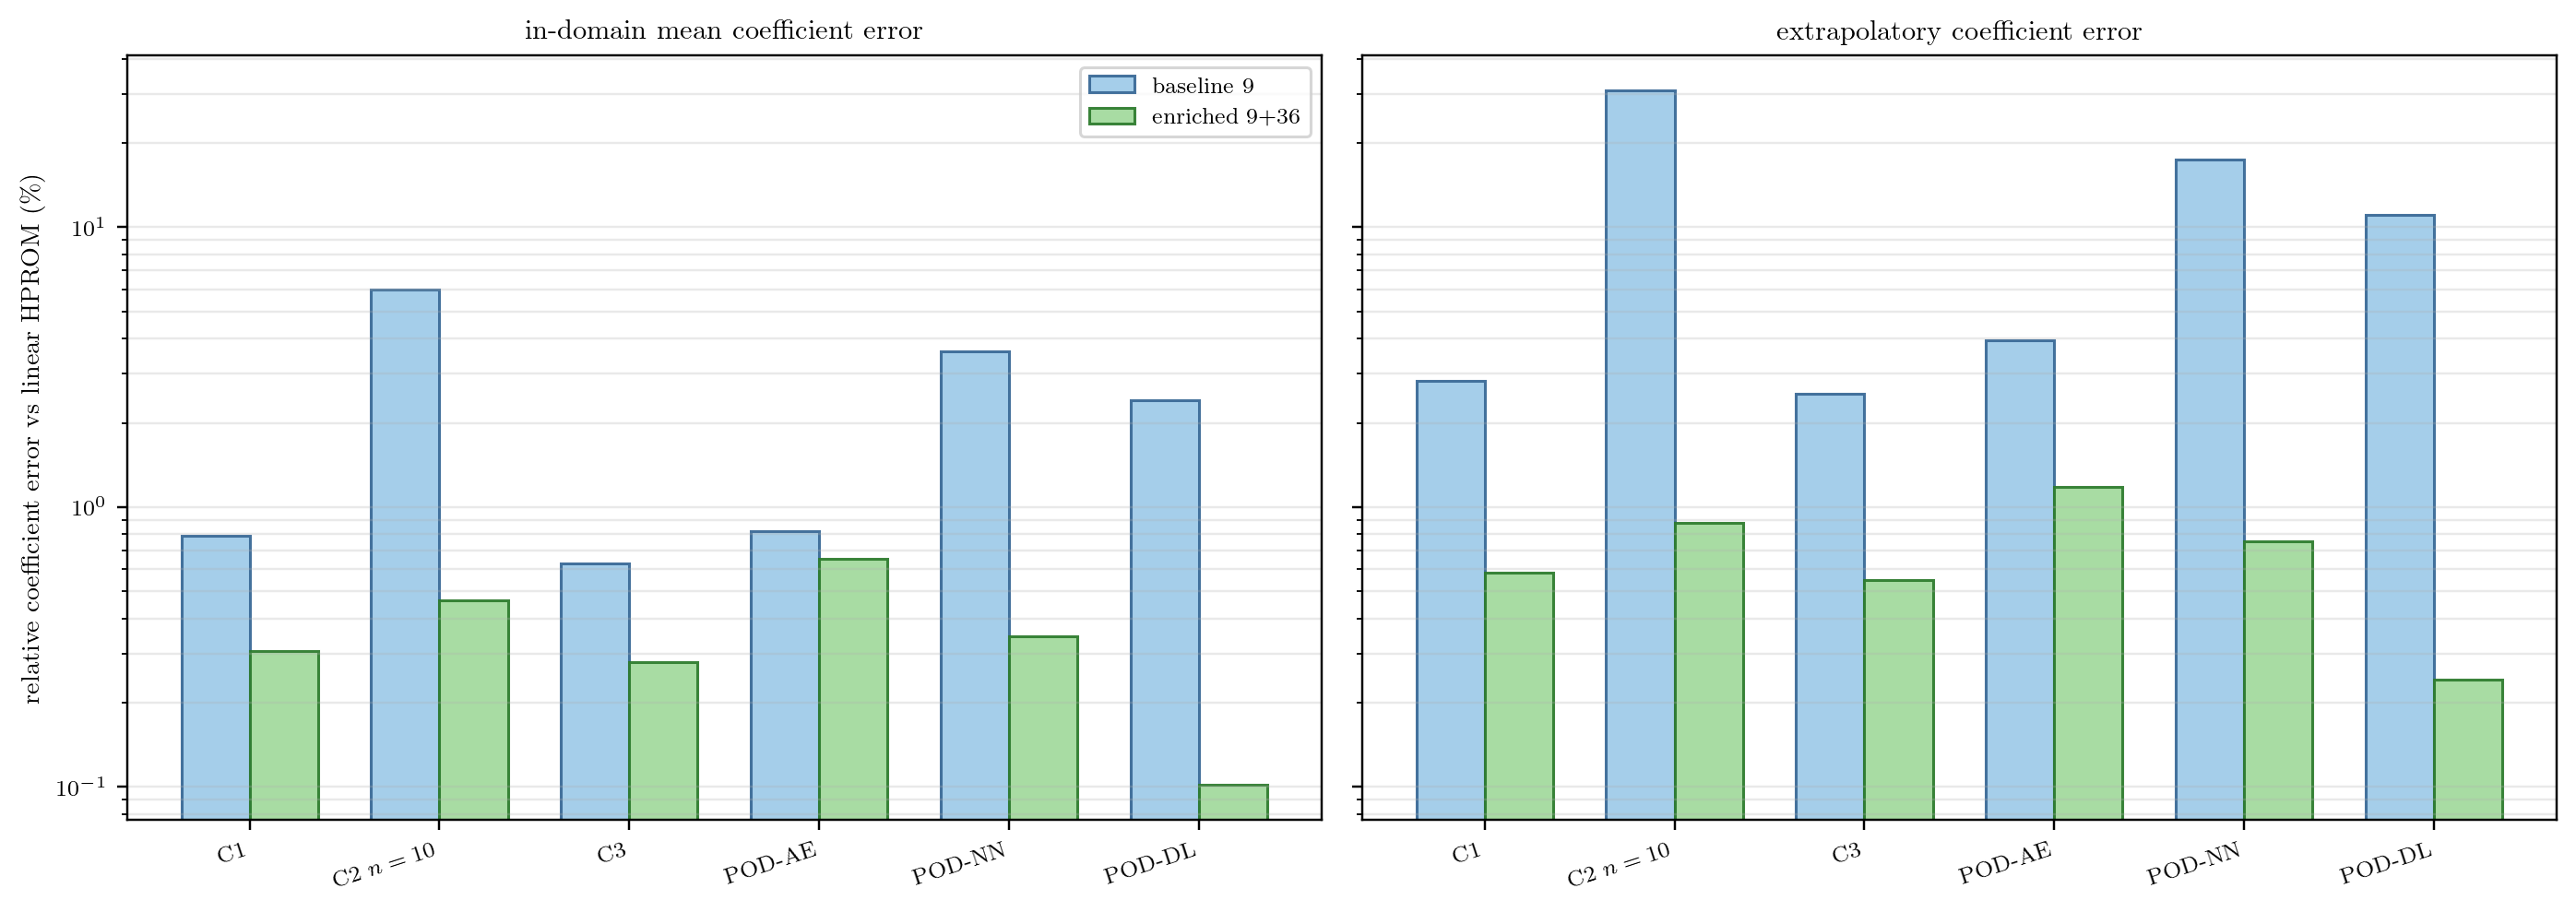
\includegraphics[width=0.98\textwidth]{Figures/hprom_only/hprom_enrichment_coeff_error_comparison.png}
\caption{Effect of HPROM coefficient-data enrichment on global coefficient error.  Enrichment reduces the Case--2
tail error by more than one order of magnitude at the extrapolatory point, while retaining sub-percent global
coefficient errors for the other intrusive closures.}
\label{fig:hprom-enrichment-coeff}
\end{figure}

\begin{figure}[H]
\centering
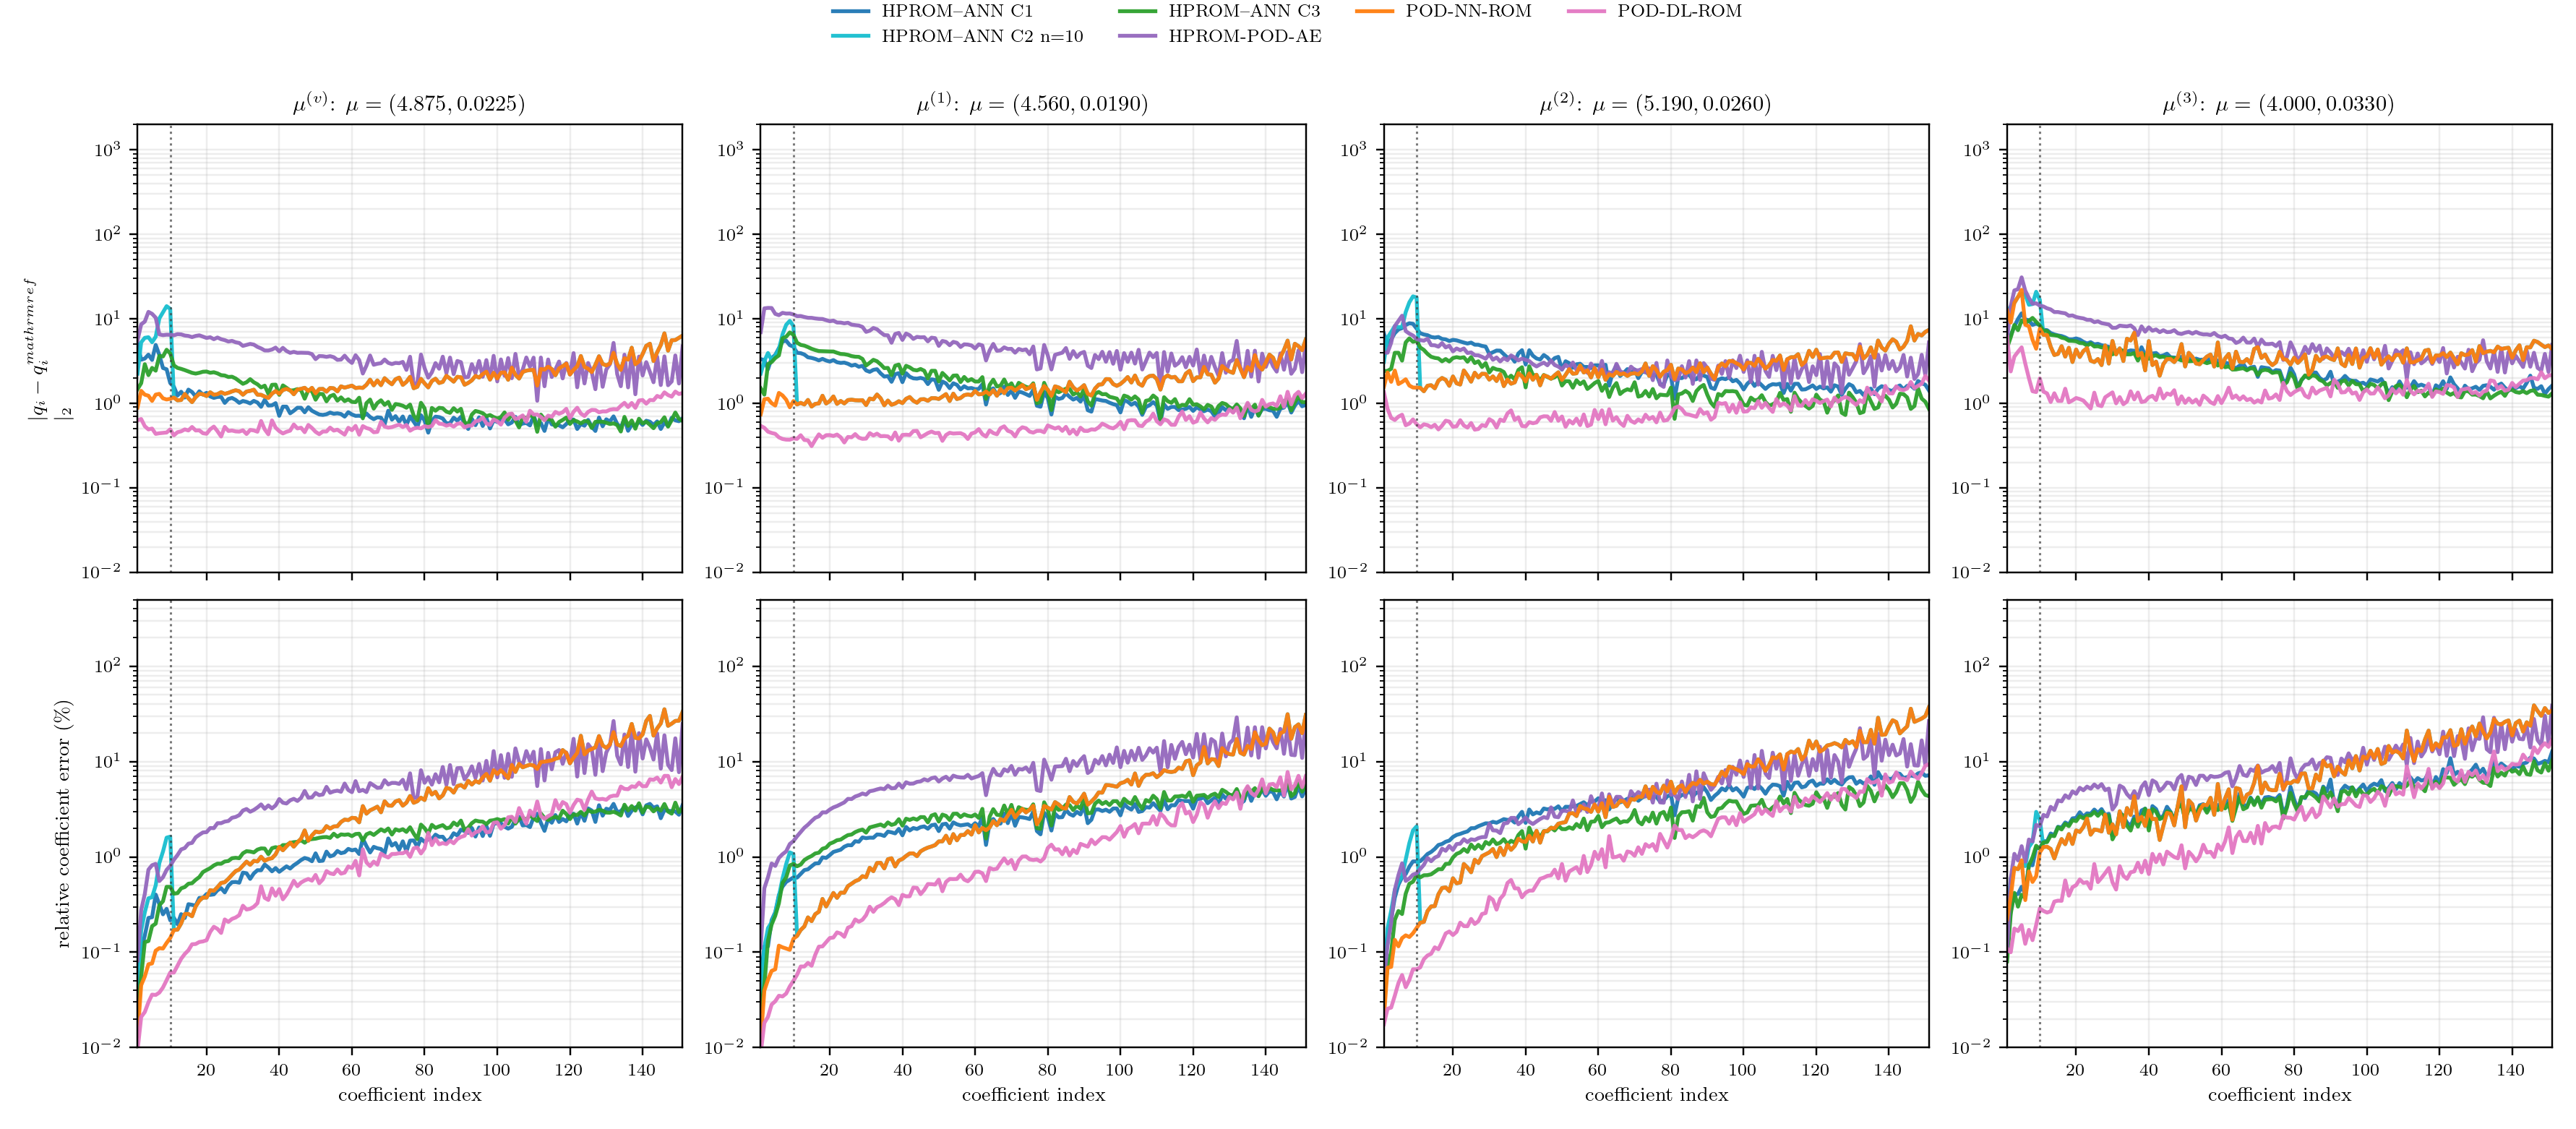
\includegraphics[width=0.98\textwidth]{Figures/hprom_only/hprom_enriched_coeff_abs_rel_errors.png}
\caption{Enriched HPROM online coefficient errors against the enriched linear-HPROM reference.  The plotted set is
identical to Fig.~\ref{fig:hprom-coeff-rel-errors}: Case 1, Case 2 with \(n=10\), Case 3, PROM--POD--AE,
POD--NN--ROM, and POD--DL--ROM.  Shared ordinate ranges permit a direct baseline--enriched comparison.}
\label{fig:hprom-enriched-coeff-errors}
\end{figure}

Coefficient space confirms that this is not merely cancellation in the state norm.  The Case--2 \(n=10\)
in-domain mean coefficient error decreases from \(5.966\%\) to \(0.464\%\), and its extrapolatory coefficient
error decreases from \(30.777\%\) to \(0.876\%\).  The linear HPROM reference is unchanged; the observed
improvement therefore comes from coefficient coverage rather than a different linear basis or a more accurate
linear cubature rule.  The \(n=20\) variant remains in the baseline comparison and the dedicated Case--2 diagnostic;
it is omitted from the paired enrichment figures because the corresponding PROM enrichment campaign uses the
production \(n=10\) split only.

\paragraph{Direct maps trained on linear-HPROM data.}
POD--NN--ROM and POD--DL--ROM do not evaluate a residual and therefore are not HPROM solvers; they have no ECM
approximation error.  Their baseline and enriched values are included in the final two rows of
Tables~\ref{tab:hprom-enrichment-online} and~\ref{tab:hprom-enrichment-coeff}, below a horizontal rule, rather
than being reported in a separate table.  This keeps the direct maps beside the intrusive models trained on the
same coefficient data while preserving the distinction between a sampled-residual HPROM and a pure regression
map.  The HPROM Case~2 closure uses the very same POD--NN master map for its injected secondary block, so its
comparison with the direct map isolates the consequence of residual correction rather than a change of regressor.

The baseline direct maps expose the same coverage limitation as Case 2.  The POD--NN--ROM in-domain mean state
error falls from \(1.607\%\) to \(0.458\%\) after enrichment, and its extrapolatory error falls from \(7.401\%\)
to \(0.926\%\).  The corresponding POD--DL--ROM values fall from \(1.144\%\) to \(0.449\%\) in-domain and from
\(4.753\%\) to \(0.869\%\) at extrapolation.  Thus, the improvement is due entirely to coefficient-data coverage,
not to a sampled residual solve.  Their state and coefficient reductions are reported in the same paired tables and
all-model bar figures as the residual-evaluating methods, ruling out an interpretation based only on cancellation in
the state norm.

\begin{figure}[H]
\centering
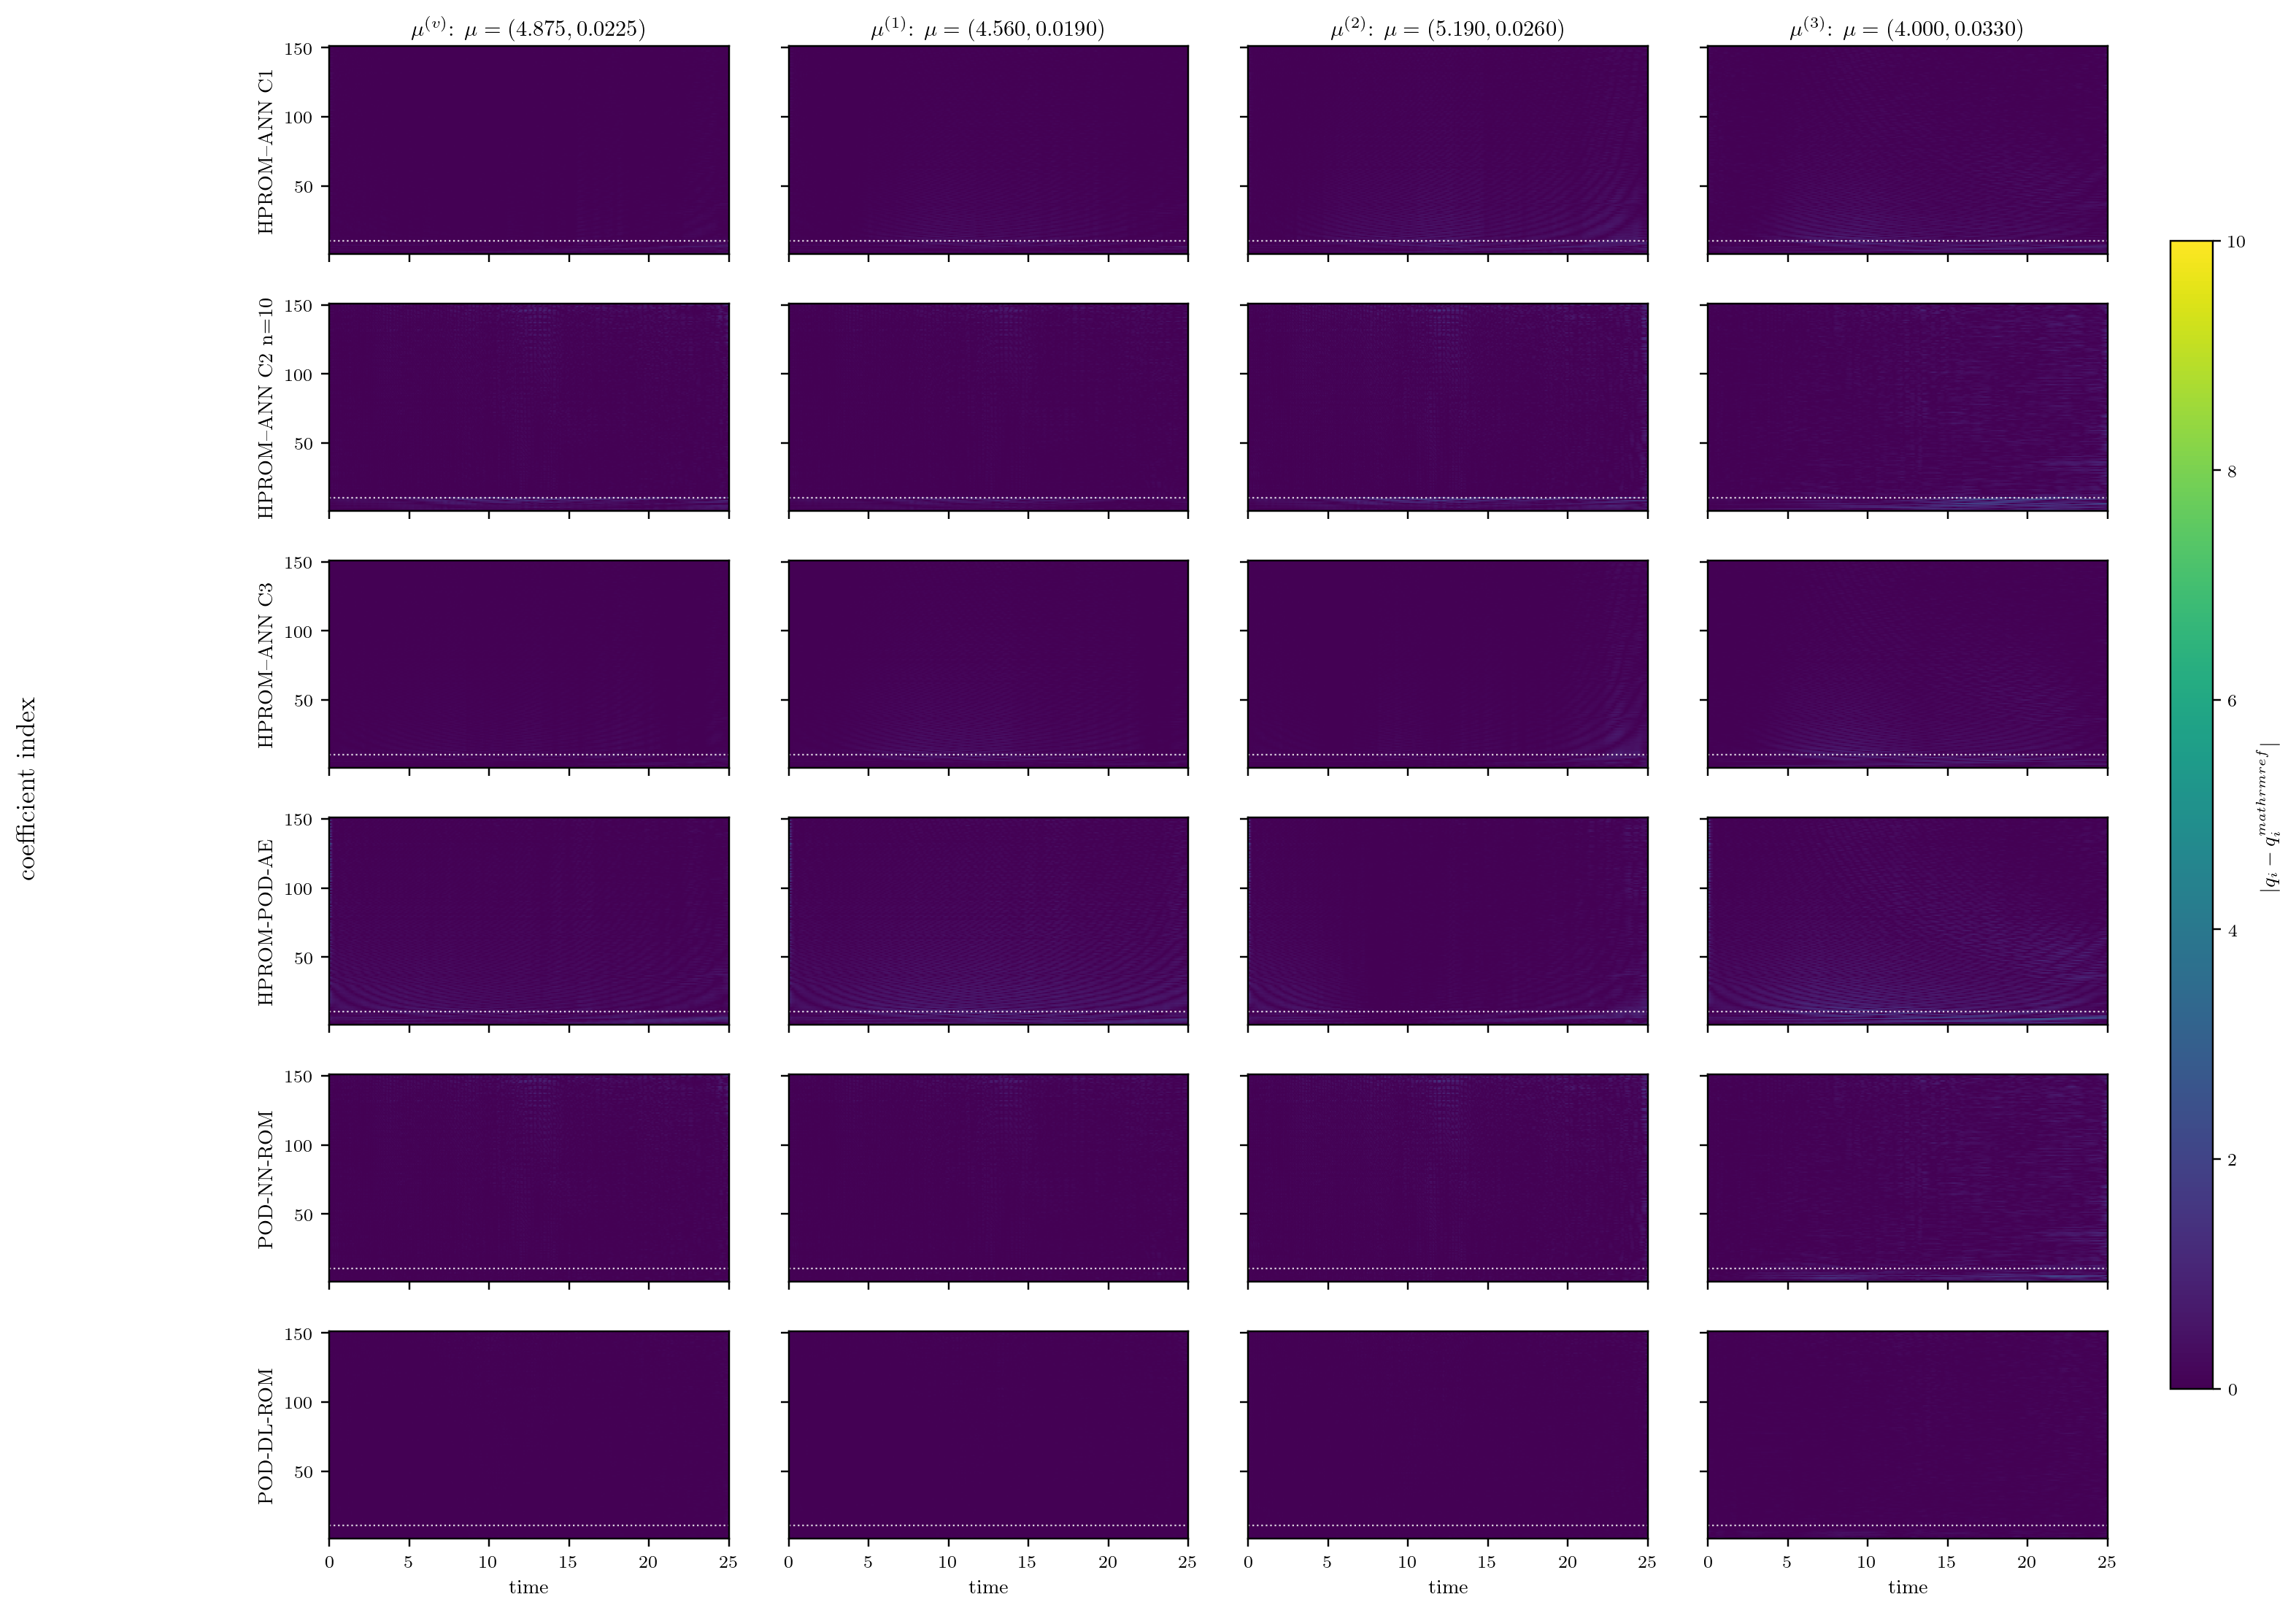
\includegraphics[width=0.98\textwidth]{Figures/hprom_only/hprom_enriched_coeff_abs_heatmaps.png}
\caption{Enriched HPROM time-by-coefficient absolute errors against the enriched linear HPROM.  Rows include the four
intrusive learned HPROMs followed by POD--NN--ROM and POD--DL--ROM.  The colour range and coefficient-10 separator
are identical to the baseline HPROM heatmap in Fig.~\ref{fig:hprom-coeff-abs-heatmaps}.}
\label{fig:hprom-enriched-coeff-abs-heatmaps}
\end{figure}

\begin{figure}[H]
\centering
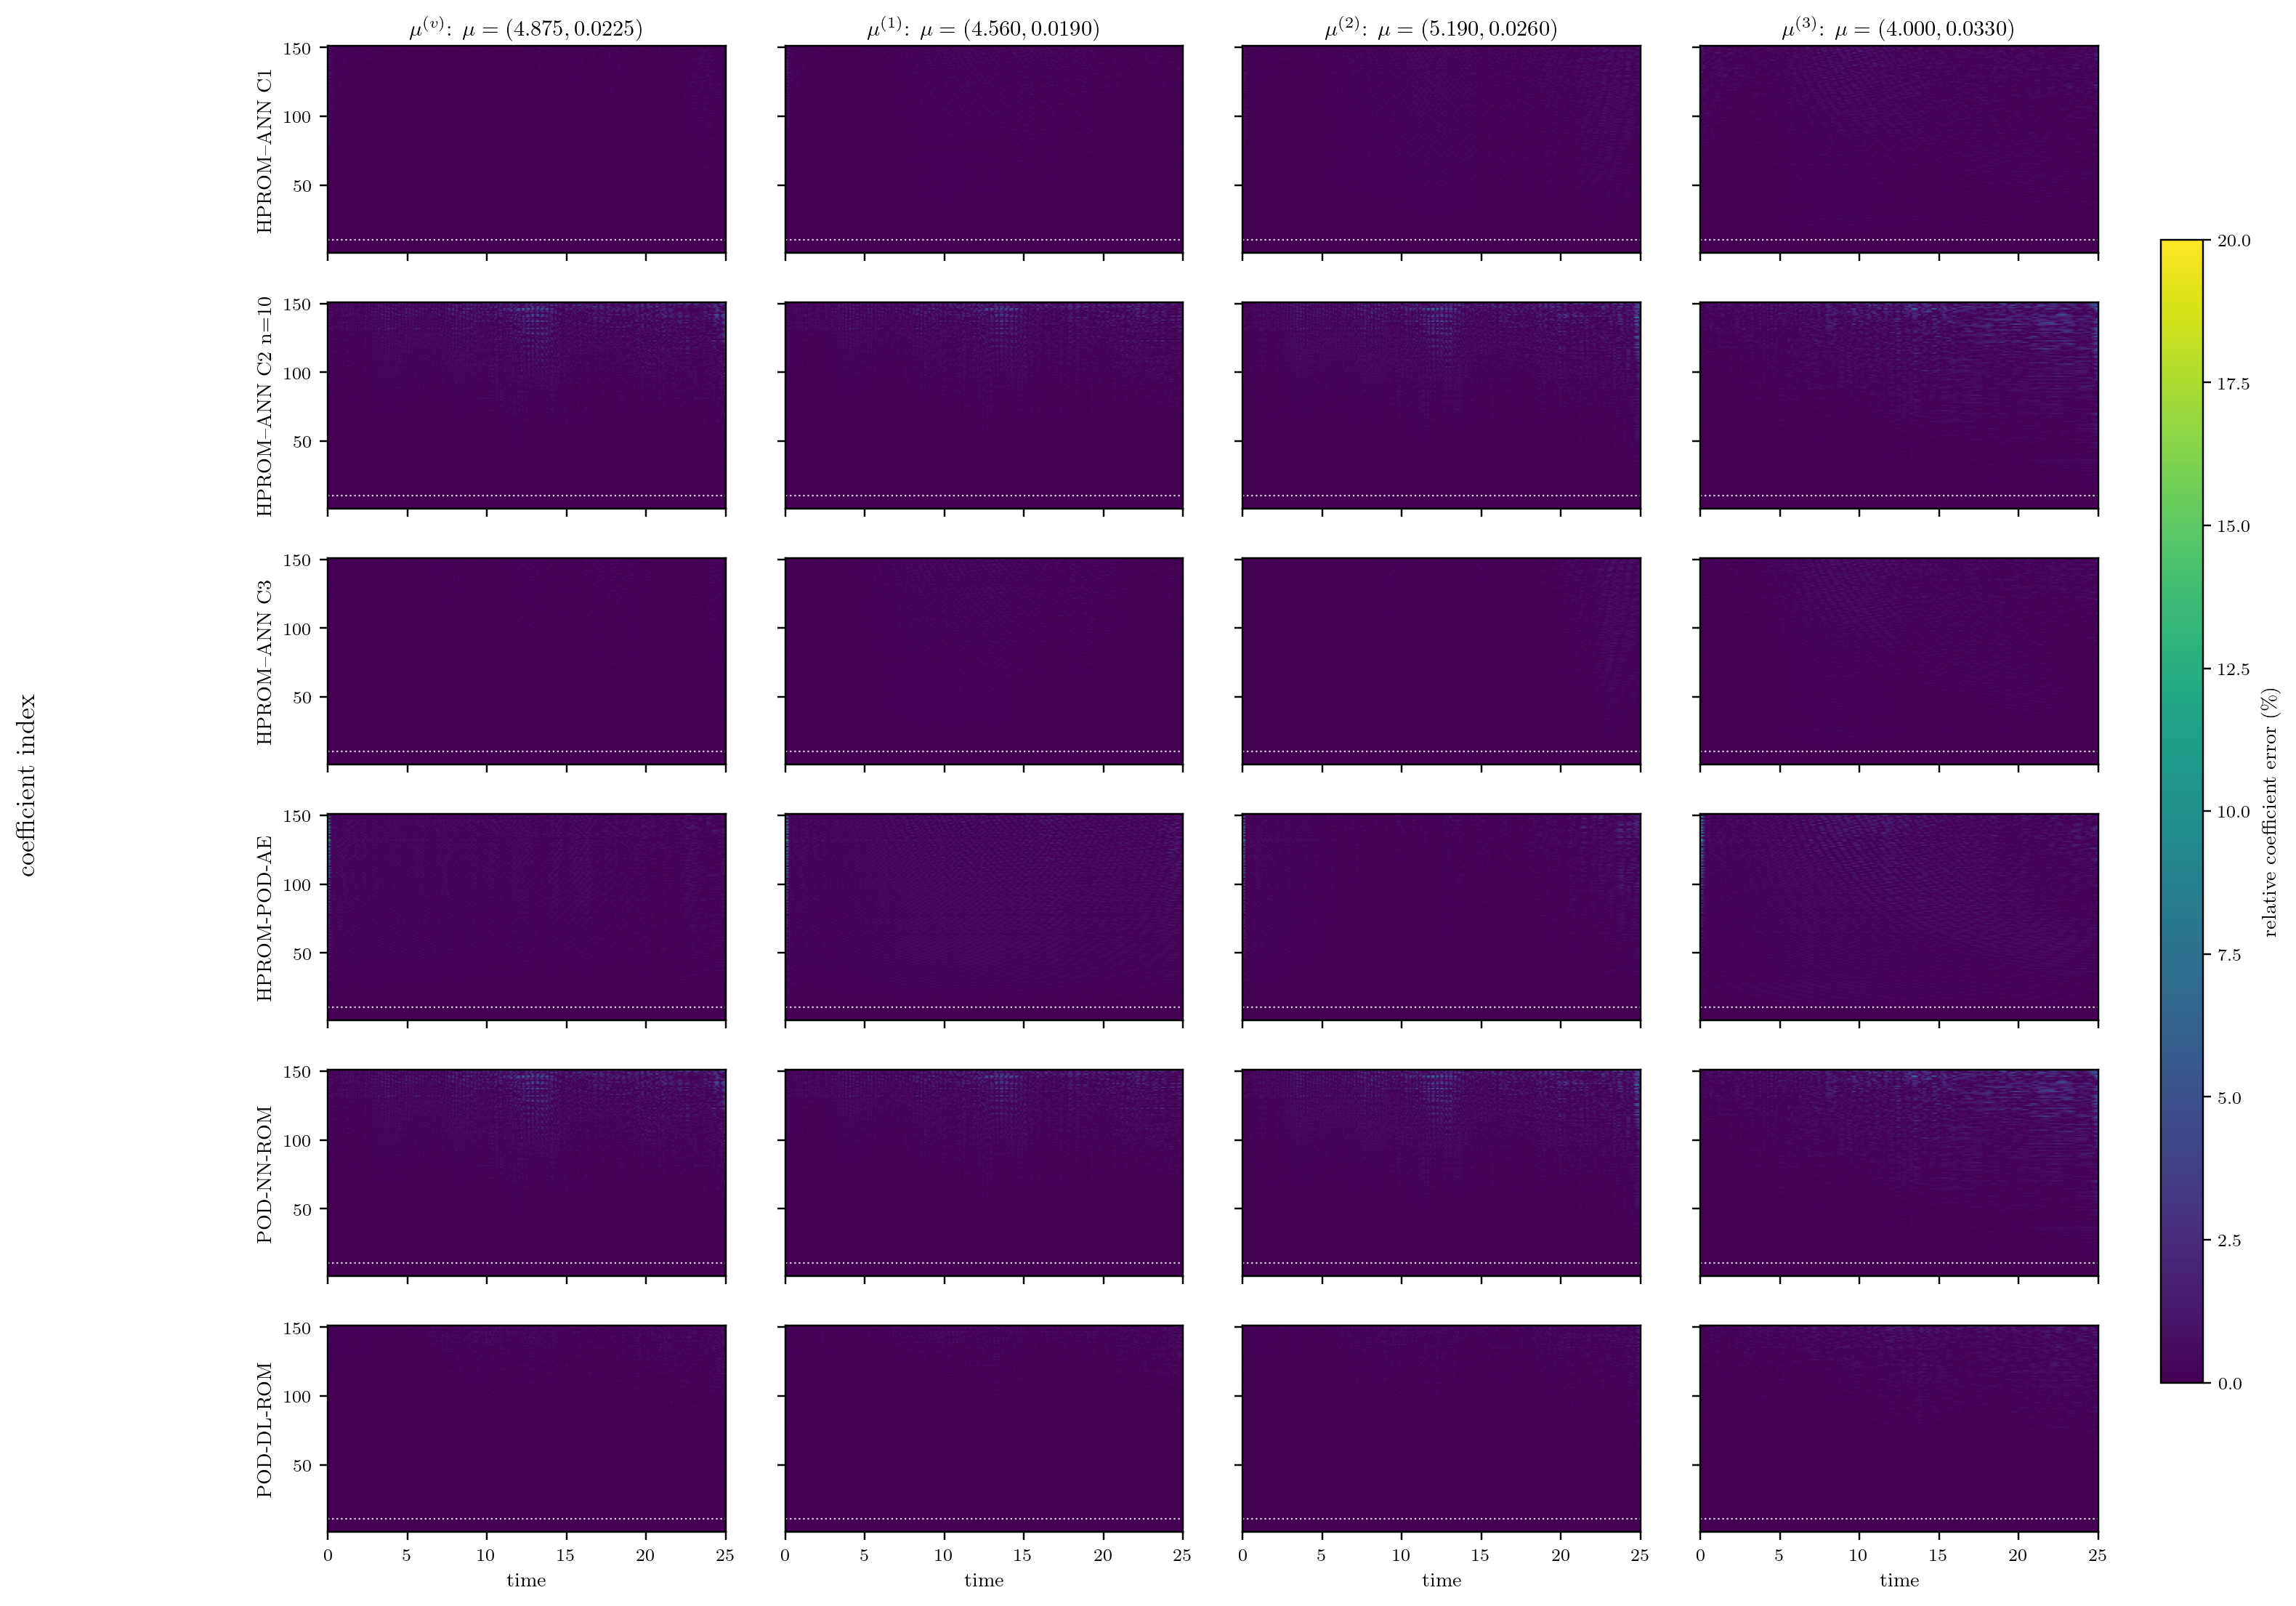
\includegraphics[width=0.98\textwidth]{Figures/hprom_only/hprom_enriched_coeff_rel_heatmaps.png}
\caption{Enriched HPROM time-by-coefficient relative errors.  The shared \(0\)--\(20\%\) colour range exposes the
low-error structure recovered by enrichment while clipping only larger values.}
\label{fig:hprom-enriched-coeff-rel-heatmaps}
\end{figure}

\begin{figure}[H]
\centering
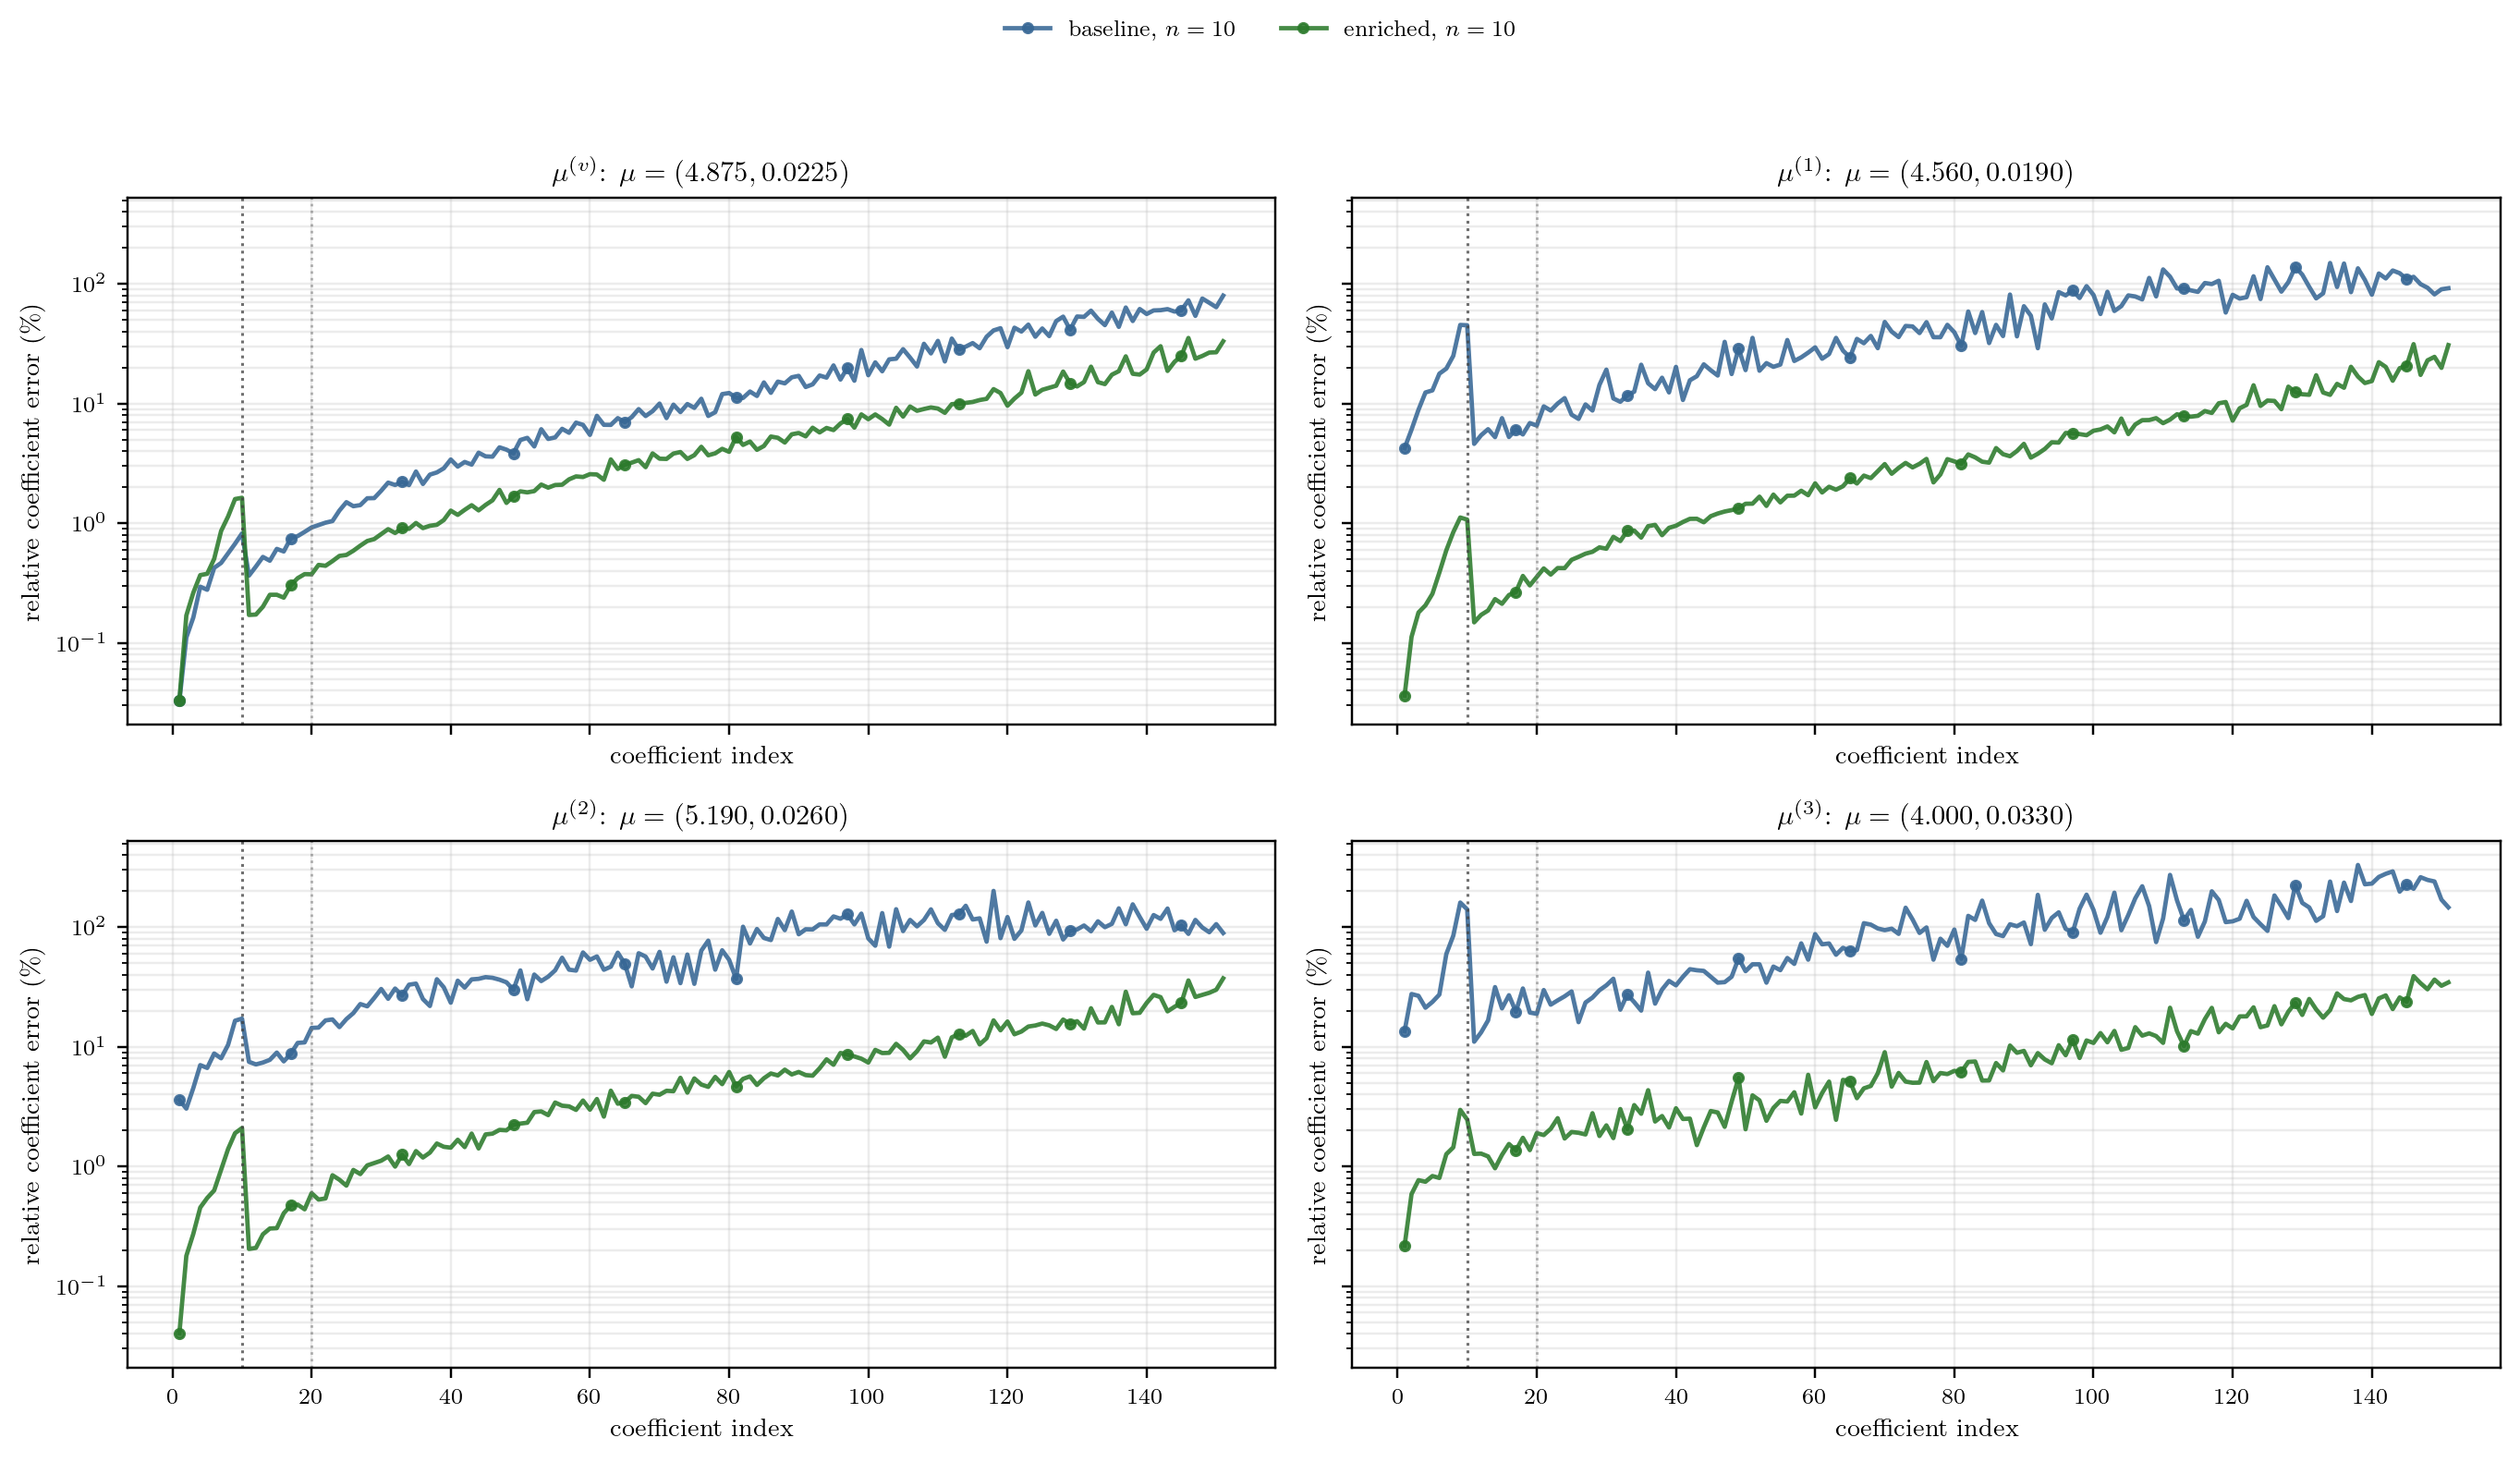
\includegraphics[width=0.98\textwidth]{Figures/hprom_only/hprom_enrichment_case2_coeff_rel_errors.png}
\caption{Case--2 per-coefficient HPROM relative error before and after coefficient-data enrichment for \(n=10\).
The dotted vertical line marks the separation between the ten residual-solved primary coordinates and the
ANN-injected secondary tail.  The linear HPROM coefficient trajectory is the reference.}
\label{fig:hprom-enrichment-case2-coeff}
\end{figure}

Figure~\ref{fig:hprom-enrichment-case2-coeff} gives the mechanism behind the aggregate results.  In the baseline,
the injected tail is inaccurate at most secondary coordinates, especially away from the training grid.  Enrichment
substantially lowers those tail errors.  The sampled residual solve then needs only to correct the leading
coordinates, which is why even Case 2 with \(n=10\) returns to the linear-HPROM state-accuracy scale.

\section{Conclusions}
The PROM and HPROM studies support the following conclusions.
\begin{enumerate}
  \item The fixed MLSPG-sensitive linear PROM provides a reproducible coefficient teacher and state-accuracy
  reference for this benchmark.
  \item With only nine training trajectories, direct parameter--time prediction of all 151 coefficients is the
  limiting task.  This affects both the POD--NN--ROM and the Case 2 injected tail.
  \item Solving more primary coordinates in Case 2 can help, but the matched-rule HPROM sweep is non-monotone at
  small $n$ and does not reach the linear-HPROM reference by $n=50$.  With a fixed $n=10$ rule, imposed tail
  error changes the primary coordinates recovered by the residual solve; tail accuracy is therefore essential.
  \item PROM data enrichment changes the picture substantially.  Keeping the architecture and basis fixed, the
  9+36 PROM trajectory set reduces validation and online coefficient errors and brings the learned state errors close
  to the linear PROM level.
  \item The baseline HPROM with 2\% parameter--time stratified snapshots preserves the main PROM conclusion for
  Case 1, Case 3, and PROM--POD--AE: these learned intrusive models remain close to the linear HPROM reference at
  in-domain points.
  \item Case 2 is the residual-sampling stress test.  With nine coefficient trajectories, \(n=10\) is highly
  sensitive to the injected secondary tail.  The fixed-rule diagnostic demonstrates that this sensitivity is
  residual feedback, not solely reconstruction error, while the matched-rule sweep shows improvement only once
  a sufficiently large primary block is solved.
  \item HPROM coefficient-data enrichment transfers the PROM-level gain without changing the linear HPROM reference
  or adding HDM training snapshots.  The \(9+36\) campaign reduces Case--2 \(n=10\) from \(2.641\%\) to \(0.468\%\)
  in-domain and from \(13.098\%\) to \(0.921\%\) at extrapolation, placing it on the same practical accuracy scale as
  the linear HPROM.
  \item The same enrichment effect is present without an online residual solve.  Both direct maps improve sharply,
  particularly at extrapolation, confirming that coefficient-data coverage is a primary limitation.  These maps do
  not quantify ECM error, however, so they complement rather than replace the intrusive HPROM comparisons.
\end{enumerate}


% Appendix retained from the original metric study.

\appendix

\section{Matched Case--2 PROM--HPROM Diagnostics}
\label{app:case2-prom-hprom-diagnostics}

The main results deliberately separate the full-residual PROM from the
ECM-hyperreduced HPROM.  This appendix makes that separation explicit for the
Case--2 parameter--time closure with \(n=10\) solved primary coordinates.  The
comparison is diagnostic rather than a claim that hyperreduction produces a
single uniform error penalty.  Both state errors are measured against the same
HDM trajectory.  In contrast, each coefficient error is measured against the
full linear reference associated with the corresponding solver: the linear
PROM for the solid curves and the linear HPROM for the dashed curves.  This is
the consistent reference for the prescribed-tail experiment, whose
perturbation is itself defined relative to the respective linear tail.

Figure~\ref{fig:app-case2-prom-hprom-tail} compares the response to the same
imposed secondary-coordinate discrepancy.  The actual master-map tail levels
are marked separately because they are not the same for PROM and HPROM.  At
the verification parameter, the zero-tail states are close, but the HPROM is
substantially more sensitive once the comparison is made at a common
disturbance level.  For example, at a \(50\%\) imposed tail error, the state
error is \(12.35\%\) for HPROM versus \(5.31\%\) for PROM, while the error in
the ten solved coordinates is \(27.87\%\) versus \(7.82\%\), respectively.
The same qualitative amplification is visible at the two off-grid points and
at extrapolation.  Thus, this experiment isolates an additional
residual-sampling sensitivity of the fixed ECM rule; it does not attribute the
entire Case--2 error to the neural map.

\begin{figure}[H]
\centering
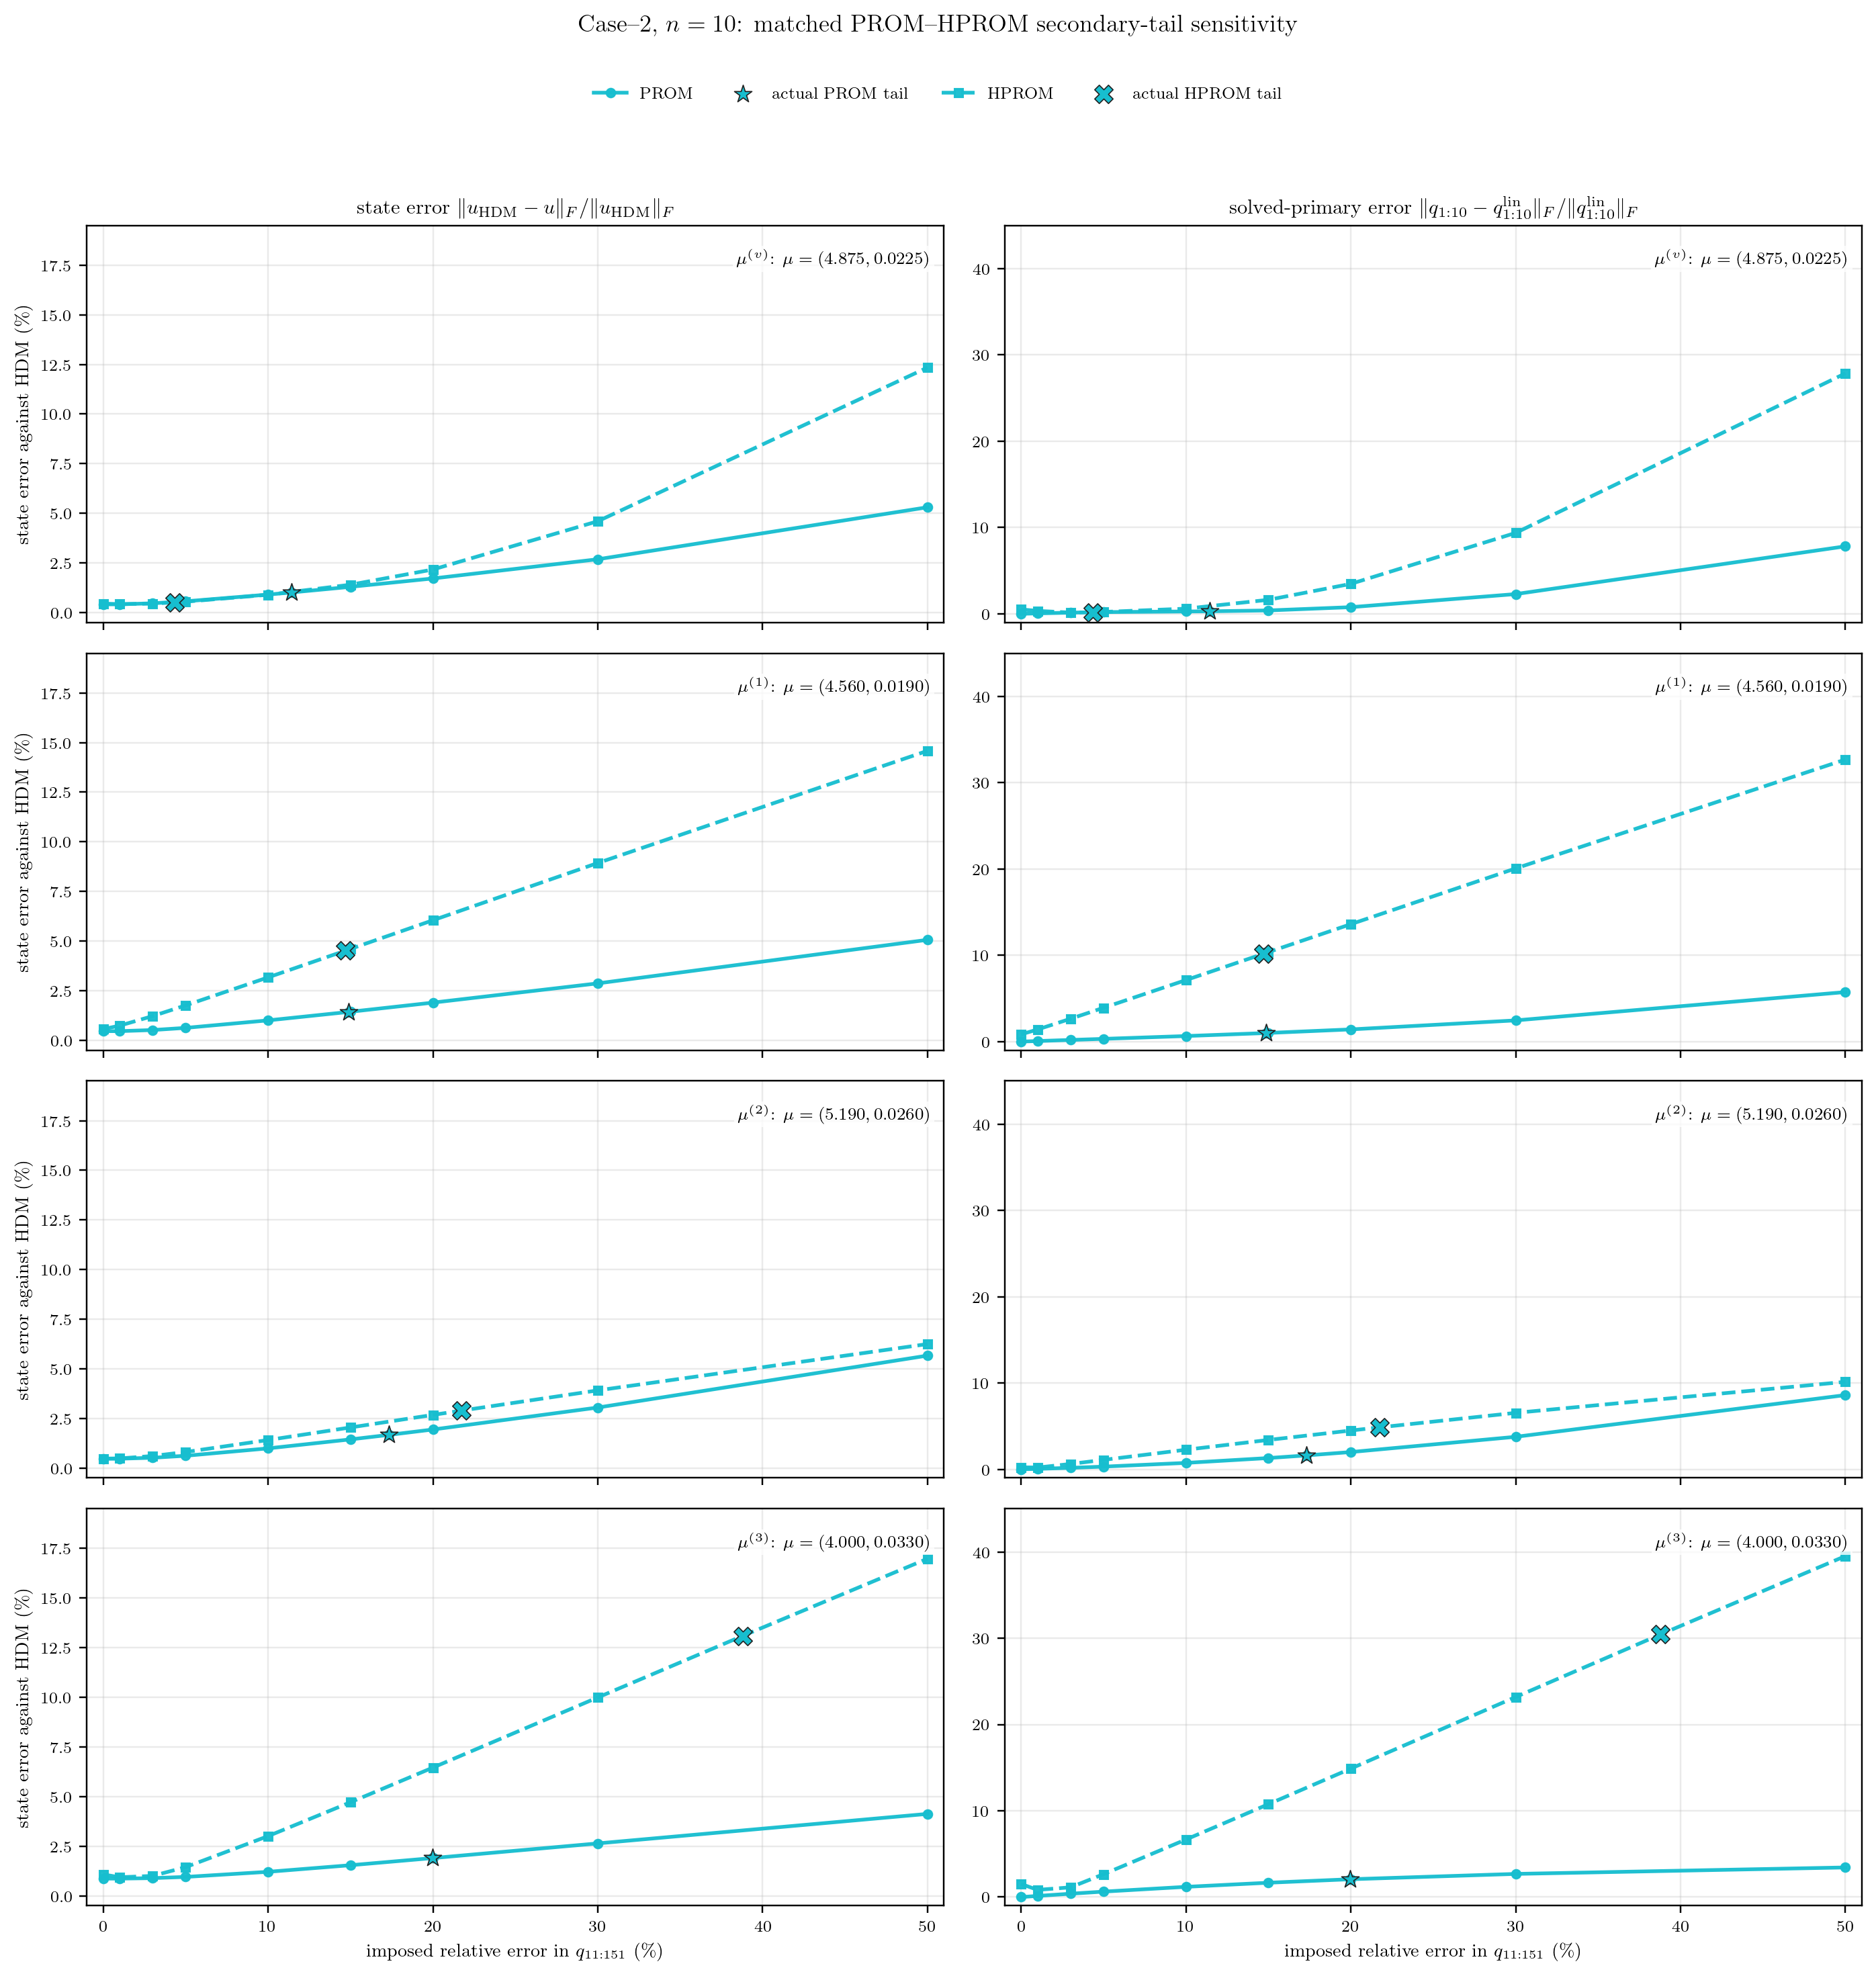
\includegraphics[width=\textwidth]{Figures/appendix/prom_hprom_case2_n10_tail_sensitivity.png}
\caption{Matched Case--2 secondary-tail diagnostic with \(n=10\).  Rows are,
from top to bottom, the verification point, the two off-grid points, and the
extrapolatory point.  Solid curves are the full-residual PROM and dashed
curves are the ECM-HPROM.  Both use the same trained parameter--time map; the
star and cross mark the actual PROM and HPROM master-map tail errors,
respectively.  State error is measured against the HDM in both cases.  Each
primary-coordinate error is measured against the method-matched full linear
reference trajectory.}
\label{fig:app-case2-prom-hprom-tail}
\end{figure}

Figure~\ref{fig:app-case2-prom-hprom-nsweep} gives the requested
coefficient-resolved comparison of the two matched-rule sweeps.  Each colour
identifies the same solved dimension \(n\), with PROM shown by a solid line and
HPROM by a dashed line.  Only the common values
\(n\in\{0,3,5,10,20,30,50\}\) are shown because the HPROM diagnostic was run
only through \(n=50\); the \(n=151\) linear references are zero-error
endpoints and are omitted.  The verification panel does not by itself support
a generic HPROM-failure claim.  The systematic discrepancy instead appears
at the off-grid and extrapolatory points, especially in the injected-tail
range \(i>10\), where the dashed HPROM curves remain well above the solid PROM
curves for the same \(n\).  This is the coefficient-level counterpart of the
fixed-tail sensitivity observed in Figure~\ref{fig:app-case2-prom-hprom-tail}.

\begin{figure}[H]
\centering
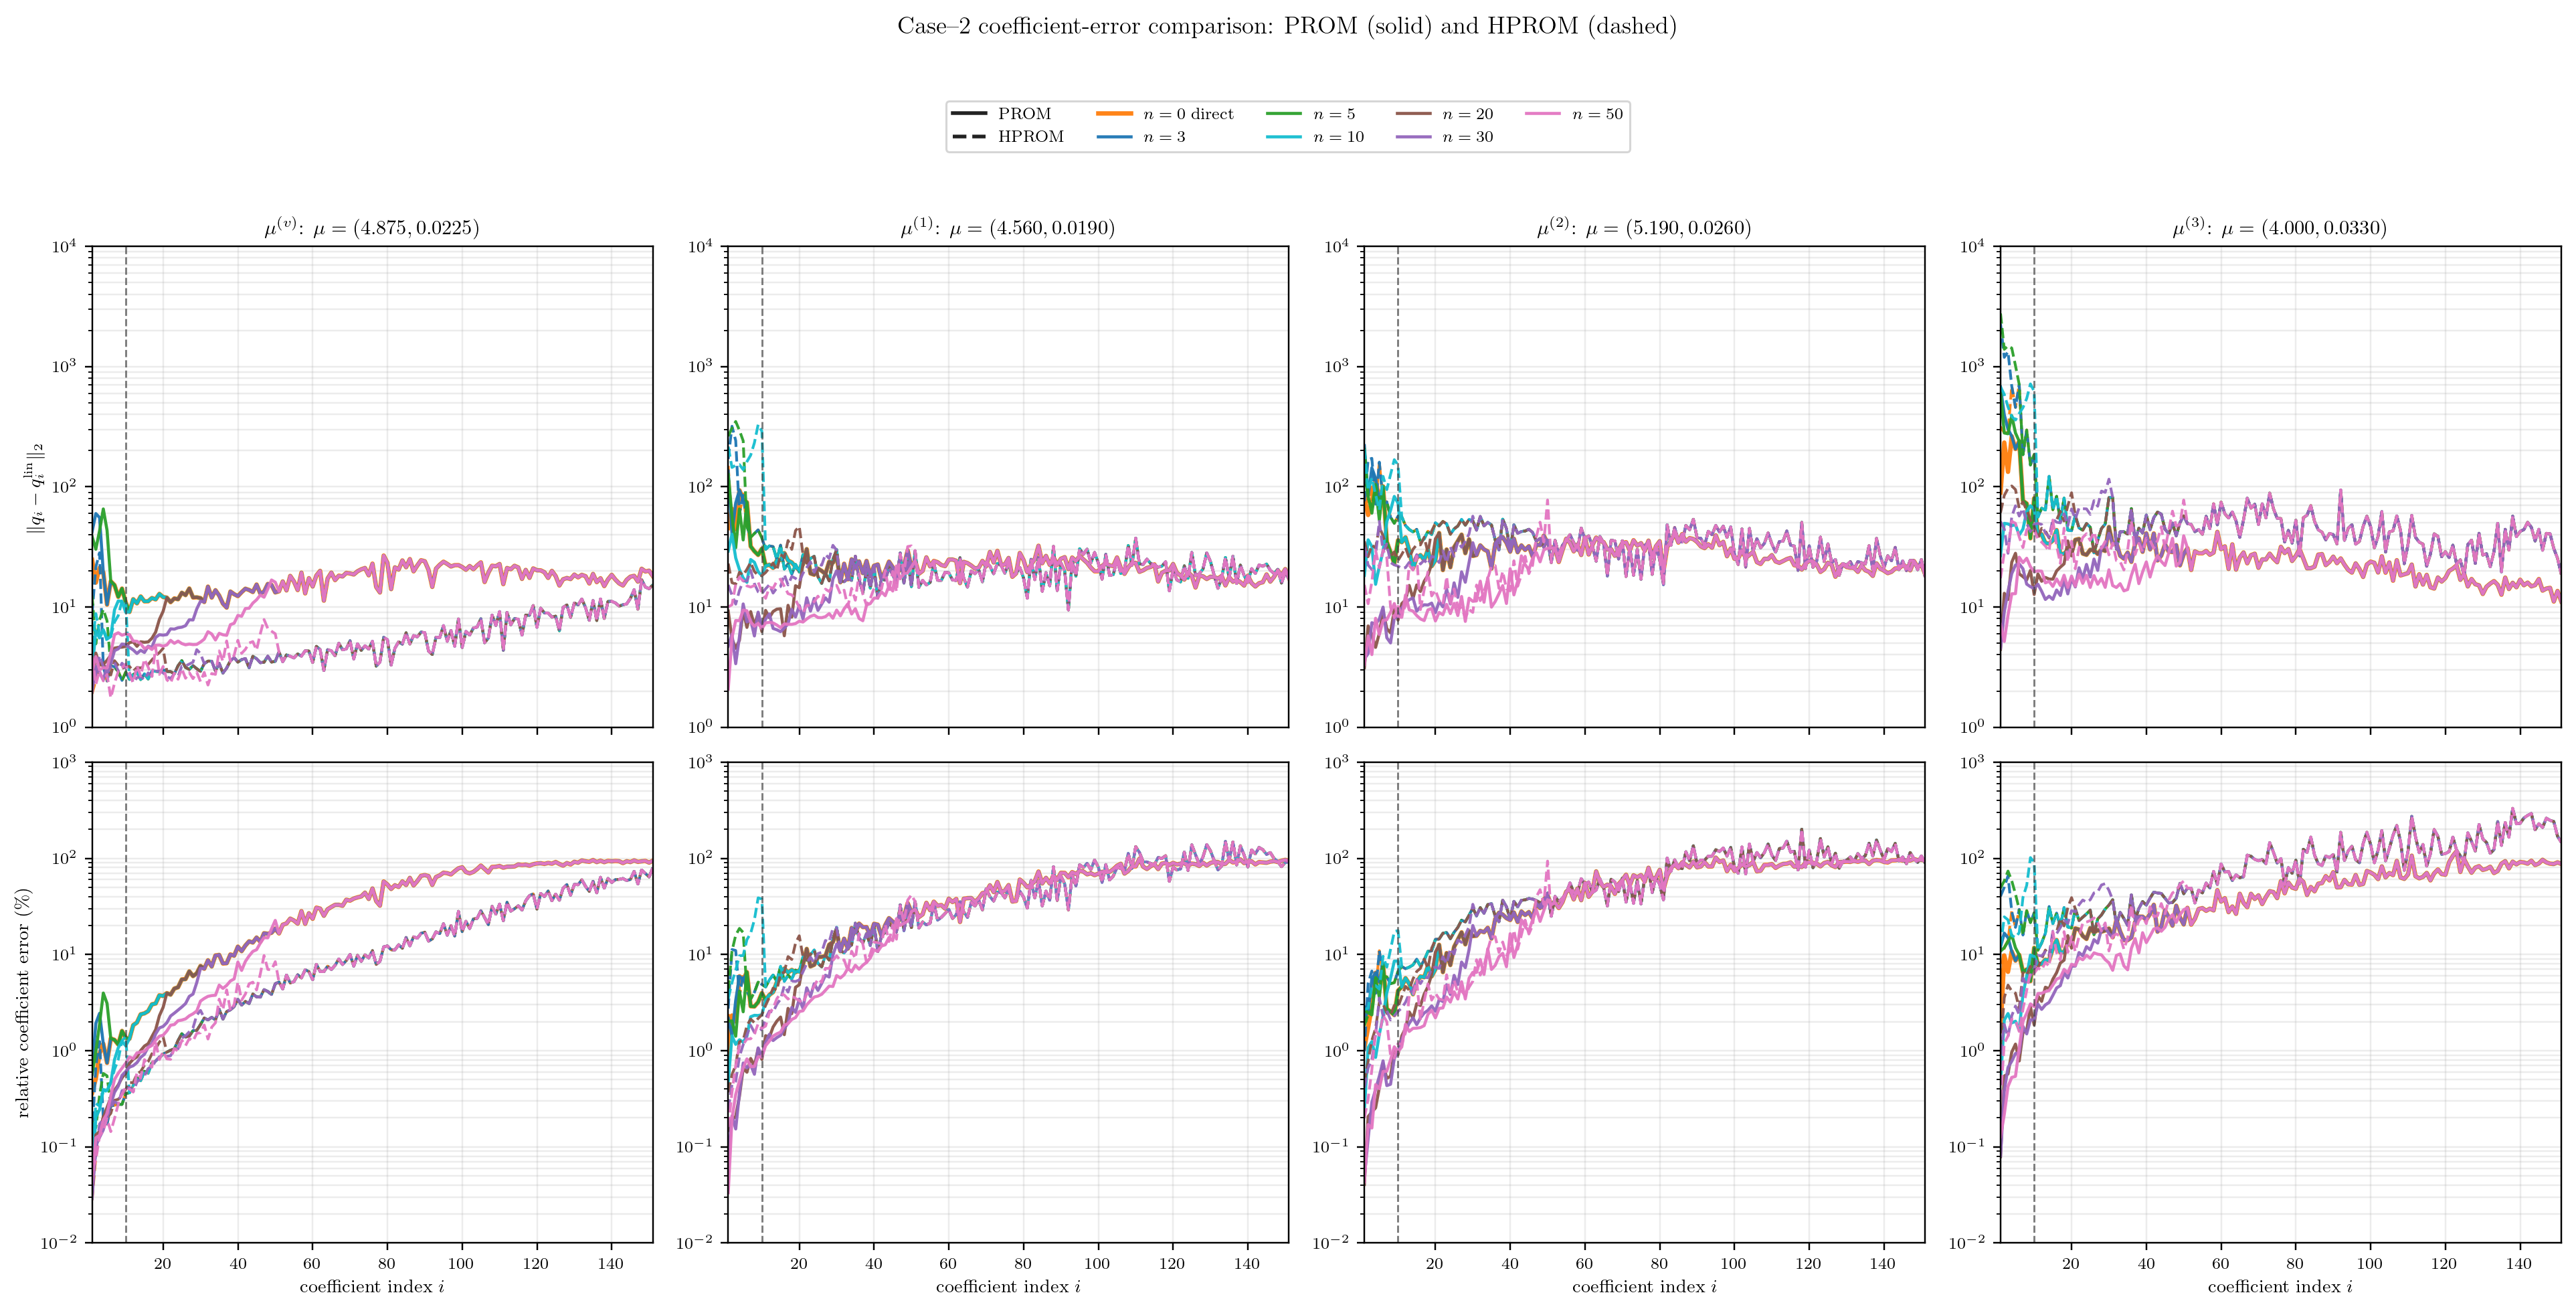
\includegraphics[width=\textwidth]{Figures/appendix/prom_hprom_case2_n_sweep_coefficients_comparison.png}
\caption{Matched Case--2 coefficient-error sweeps.  Columns are ordered as
\(\mu^{(v)}\), \(\mu^{(1)}\), \(\mu^{(2)}\), and \(\mu^{(3)}\).  Top: absolute
time-trajectory coefficient error.  Bottom: relative coefficient error.
Each colour identifies the solved primary dimension \(n\); solid curves are
PROM and dashed curves are HPROM.  The vertical line marks coefficient 10.
Each solver is compared with its own full linear reference trajectory, so the
figure exposes the effect of hyperreduction on the matched Case--2
coefficient sweep without conflating the two distinct linear references.}
\label{fig:app-case2-prom-hprom-nsweep}
\end{figure}

\section{Burgers Basis-Selection Diagnostics}
\label{app:basis-selection-diagnostics}

The $M$-regularized LSPG-sensitive basis was selected through two diagnostics.
The first diagnostic is the low/high transfer operator
$\mathbf T_{LH}$ introduced in \eqref{eq:low-high-transfer}.  Table
\ref{tab:low-high-transfer-summary} reports the singular-value statistics of
this operator over the three Burgers evaluation trajectories.  The
LSPG-sensitive basis reduces the mean value of
$\sigma_{\max}(\mathbf T_{LH})$ by approximately one half relative to the
Euclidean POD basis, and also reduces the 95th percentile and maximum values.
This supports the use of the modified metric as a robustness device for
intrusive nonlinear reduced models: if the nonlinear closure, decoder, or
surrogate produces errors in the unresolved part of the representation, the
resulting feedback into the resolved coordinates through the LSPG normal
equations is less amplifying.

\begin{table}[H]
\centering
\caption{Burgers low/high transfer diagnostic for basis selection. The table reports statistics of $\sigma_{\max}(\mathbf T_{LH})$ and of the corresponding $M$-weighted state gain $g_M$ over the original three evaluation trajectories.}
\label{tab:low-high-transfer-summary}
\resizebox{\textwidth}{!}{%
\begin{tabular}{lrrrrrr}
\toprule
Basis & $\operatorname{mean}\sigma_{\max}(T_{LH})$ & $\operatorname{p95}\sigma_{\max}(T_{LH})$ & $\max\sigma_{\max}(T_{LH})$ & $\operatorname{mean}g_M$ & $\operatorname{p95}g_M$ & $\max g_M$ \\
\midrule
Euclidean POD & 3.078e-02 & 3.668e-02 & 4.088e-02 & 3.078e-02 & 3.668e-02 & 4.088e-02 \\
LSPG-sensitive POD & 1.548e-02 & 2.244e-02 & 2.433e-02 & 1.599e-02 & 2.339e-02 & 2.559e-02 \\
\bottomrule
\end{tabular}

}
\end{table}

As a complementary check, we perturb only the high-coordinate block of an
oracle reconstruction and measure the induced deviation from the linear
reduced trajectory.  This test is implemented with the Case~2 partition because
it isolates the most direct contamination mechanism: the high block is injected
independently of the online low-coordinate solve.  Table
\ref{tab:metric-oracle-diagnostic} reports averages over the original
verification point, two off-grid points, and five random seeds for the
perturbed cases.
The $M$-regularized LSPG-sensitive basis slightly increases the unperturbed
linear error in this preliminary test, but reduces the high-to-low
contamination measured against the linear reference, especially in the
resolved coordinates.  The intended role of the metric is broader than this
specific test: it provides a protective basis choice for nonlinear intrusive
models in which learned high coordinates or decoded manifold corrections may
contain approximation error.  This diagnostic is not used as a standalone
performance result; it supports the basis choice used in the main Burgers
campaign.

\begin{table}[H]
\centering
\caption{Oracle high-mode perturbation diagnostic for basis selection. Errors are averaged over $\bm\mu^{(v)}$, $\bm\mu^{(1)}$, $\bm\mu^{(2)}$; perturbed rows also average over five random seeds.}
\label{tab:metric-oracle-diagnostic}
\resizebox{\textwidth}{!}{
\begin{tabular}{lccccc}
\toprule
Basis metric &
Unperturbed $\varepsilon_u$ vs HDM (\%) &
$1\%$ pert., $\varepsilon_u$ vs linear (\%) &
$1\%$ pert., $\varepsilon_q^{\mathrm{low}}$ vs linear (\%) &
$2\%$ pert., $\varepsilon_u$ vs linear (\%) &
$2\%$ pert., $\varepsilon_q^{\mathrm{low}}$ vs linear (\%) \\
\midrule
Euclidean POD & 0.441 & 0.091 & 0.014 & 0.183 & 0.045 \\
$M$-regularized LSPG-sensitive POD & 0.448 & 0.088 & 0.012 & 0.177 & 0.035 \\
\bottomrule
\end{tabular}
}
\end{table}

\bibliographystyle{unsrt}
\bibliography{bibliography}

\end{document}
